\documentclass[12pt,UTF8]{ctexart}
\usepackage{titling,setspace,caption}
\usepackage{enumerate,enumitem}
\usepackage{amsmath,amssymb,amsfonts}
\usepackage{listings}
\usepackage{comment}
\usepackage{float}
\usepackage{graphicx}
\usepackage{multicol,multirow,bigstrut}
\usepackage{fancyhdr} % 页眉
\usepackage{rotating}
\usepackage{ctex,titlesec}
\usepackage[export]{adjustbox} % 图片左对齐
\usepackage[unicode=true,%本行非常重要 支持中文目录hyperref CJKbookmarks对二级目录没用
	colorlinks,
	linkcolor=black,
	anchorcolor=black,
	citecolor=black,
	CJKbookmarks=false]{hyperref}
\usepackage{xcolor}
\usepackage{geometry}
\geometry{top=25.4mm,bottom=25.4mm,left=31.8mm,right=31.8mm}
\pagestyle{plain}%删除页眉
\CTEXsetup[format={\large\bfseries}]{section}
\renewcommand\maketitlehooka{\null\mbox{}\vfill} % 标题页
\renewcommand\maketitlehookd{\vfill\null}

\newcommand{\chuhao}{\fontsize{42.2pt}{\baselineskip}\selectfont}
\newcommand{\xiaochu}{\fontsize{36.1pt}{\baselineskip}\selectfont}
\newcommand{\yihao}{\fontsize{26.1pt}{\baselineskip}\selectfont}
\newcommand{\xiaoyi}{\fontsize{24.1pt}{\baselineskip}\selectfont}
\newcommand{\erhao}{\fontsize{22.1pt}{\baselineskip}\selectfont}
\newcommand{\xiaoer}{\fontsize{18.1pt}{\baselineskip}\selectfont}
\newcommand{\sanhao}{\fontsize{16.1pt}{\baselineskip}\selectfont}
\newcommand{\xiaosan}{\fontsize{15.1pt}{\baselineskip}\selectfont}
\newcommand{\sihao}{\fontsize{14.1pt}{\baselineskip}\selectfont}
\newcommand{\xiaosi}{\fontsize{12.1pt}{\baselineskip}\selectfont}
\newcommand{\wuhao}{\fontsize{10.5pt}{\baselineskip}\selectfont}
\newcommand{\xiaowu}{\fontsize{9.0pt}{\baselineskip}\selectfont}
\newcommand{\liuhao}{\fontsize{7.5pt}{\baselineskip}\selectfont}
\newcommand{\xiaoliu}{\fontsize{6.5pt}{\baselineskip}\selectfont}
\newcommand{\qihao}{\fontsize{5.5pt}{\baselineskip}\selectfont}
\newcommand{\bahao}{\fontsize{5.0pt}{\baselineskip}\selectfont}
\titleformat{\section}{\xiaosi\bfseries}{\chinese{section}、 }{0em}{}
\titleformat{\subsection}{\wuhao\bfseries}{\Roman{subsection}. }{0em}{} %\arabic
\titleformat{\subsubsection}{\wuhao\bfseries}{\roman{subsubsection}. }{0em}{}
% \titlespacing*{hcommandi}{hlefti}{hbefore-sepi}{hafter-sepi}[hright-sepi]
\titlespacing*{\section}{0pt}{0pt}{3pt}
\titlespacing*{\subsection}{0pt}{0pt}{0pt}
\titlespacing*{\subsubsection}{0pt}{0pt}{0pt}
\captionsetup[figure]{font=small}
\captionsetup[table]{font=small}

\setenumerate[1]{itemsep=0pt,partopsep=0pt,parsep=\parskip,topsep=5pt}
\setitemize[1]{itemsep=0pt,partopsep=0pt,parsep=\parskip,topsep=5pt}

\lstset{
	language=Verilog,
	basicstyle=\tiny\ttfamily,
	escapechar={`,\&},
	showstringspaces=false,
	numbers=left,
	numberstyle=\bahao\ttfamily,
	numbersep=9pt,
	tabsize=4,
	breaklines=true,
	showtabs=false,
	frame=leftline,
	literate={\$}{{\textcolor{blue}{\$}}}1
}
\setlength{\droptitle}{-100pt}%减少标题与页眉距离

\title{

\includegraphics[width=0.2\linewidth,left]{../../SYSU.png}~\\[1cm]
\textbf{\yihao 《计算机组成原理实验》\\\chuhao实验报告\\\quad\\\xiaoyi(实验三)}
}

\vspace{100pt}

\author{}
\date{}

\newcommand{\myuline}[1]{\begin{tabular}{c}#1\\\hline\end{tabular}}

\begin{document}

\clearpage\maketitle
\thispagestyle{empty}

\vspace{100pt}
\begin{spacing}{1.5}
\xiaoer
\begin{center}
\begin{tabular}{rc}
\makebox[6.2em][s]{\textbf{学\hspace{\fill}院\hspace{\fill}名\hspace{\fill}称}} : & 数据科学与计算机学院\\
\cline{2-2}\makebox[6.2em][s]{\textbf{专业(班级)}} : & 17级计科教务一班\\
\cline{2-2}\makebox[6.2em][s]{\textbf{学\hspace{\fill}生\hspace{\fill}姓\hspace{\fill}名}} :& 陈鸿峥\\
\cline{2-2}\makebox[6.2em][s]{\textbf{学\hspace{\fill}号}} : & 17341015\\
\cline{2-2}\makebox[6.2em][s]{\textbf{时\hspace{\fill}间}} : & 2018 年 12 月 10 日\\
\cline{2-2}
\end{tabular}
\end{center}
\end{spacing}

\newpage
\pagestyle{fancy}
\lhead{}
\rhead{\xiaowu\color{gray}{计算机组成原理实验}}
\setcounter{page}{1}
\quad\bigskip\bigskip
\rightline{\erhao\textbf{\underline{成绩:\qquad\quad}}}
\vspace{20pt}
\leftline{\erhao\textbf{\underline{实验三:多周期CPU设计与实现}}}
\vspace{-20pt}

\begin{spacing}{1.1}
\wuhao
\section{实验目的}
\begin{enumerate}
	\item 认识和掌握多周期数据通路图的构成、原理及其设计方法
    \item 掌握多周期CPU的实现方法,代码实现方法
    \item 编写一个编译器,将MIPS汇编程序编译为二进制机器码
    \item 掌握多周期CPU的测试方法
    \item 掌握多周期CPU的实现方法
\end{enumerate}


\section{实验内容}
% 实验的具体内容与要求
\qquad设计一个多周期CPU,使其至少能实现以下指令功能操作。指令与格式如表\ref{tab:mips_format}所示:
% Table generated by Excel2LaTeX from sheet 'Instruction'
\begin{table}[H]
  \centering\liuhao
  \caption{基本MIPS指令及其格式}
    \begin{tabular}{|c|l|l|l|l|l|l|}
    \hline
          & \multicolumn{1}{c|}{指令} & \multicolumn{1}{c|}{op} & \multicolumn{1}{c|}{rs} & \multicolumn{1}{c|}{rt} & \multicolumn{1}{c|}{rd} & \multicolumn{1}{c|}{sham/func} \\
    \hline
    \multirow{3}[6]{*}{算术运算} & add rd, rs, rt & 000000 & rs(5位) & rt(5位) & rd(5位) & reserved \\
\cline{2-7}          & sub rd, rs, rt & 000001 & rs(5位) & rt(5位) & rd(5位) & reserved \\
\cline{2-7}          & addiu rt, rs, imm & 000010 & rs(5位) & rt(5位) & \multicolumn{2}{c|}{imm16} \\
    \hline
    \multirow{4}[8]{*}{逻辑运算} & and rd, rs, rt & 010000 & rs(5位) & rt(5位) & rd(5位) & reserved \\
\cline{2-7}          & andi rt, rs, imm & 010001 & rs(5位) & rt(5位) & \multicolumn{2}{c|}{imm16} \\
\cline{2-7}          & ori rt, rs, imm & 010010 & rs(5位) & rt(5位) & \multicolumn{2}{c|}{imm16} \\
\cline{2-7}          & xori rt, rs, imm & 010011 & rs(5位) & rt(5位) & \multicolumn{2}{c|}{imm16} \\
    \hline
    移位    & sll rd, rt, sa & 011000 & reserved & rt(5位) & rd(5位) & sa(5位) \\
    \hline
    \multirow{2}[4]{*}{比较} & slti rt, rs, imm & 100110 & rs(5位) & rt(5位) & \multicolumn{2}{c|}{imm16} \\
\cline{2-7}          & slt rd, rs, rt & 100111 & rs(5位) & rt(5位) & rd(5位) & \multicolumn{1}{c|}{reserved} \\
    \hline
    \multirow{2}[4]{*}{访存} & sw rt, imm(rs) & 110000 & rs(5位) & rt(5位) & \multicolumn{2}{c|}{imm16} \\
\cline{2-7}          & lw rt, imm(rs) & 110001 & rs(5位) & rt(5位) & \multicolumn{2}{c|}{imm16} \\
    \hline
    \multirow{3}[6]{*}{分支} & beq rs, rt, imm & 110100 & rs(5位) & rt(5位) & \multicolumn{2}{c|}{imm16} \\
\cline{2-7}          & bne rs, rt, imm & 110101 & rs(5位) & rt(5位) & \multicolumn{2}{c|}{imm16} \\
\cline{2-7}          & bltz rs, imm & 110110 & rs(5位) & 00000 & \multicolumn{2}{c|}{imm16} \\
    \hline
    \multirow{2}[4]{*}{跳转} & j addr & 111000 & \multicolumn{4}{c|}{addr[27:2]} \\
\cline{2-7}          & jr rs & 111001 & rs(5位) & reserved & reserved & reserved \\
    \hline
    调用子程序 & jal addr & 111010 & \multicolumn{4}{c|}{addr[27:2]} \\
    \hline
    停机    & halt  & 111111 & \multicolumn{4}{l|}{00000000000000000000000000(26位)} \\
    \hline
    \end{tabular}%
  \label{tab:mips_format}%
\end{table}%
\par 注意:reserved为预留部分,一般用0填充

\section{实验器材}
\qquad电脑一台、Xilinx Vivado软件一套、Basys3板一块

\section{实验原理}
% 说明:根据需要书写相关内容,如:CPU是怎么设计的?如何验证所设计的CPU是正确的?讲清楚这两个问题。
% 1、CPU设计的思想、方法:流程图,控制信号表的作用,如何应用?相关图(模块)的说明,及其相关实现代码说明(代码部分必须有侧重点,无需太泛!),强调关键部分,必须有文字加以说明。
% 2、如何验证你设计的CPU正确性?截波形图说明。波形图上必须包含与该条指令相关的、能说明该指令正确的信号(控制信号、结果数据和地址等),还有结果存放的寄存器及内容,或数据存储器地址及内容,或顺序执行的地址,或即将转移的地址。必须说明相关信号及其作用。对设计中要求实现的每条指令都必须这么做。
% 3、实现。如何在Basys3板上运行所设计的CPU?必须在实验报告中说明设计的思想方法,操作方法。至少应该有连续5条指令以上,在板上运行的结果,拍照,贴图,来说明。

% 1、PC和寄存器组写状态使用时钟边缘触发。
% 2、指令存储器和数据存储器存储单元宽度一律使用8位,即一个字节的存储单位。不能使用32位作为存储器存储单元宽度。
% 3、控制器部分要学会用控制信号真值表方法分析问题并写出逻辑表达式;或者用case语句方法逐个产生各指令控制信号。
% 4、必须按统一测试用的汇编程序段进行测试所设计的CPU。
% 5、必须注意,实验报告中,对每条指令必须有指令执行的波形(截图),且图上必须包含关键信号,同时还要对关键信号以文字说明,这样才能说明该指令的正确性。

% 需要说明的是以上数据通路图是根据要实现的指令功能的要求画出来的,同时,还必须确定ALU的运算功能(当然,以上指令没有完全用到提供的ALU所有功能,但至少必须能实现以上指令功能操作)。从数据通路图上可以看出控制单元部分需要产生各种控制信号,当然,也有些信号必须要传送给控制单元。从指令功能要求和数据通路图的关系得出以上表1,这样,从表1可以看出各控制信号与相应指令之间的相互关系,根据这种关系就可以得出控制信号与指令之间的关系表(留给学生完成),再根据关系表可以写出各控制信号的逻辑表达式,这样控制单元部分就可实现了。
% 指令执行的结果总是在时钟下降沿保存到寄存器和存储器中,PC的改变是在时钟上升沿进行的,这样稳定性较好。另外,值得注意的问题,设计时,用模块化的思想方法设计,关于ALU设计、存储器设计、寄存器组设计等等,也是必须认真考虑的问题。

% !TEX root = main.tex

\subsection{基本概念}
\subsubsection{单周期CPU}
\qquad单周期CPU是指CPU的每条指令都在一个时钟周期内完成,通常在每个时钟周期的上升沿触发。
\par CPU在处理指令时一般要经过以下五个阶段:
\begin{enumerate}
	\item 取指(IF):根据程序计数器PC中的指令地址,从存储器中取出一条指令,同时,PC根据指令字长度自动递增产生下一条指令所需要的指令地址;但遇到``地址转移''指令时,则需要对``转移地址''进行处理后送入PC。
	\item 译码(ID):对取指操作中得到的指令进行译码,确定该指令需要完成的操作,从而产生相应的操作控制信号,用于下一步的执行。
	\item 执行(EXE):根据指令译码得到的操作控制信号,执行指令动作。
	\item 访存(MEM):所有需要访问存储器的操作都将在这个步骤中执行,该步骤给出存储器的数据地址,把数据写入到存储器中数据地址所指定的存储单,或者从存储器中得到数据地址单元中的数据。
	\item 写回(WB):将指令执行的结果或者访问存储器得到的数据写回相应的目标寄存器。
\end{enumerate}

\subsubsection{数据通路及控制信号}
\qquad 基本数据通路见图\ref{fig:datapath},控制信号见表\ref{tab:control}。
\begin{figure}[H]
\centering
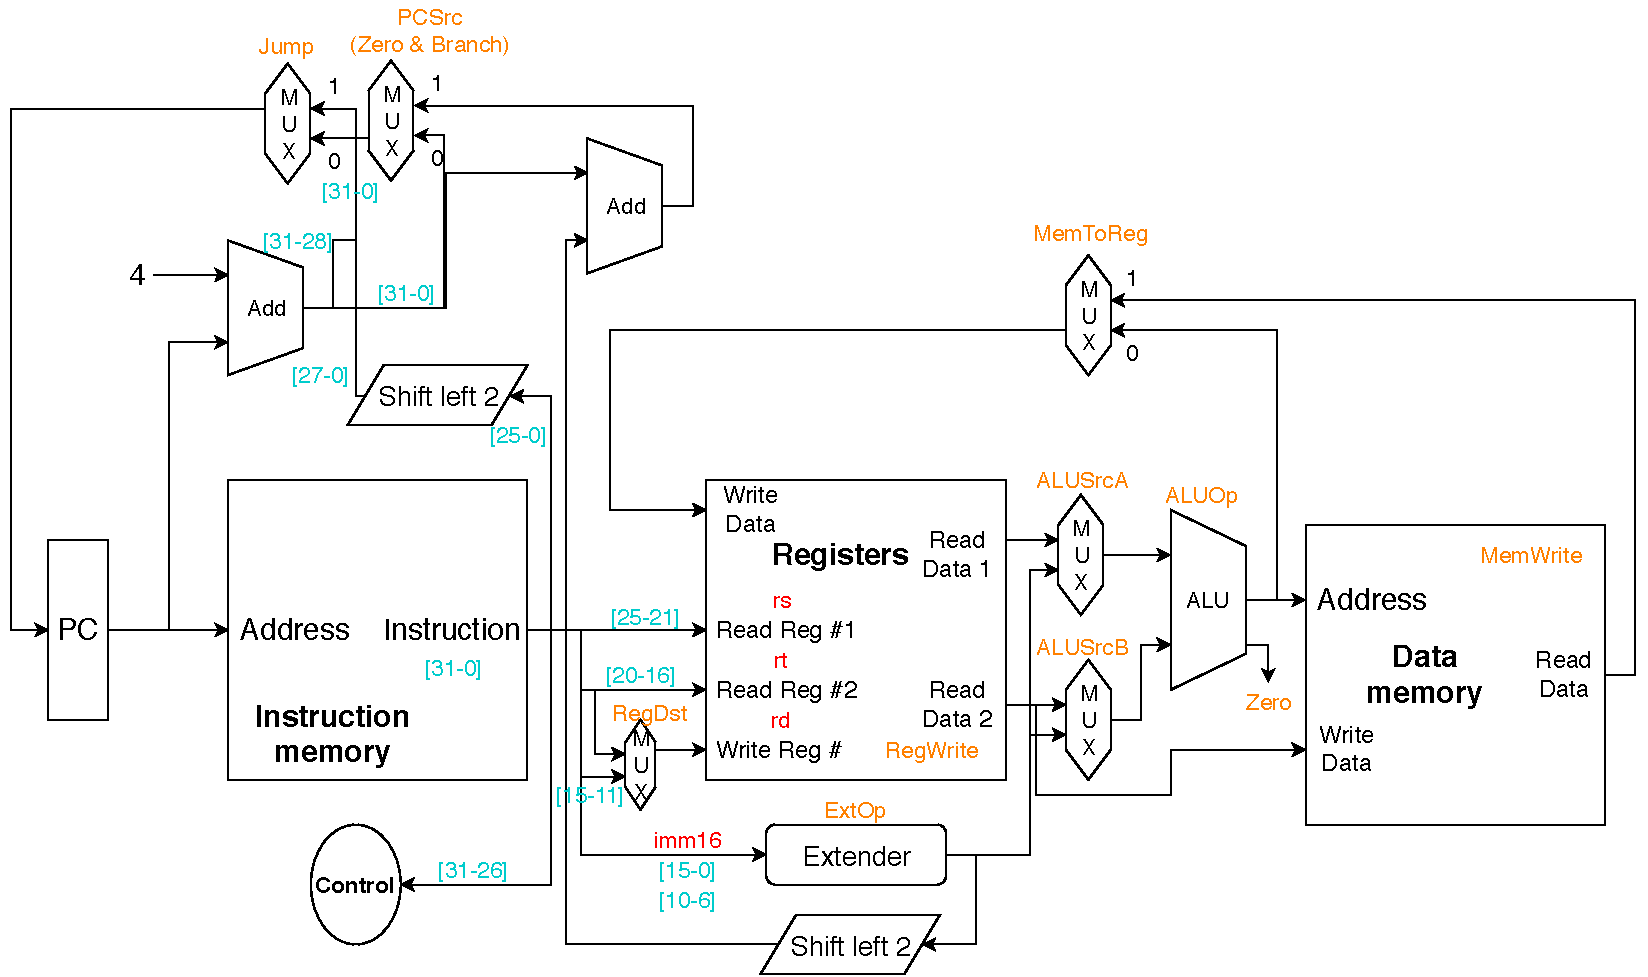
\includegraphics[width=\linewidth]{fig/Datapath.pdf}
\caption{基本数据通路}
\label{fig:datapath}
\end{figure}
\begin{table}[H]
  \centering\xiaowu
  \caption{控制信号}
    \begin{tabular}{|l|l|l|}
    \hline
    \multicolumn{1}{|c|}{控制信号名} & \multicolumn{1}{c|}{状态0} & \multicolumn{1}{c|}{状态1} \bigstrut\\
    \hline
    Reset & 初始化PC为0 & PC接收新地址 \bigstrut\\
    \hline
    PCWre & PC不更改,halt & PC更改 \bigstrut\\
    \hline
    RegDst & 写入寄存器地址来自rt字段 & 写入寄存器地址来自rd字段 \bigstrut\\
    \hline
    RegWrite & 寄存器不可写 & 寄存器可写 \bigstrut\\
    \hline
    ALUSrcA & 寄存器rs内容 & 立即数sa \bigstrut\\
    \hline
    ALUSrcB & 寄存器rt内容 & 立即数imm \bigstrut\\
    \hline
    ExtOp & 零扩展   & 符号扩展 \bigstrut\\
    \hline
    ALUOp & \multicolumn{2}{c|}{见表\ref{tab:alu_op}} \bigstrut\\
    \hline
    MemToReg & ALU输出 & 内存读取 \bigstrut\\
    \hline
    MemWrite & 内存不可写 & 内存可写 \bigstrut\\
    \hline
    Branch & 非分支   & 分支 \bigstrut\\
    \hline
    Jump  & 非跳转   & 跳转 \bigstrut\\
    \hline
    \end{tabular}%
  \label{tab:control}%
\end{table}%

\subsubsection{MIPS指令格式}
\qquad MIPS指令可分为以下三种格式,见图\ref{fig:mips_type}。
\begin{figure}[htbp]
\centering
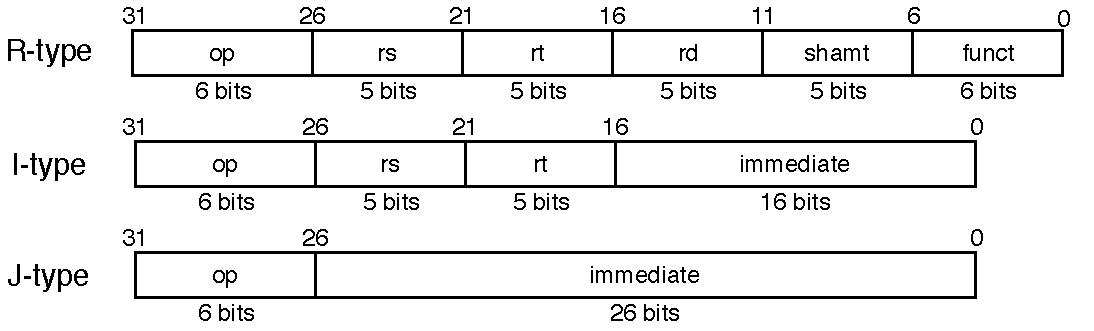
\includegraphics[width=0.8\linewidth]{fig/MIPS.pdf}
\caption{MIPS指令类型}
\label{fig:mips_type}
\end{figure}
其中各字段缩写含义如表\ref{tab:mips}所示。
% Table generated by Excel2LaTeX from sheet 'Sheet1'
\begin{table}[htbp]
  \centering\xiaowu
  \caption{\xiaowu MIPS指令各字段缩写含义}
    \begin{tabular}{|l|l|}
    \hline
    op    & 操作码 \bigstrut\\
    \hline
    rs    & 只读,第一个源操作数寄存器地址/编号,范围为\verb'0x00'$\sim$\verb'0x1F' \bigstrut\\
    \hline
    rt    & 可读可写,第二个源操作数地址或目标操作数寄存器地址 \bigstrut\\
    \hline
    rd    & 只写,目的操作数寄存器地址 \bigstrut\\
    \hline
    sham(shift amt) & 位移量,在移位指令中用于指定移多少位 \bigstrut\\
    \hline
    funct & 功能码,在R类型指令中配合op一起使用 \bigstrut\\
    \hline
    immediate & 16位立即数 \bigstrut\\
    \hline
    address & 目标转移地址 \bigstrut\\
    \hline
    \end{tabular}%
  \label{tab:mips}%
\end{table}%
% !TEX root = main.tex

\subsection{各指令数据通路分析}
\qquad公共的数据通路为取指和PC+4,见图\ref{fig:datapath_add}最左红色通路,下文将不再提及。
\subsubsection{算术逻辑运算}
\begin{enumerate}
	\item add/sub/and/or指令均为R类型,数据通路相同,唯一不同为ALU操作码的选择。见图\ref{fig:datapath_add},执行阶段从指令中读入rs、rt、rd三个寄存器的地址,然后从寄存器堆中读出rs和rt寄存器的内容,送至ALU进行运算,最后写回rd寄存器。
	\item addiu/andi/ori/slti指令均为I类型,数据通路相同,同样是ALU操作码不同。见图\ref{fig:datapath_addi},执行阶段从指令中读入rs、rt寄存器的地址,但rt是作为写入寄存器(RegDst=0);指令低16位进行扩充,将rs的内容和立即数送入ALU运算,最后写回rt寄存器。注意addiu/slti进行\textbf{符号}扩展,andi/ori进行零扩展。
	\item sll指令为R类型,但是指令格式比较特殊。见图\ref{fig:datapath_sll},执行阶段从指令中读入rt寄存器的地址并取出,取指令的[10:6]位读出立即数sa并进行零扩展(ALUSrcA=1),利用ALU对rt的内容及sa进行移位操作,结果写回rd寄存器。
\end{enumerate}
\begin{figure}[htbp]
\centering
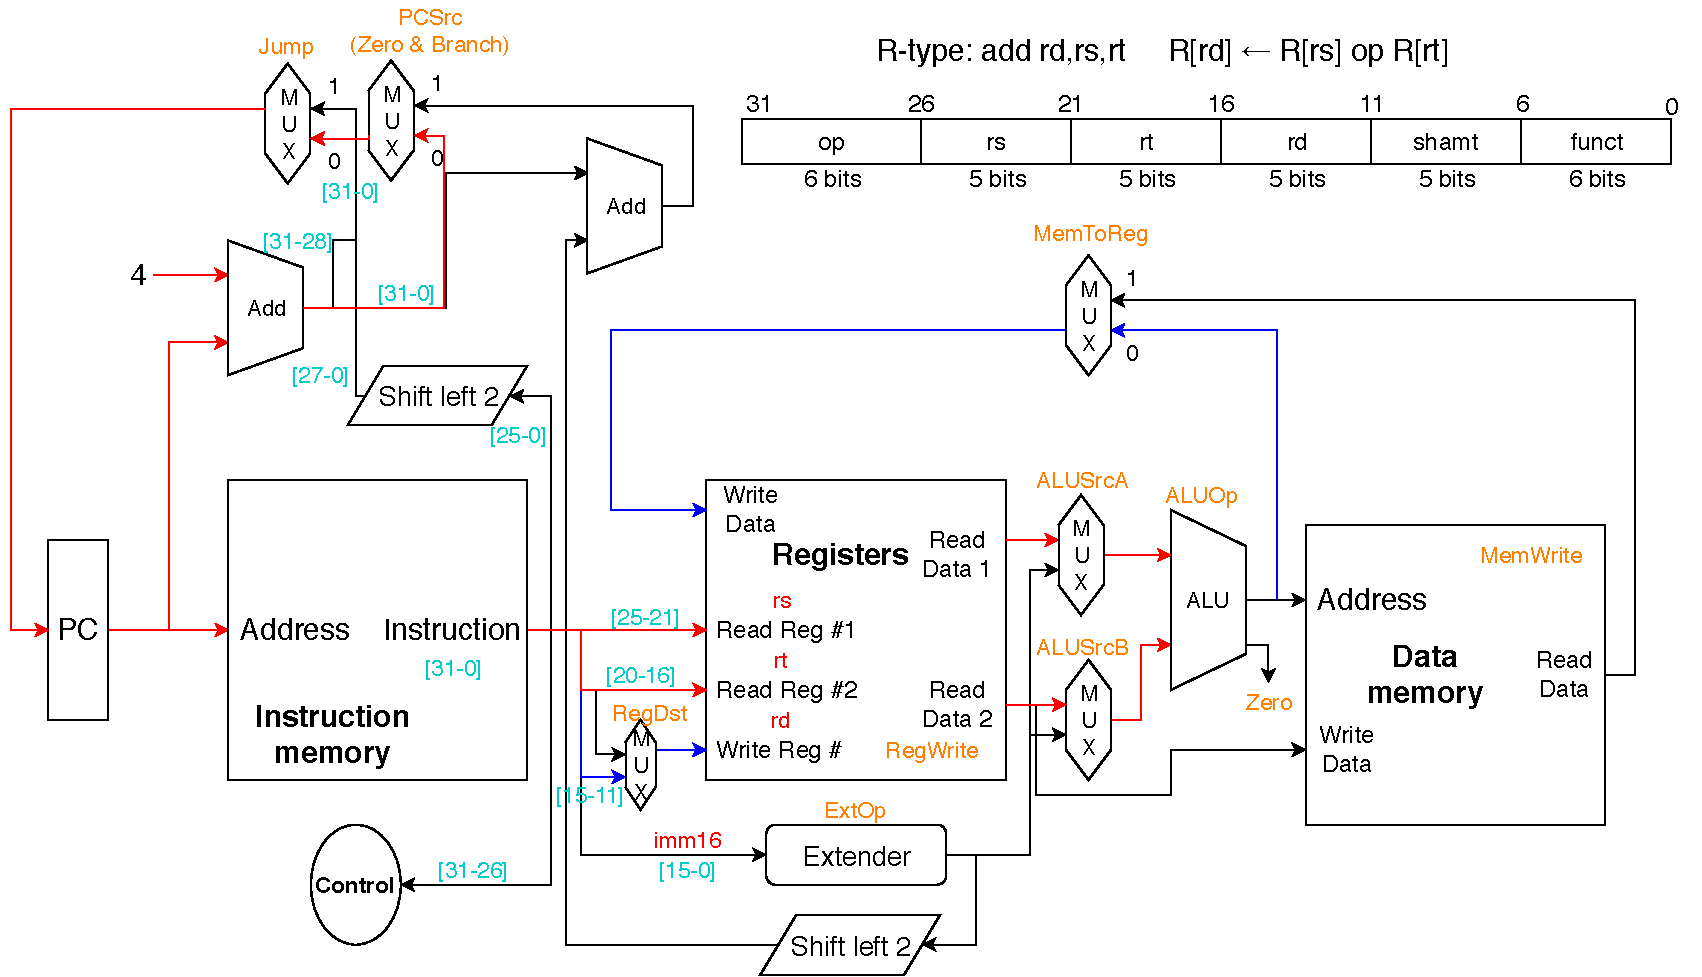
\includegraphics[width=\linewidth]{fig/Datapath_add.pdf}
\caption{Add/sub/and/or通路}
\label{fig:datapath_add}
\end{figure}
\begin{figure}[htbp]
\centering
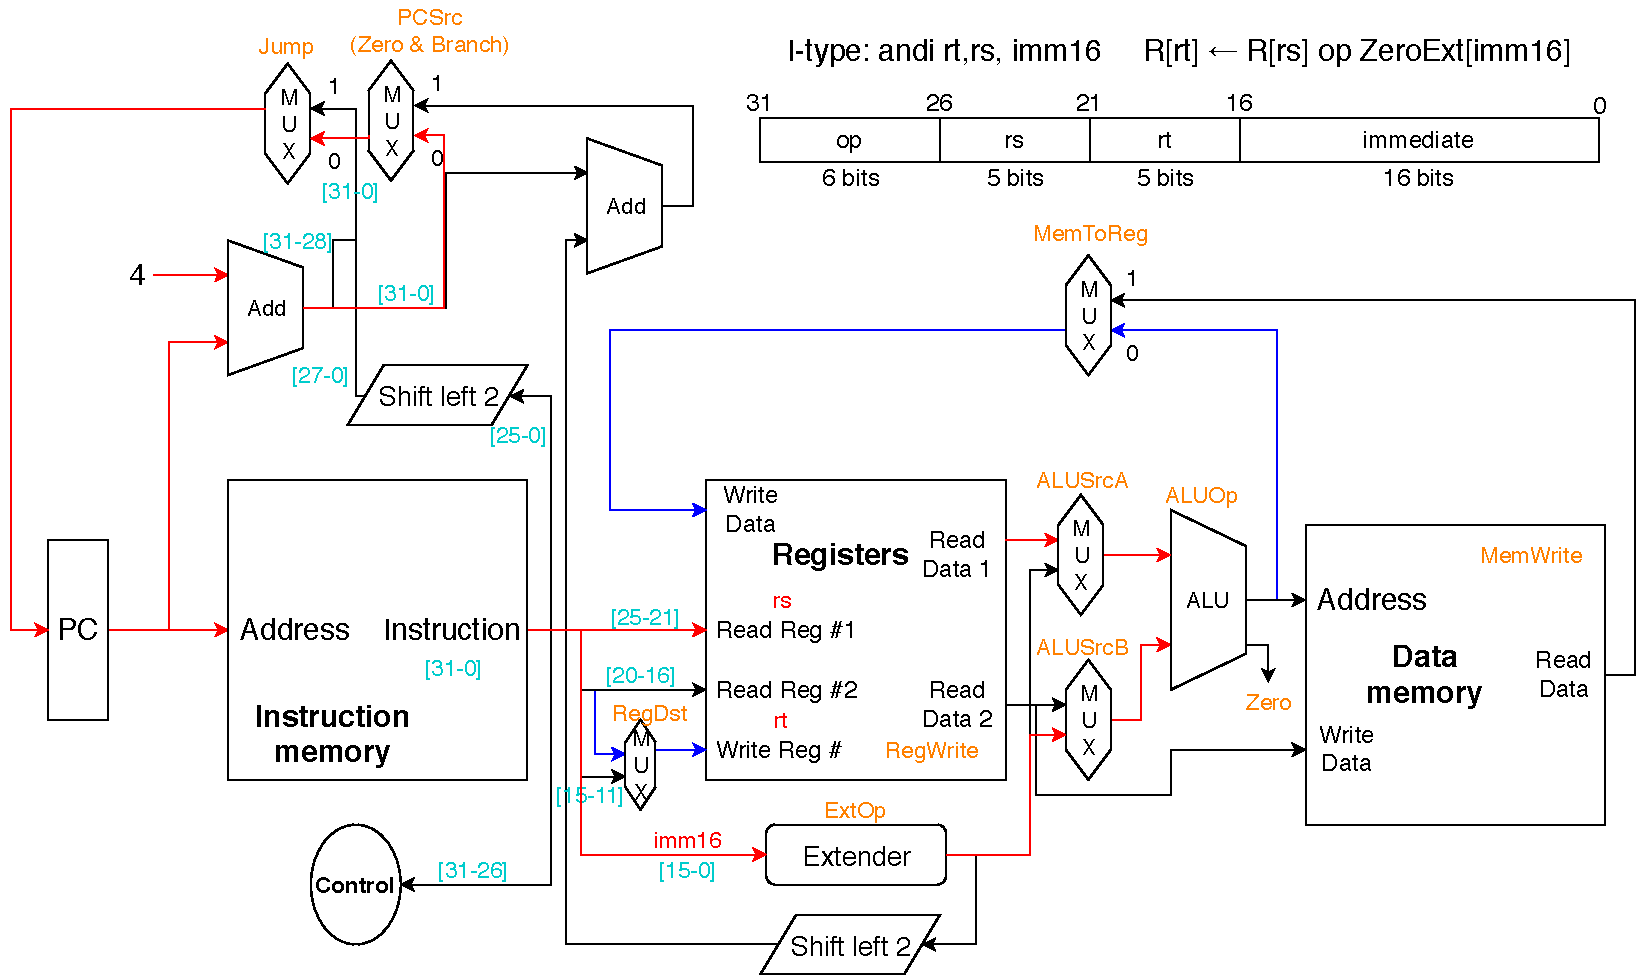
\includegraphics[width=\linewidth]{fig/Datapath_addi.pdf}
\caption{Addiu/andi/ori/slti通路}
\label{fig:datapath_addi}
\end{figure}
\begin{figure}[htbp]
\centering
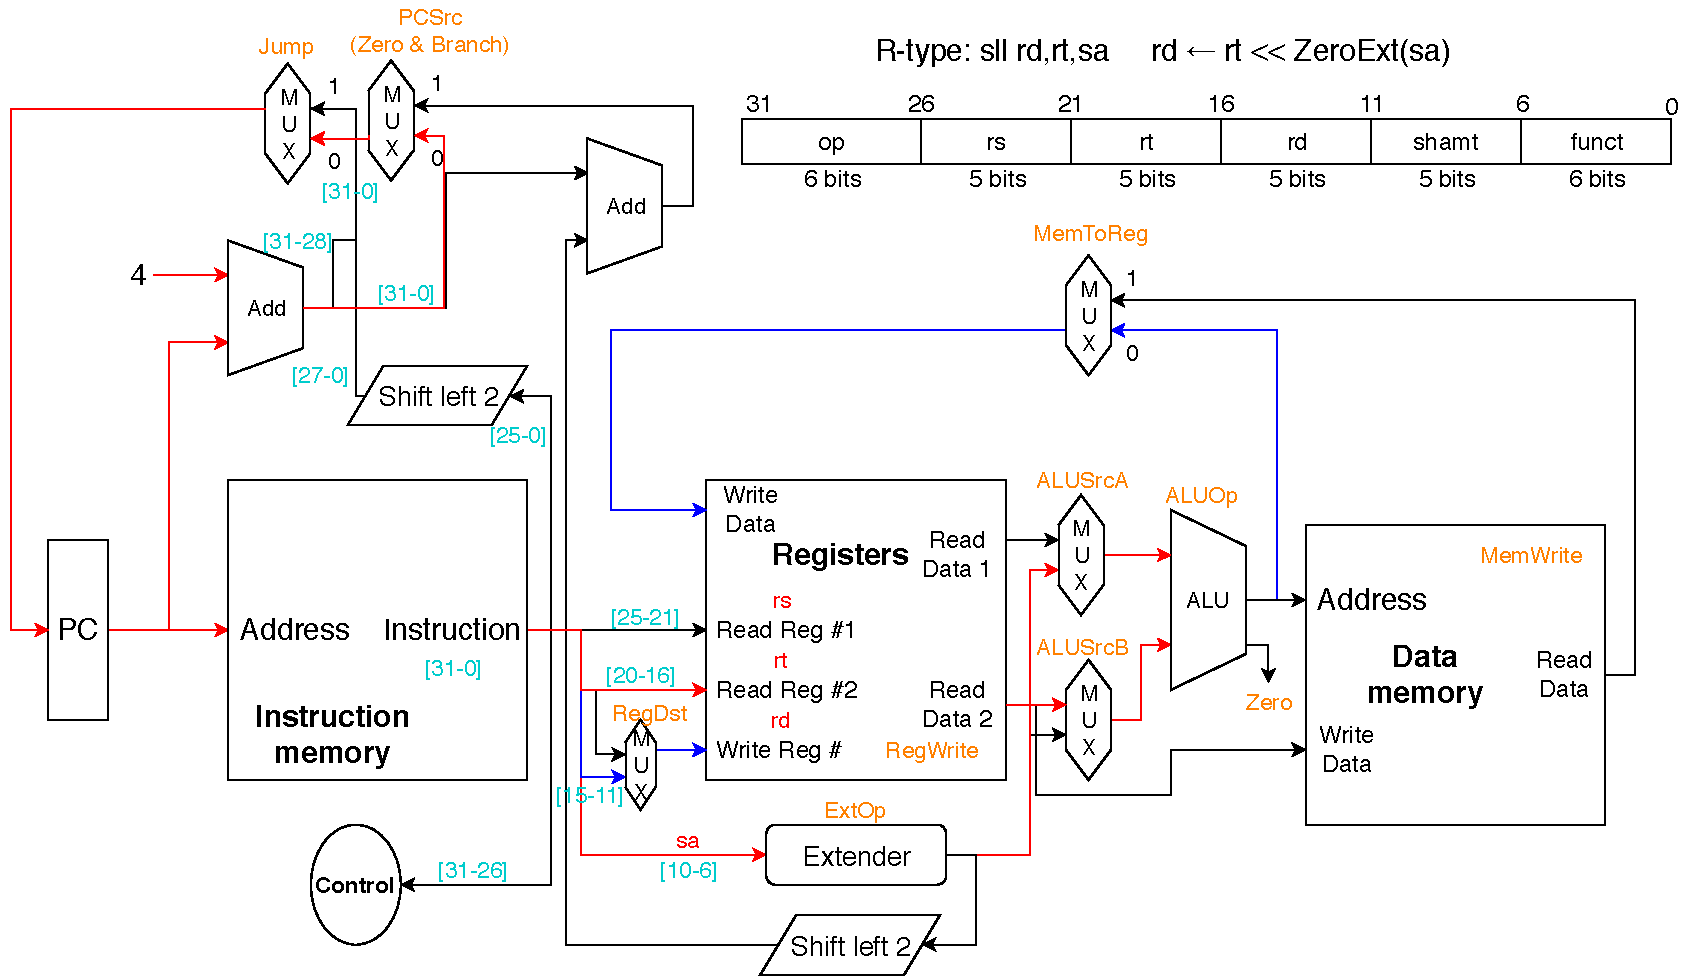
\includegraphics[width=\linewidth]{fig/Datapath_sll.pdf}
\caption{sll通路}
\label{fig:datapath_sll}
\end{figure}

\subsubsection{访存}
\begin{enumerate}
	\item sw为I类型。见图\ref{fig:datapath_sw},执行阶段从指令中读入rs、rt寄存器的地址,对偏移量(imm)进行\textbf{符号}扩展,与rs寄存器的内容相加得到内存地址,将rt寄存器的内容写入内存。
	\item lw为I类型。见图\ref{fig:datapath_lw},执行阶段从指令中读入rs、rt寄存器的地址,rt作为写入寄存器(RegDst=0),对偏移量(imm)进行\textbf{符号}扩展,与rs寄存器的内容相加得到内存地址,将内存的内容写入rt寄存器。
\end{enumerate}
\begin{figure}[htbp]
\centering
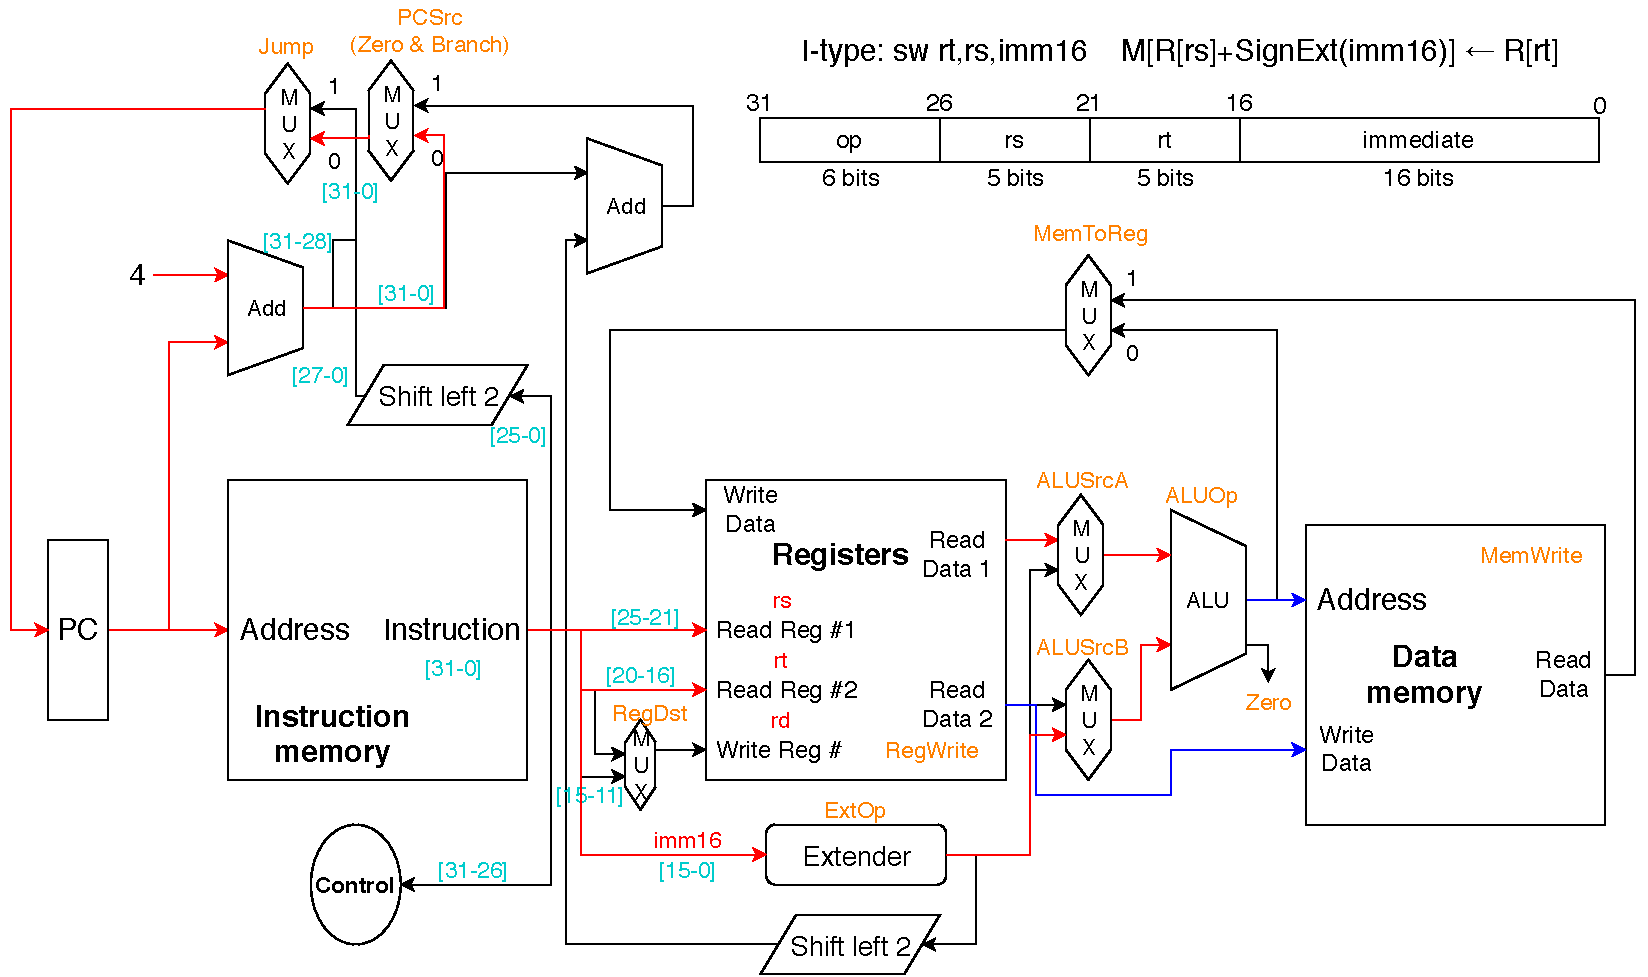
\includegraphics[width=\linewidth]{fig/Datapath_sw.pdf}
\caption{sw通路}
\label{fig:datapath_sw}
\end{figure}
\begin{figure}[htbp]
\centering
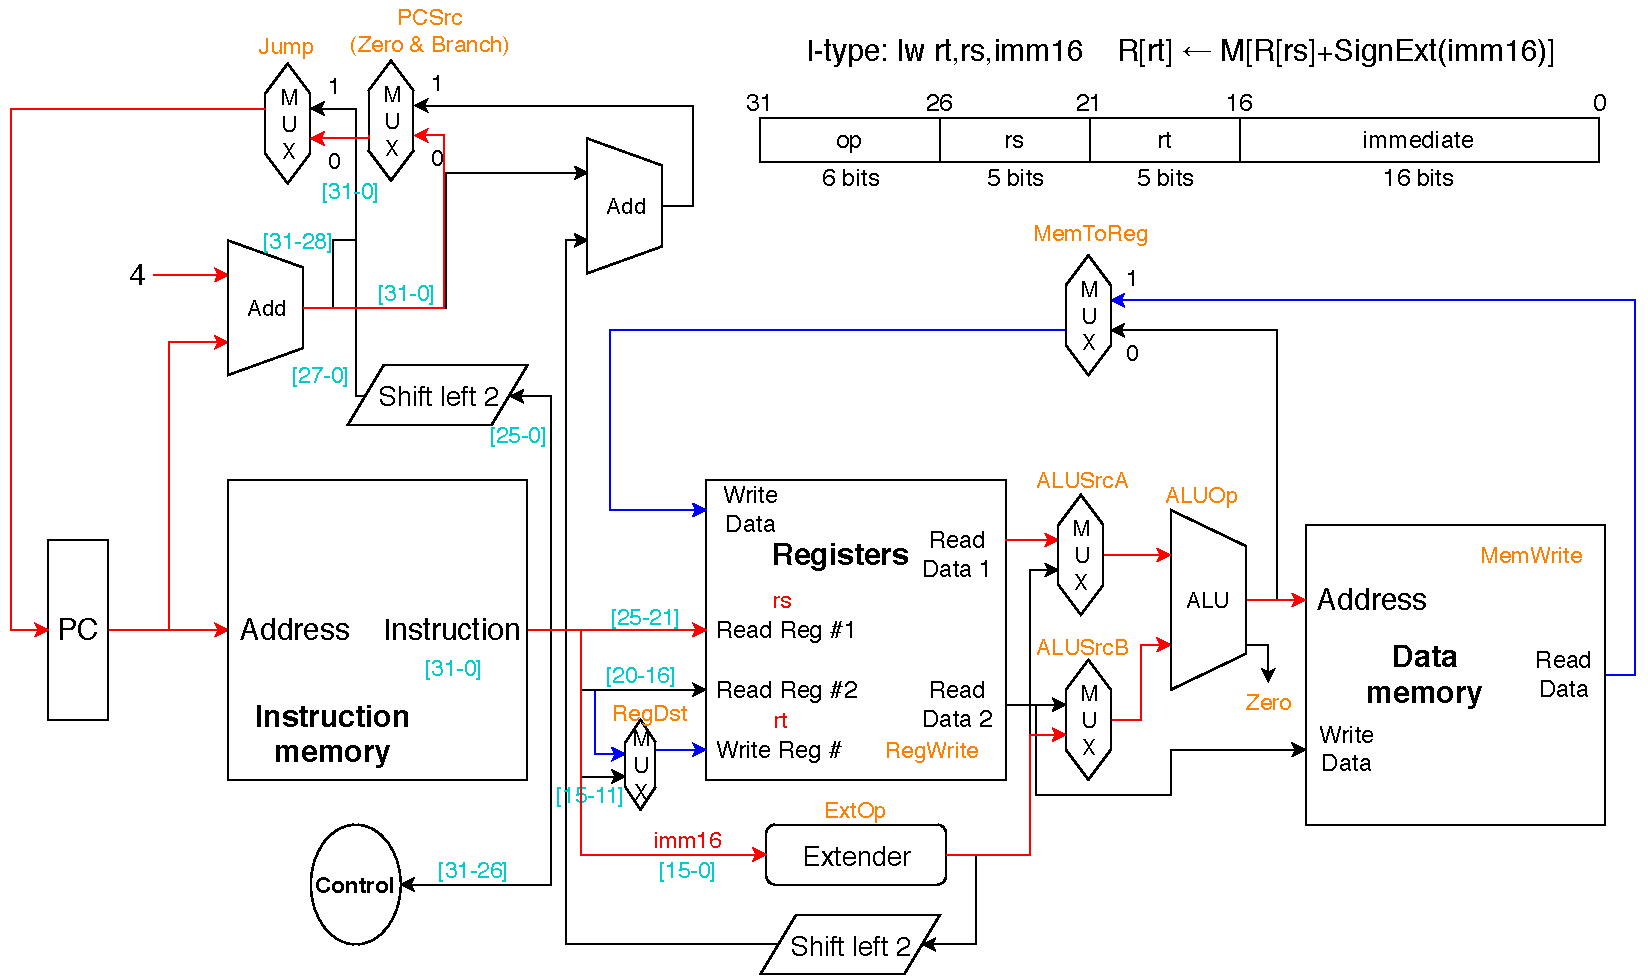
\includegraphics[width=\linewidth]{fig/Datapath_lw.pdf}
\caption{lw通路}
\label{fig:datapath_lw}
\end{figure}

\subsubsection{分支跳转}
\qquad由于MIPS指令为32位(4字节),一般情况下PC每次自增都加4,即PC末两位一定为0,放在指令中(PC偏移/转移地址)即可省略末两位。指令读出时则要左移2位,将末尾的0补齐。
为最大程度利用指令的每一位,跳转指令也是将高4位和低2位都省略掉了,读出时要补回。
\begin{enumerate}
	\item beq/bne/bltz为I类型。见图\ref{fig:datapath_beq},执行阶段从指令中读入rs、rt寄存器的地址,利用ALU对rs、rt寄存器的内容进行相减(beq/bne)或有符号比较(bltz),若结果为0,则Zero标志置1,否则置0;同时,立即数imm进行符号扩展,并左移两位,与原有的PC+4再相加,得到是否执行分支跳转指令(beq: PCSrc=Zero, bne/bltz: PCSrc=$\sim$Zero)。
	\item jump为j类型。见图\ref{fig:datapath_jump},执行阶段直接对指令的低26位左移2位,补上PC+4的高4位,得到跳转地址,更新PC。
\end{enumerate}
\begin{figure}[htbp]
\centering
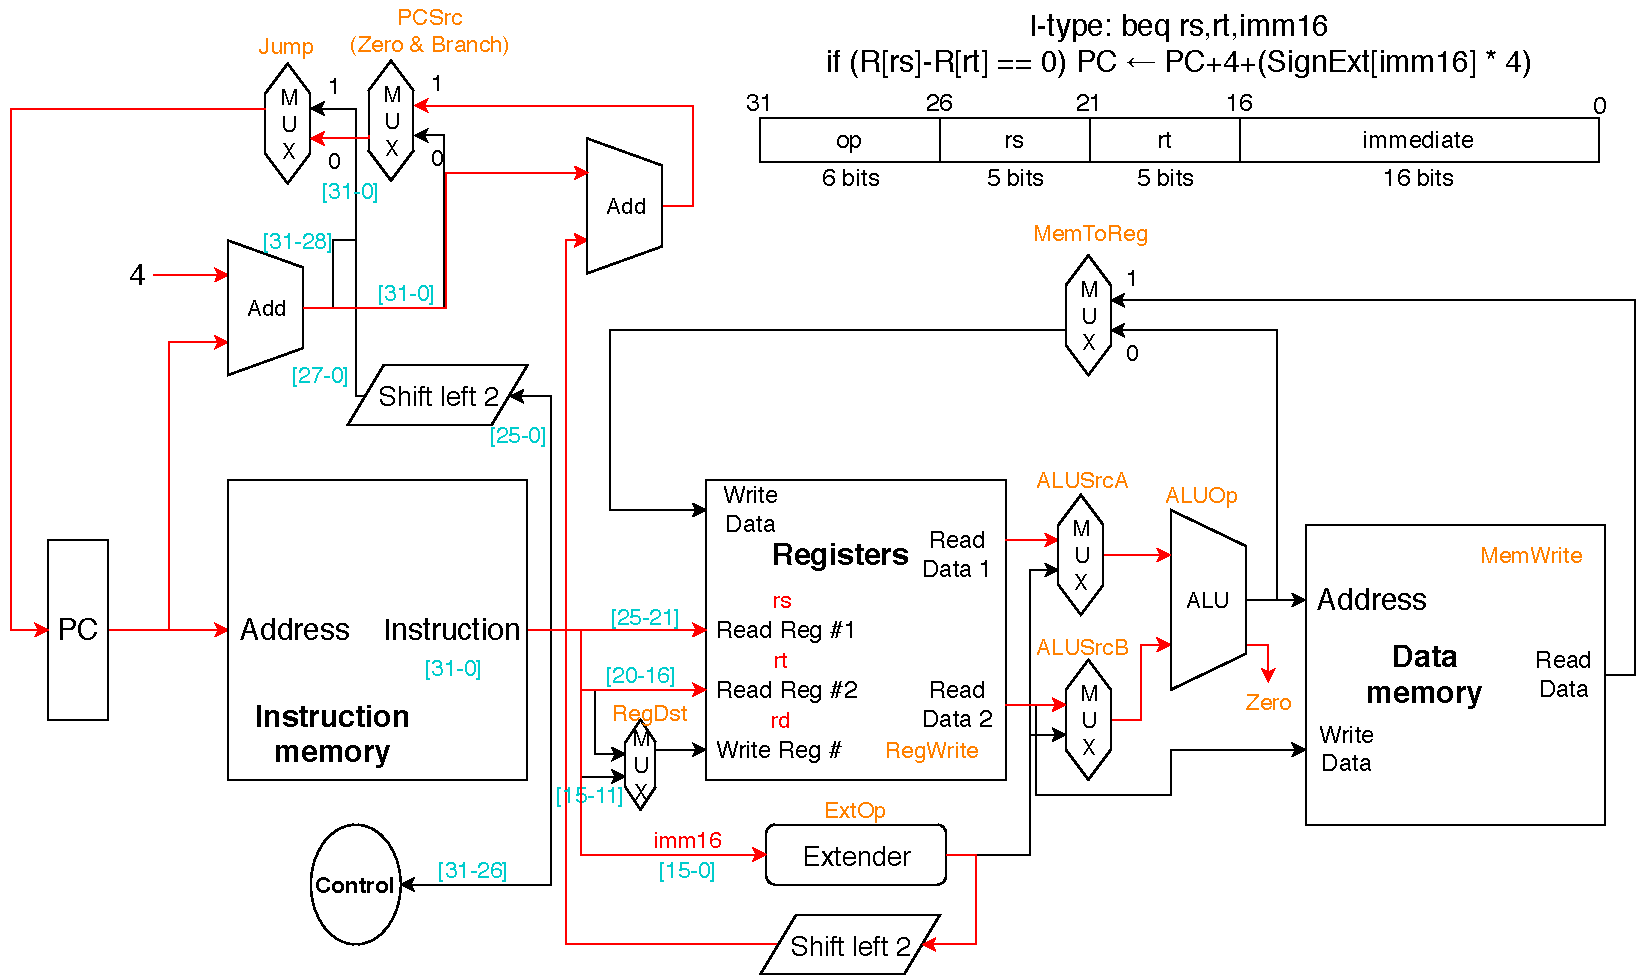
\includegraphics[width=\linewidth]{fig/Datapath_beq.pdf}
\caption{beq/bne/bltz通路}
\label{fig:datapath_beq}
\end{figure}
\begin{figure}[htbp]
\centering
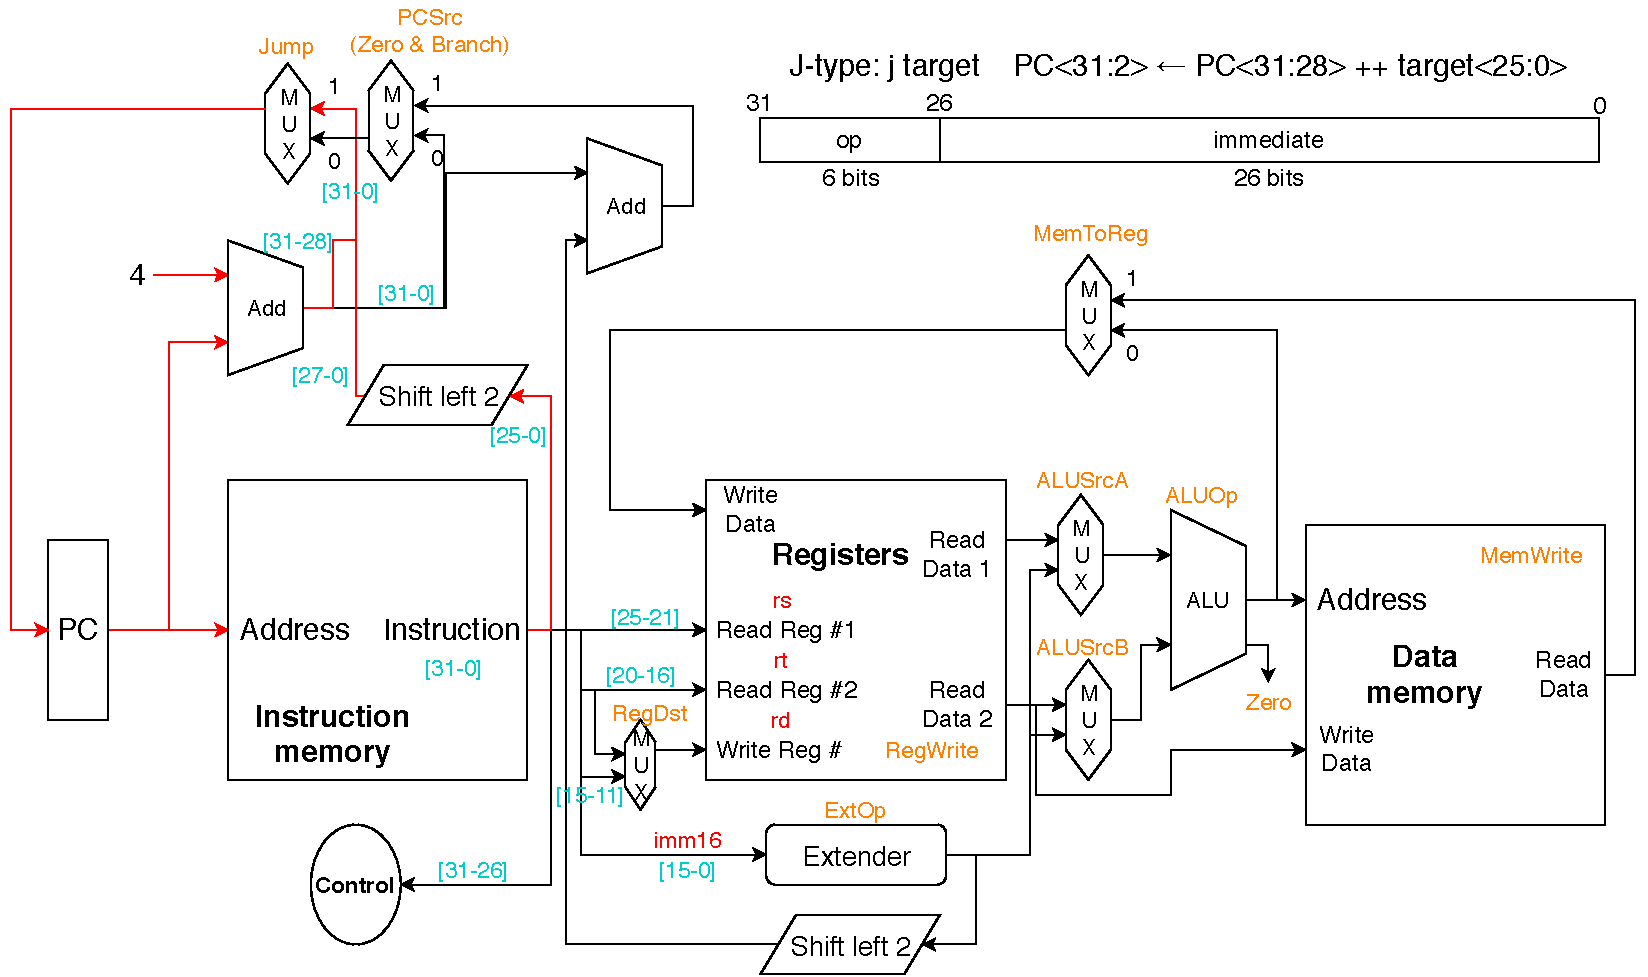
\includegraphics[width=\linewidth]{fig/Datapath_jump.pdf}
\caption{jump通路}
\label{fig:datapath_jump}
\end{figure}

\subsubsection{停机指令}
\qquad PCWrite置为0,不改变PC的值,PC不再变化
% !TEX root = main.tex

\subsection{各组件实现}
\qquad 各组件实现详情见第\ref{sec:appendix}章节,均有详细注释。在这里仅仅提一些需要注意的点。
\begin{enumerate}
	\item 指令存储器和数据存储器均采用小端(little endian)存储,并且位宽为8位,故生成的指令文件需要进行预处理,最先读入的应该是指令的低8位。这里用\verb'Python'进行MIPS程序的编译并生成指令二进制代码文件,读入时直接将其初始化到指令存储器中。
	\item 程序计数器(PC)需要初始化置零(\verb'0x000000'),遇到reset信号时同样置零,而且只有在PCWrite=1时才更新PC。
	\item 多路选择器(MUX)需要实现一个32位和一个5位的,32位可以复用(创建多个实例);且需要构造2输入、3输入、4输入三种不同的MUX。
	\item ALU的功能见表\ref{tab:alu_op}。
    \item 控制单元的设计见第\ref{sub:control_unit}节。
\end{enumerate}
% Table generated by Excel2LaTeX from sheet 'ALUOp'
\begin{table}[htbp]
  \centering\xiaowu
  \caption{ALU功能码}
    \begin{tabular}{|c|l|l|}
    \hline
    ALUOp[2:0] & \multicolumn{1}{c|}{功能} & \multicolumn{1}{c|}{描述} \\
    \hline
    000   & $Y=A+B$ & 加 \\
    \hline
    001   & $Y=A-B$ & 减 \\
    \hline
    010   & $Y=B<<A$ & 左移 \\
    \hline
    011   & $Y=A\lor B$ & 逻辑或 \\
    \hline
    100   & $Y=A\land B$ & 逻辑与 \\
    \hline
    101   & $Y=(A<B)\;?\;1\;:\;0$ & 比较无符号数 \\
    \hline
    110   & \multicolumn{1}{p{7cm}|}{$\begin{aligned}
    Y&=(((A<B) \&\& (A[31] == B[31] ))\\
    &||\quad( ( A[31] ==1 \&\& B[31] == 0)))\\
    &?\;1\;:\;0
    \end{aligned}$} & 比较有符号数 \\
    \hline
    111   & $Y=A\oplus B$ & 逻辑异或 \\
    \hline
    \end{tabular}%
  \label{tab:alu_op}%
\end{table}%
% !TEX root = main.tex

\subsection{控制单元}
\label{sub:control_unit}
\qquad 由前面的分析,可以得到控制单元的编码表,见表\ref{tab:control_codes}。
% Table generated by Excel2LaTeX from sheet 'TrueTable'
\begin{sidewaystable}[htbp]
  \centering\xiaowu
  \caption{指令控制器编码}
    \begin{tabular}{|c|l|l|r|r|r|p{1cm}|p{1cm}|r|r|r|r|r|}
    \hline
          & \multicolumn{1}{c|}{指令} & \multicolumn{1}{c|}{op} & \multicolumn{1}{c|}{RegDst} & \multicolumn{1}{c|}{ExtSel} & \multicolumn{1}{c|}{RegWrite} & \multicolumn{2}{c|}{ALUSrcA/B} & \multicolumn{1}{c|}{ALUOp} & \multicolumn{1}{c|}{MemToReg} & \multicolumn{1}{c|}{MemWrite} & \multicolumn{1}{c|}{Branch} & \multicolumn{1}{c|}{Jump} \bigstrut\\
    \hline
    \multirow{3}[6]{*}{算术运算} & add rd, rs, rt & 000000 & 1     & x     & 1     & 0     & 0     & 000   & 0     & 0     & 0     & 0 \bigstrut\\
\cline{2-13}          & sub rd, rs, rt & 000001 & 1     & x     & 1     & 0     & 0     & 001   & 0     & 0     & 0     & 0 \bigstrut\\
\cline{2-13}          & addiu rt, rs, imm & 000010 & 0     & \textbf{1} & 1     & 0     & 1     & 000   & 0     & 0     & 0     & 0 \bigstrut\\
    \hline
    \multirow{4}[8]{*}{逻辑运算} & andi rt, rs, imm & 010000 & 0     & 0     & 1     & 0     & 1     & 100   & 0     & 0     & 0     & 0 \bigstrut\\
\cline{2-13}          & and rd, rs, rt & 010001 & 1     & x     & 1     & 0     & 0     & 100   & 0     & 0     & 0     & 0 \bigstrut\\
\cline{2-13}          & ori rt, rs, imm & 010010 & 0     & 0     & 1     & 0     & 1     & 011   & 0     & 0     & 0     & 0 \bigstrut\\
\cline{2-13}          & or rd, rs, rt & 010011 & 1     & x     & 1     & 0     & 0     & 011   & 0     & 0     & 0     & 0 \bigstrut\\
    \hline
    移位    & sll rd, rt, sa & 011000 & 1     & x     & 1     & 1     & 0     & 010   & 0     & 0     & 0     & 0 \bigstrut\\
    \hline
    比较    & slti rt, rs, imm & 011100 & 0     & 1     & 1     & 0     & 1     & 110   & 0     & 0     & 0     & 0 \bigstrut\\
    \hline
    \multirow{2}[4]{*}{访存} & sw rt, imm(rs) & 100110 & x     & 1     & 0     & 0     & 1     & 000   & x     & 1     & 0     & 0 \bigstrut\\
\cline{2-13}          & lw rt, imm(rs) & 100111 & 0     & 1     & 1     & 0     & 1     & 000   & 1     & 0     & 0     & 0 \bigstrut\\
    \hline
    \multirow{3}[6]{*}{分支} & beq rs, rt, imm & 110000 & x     & 1     & 0     & 0     & 0     & 001   & x     & 0     & 1     & 0 \bigstrut\\
\cline{2-13}          & bne rs, rt, imm & 110001 & x     & 1     & 0     & 0     & 0     & 001   & x     & 0     & 1     & 0 \bigstrut\\
\cline{2-13}          & bltz rs, imm & 110010 & x     & 1     & 0     & 0     & 0     & 110   & x     & 0     & 1     & 0 \bigstrut\\
    \hline
    跳转    & j addr & 111000 & x     & x     & 0     & x     & x     & x     & x     & 0     & 0     & 1 \bigstrut\\
    \hline
    停机    & halt  & 111111 & x     & x     & x     & x     & x     & x     & x     & x     & x     & x \bigstrut\\
    \hline
    \end{tabular}%
  \label{tab:control_codes}%
\end{sidewaystable}%


\section{实验步骤}
% !TEX root = main.tex

\subsection{简易编译器}
\qquad 本次实验用\verb'Python'写了一个简单的编译器来实现MIPS代码到二进制代码的转换。主要采用正则表达式库(\verb're')对输入的字符串进行处理。基本实现思路如下:
\begin{enumerate}
    \item 逐行读入汇编源文件,遇到非指令行(如注释)则直接丢弃,其余行送入\verb'parse'函数。
    \item 在\verb'parse'函数内判断指令名称,并依据不同的指令格式分别进行字符串的分割和处理,这里采用了正则表达式进行分割。
    \item 将操作、寄存器编号、立即数等全部转化为二进制。不够位数的用0补足,负数要用补码表示。
    \item 将这些二进制数连接起来,得到32位的二进制字符串,返回
    \item 逐行输出二进制编码和十六进制编码,并写入文件,注意这里采用小端存储(每8位作为一个字节/单位)
\end{enumerate}
\par 完整程序附在第\ref{sec:appendix}章编译器一节。
% !TEX root = main.tex

\subsection{仿真模拟}
\qquad 采用表\ref{tab:test}给出的汇编程序代码段进行测试。注意指令的二进制编码应该对应到MIPS的每一个字段上,特别注意sll的书写,负数用补码表示等。生成二进制指令文件后,CPU将其读入指令存储器并执行,看波形结果。
% Table generated by Excel2LaTeX from sheet 'TrueTable'
\begin{table}[htbp]
  \centering\xiaowu
  \caption{测试代码段指令}
    \begin{tabular}{|l|l|l|l|l|llll|l|}
    \hline
    \multicolumn{1}{|c|}{address} & \multicolumn{1}{c|}{instruction} & \multicolumn{1}{c|}{op} & \multicolumn{1}{c|}{rs} & \multicolumn{1}{c|}{rt} & \multicolumn{4}{c|}{rd/imm}   & \multicolumn{1}{c|}{hex} \bigstrut\\
    \hline
    0x00000000 & addiu  \$1,\$0,8 & 000010 & 00000 & 00001 & 0000  & 0000  & 0000  & 1000  & 0x08010008 \bigstrut\\
    \hline
    0x00000004 & ori  \$2,\$0,2 & 010010 & 00000 & 00010 & 0000  & 0000  & 0000  & 0010  & 0x48020002 \bigstrut\\
    \hline
    0x00000008 & xori  \$3,\$2,8 & 010011 & 00010 & 00011 & 0000  & 0000  & 0000  & 1000  & 0x4c430008 \bigstrut\\
    \hline
    0x0000000C & sub  \$4,\$3,\$1 & 000001 & 00011 & 00001 & 0010  & 0000  & 0000  & 0000  & 0x04612000 \bigstrut\\
    \hline
    0x00000010 & and  \$5,\$4,\$2 & 010000 & 00100 & 00010 & 0010  & 1000  & 0000  & 0000  & 0x40822800 \bigstrut\\
    \hline
    0x00000014 & sll   \$5,\$5,2 & 011000 & 00000 & 00101 & 0010  & 1000  & 1000  & 0000  & 0x60052880 \bigstrut\\
    \hline
    0x00000018 & beq  \$5,\$1,-2(=,转14) & 110100 & 00101 & 00001 & 1111  & 1111  & 1111  & 1110  & 0xd0a1fffe \bigstrut\\
    \hline
    0x0000001C & jal  0x0000050 & 111010 & 00000 & 00000 & 0000  & 0000  & 0001  & 0100  & 0xe8000014 \bigstrut\\
    \hline
    0x00000020 & slt  \$8,\$13,\$1 & 100111 & 01101 & 00001 & 0100  & 0000  & 0000  & 0000  & 0x9da14000 \bigstrut\\
    \hline
    0x00000024 & addiu  \$14,\$0,-2 & 000010 & 00000 & 01110 & 1111  & 1111  & 1111  & 1110  & 0x080efffe \bigstrut\\
    \hline
    0x00000028 & slt  \$9,\$8,\$14 & 100111 & 01000 & 01110 & 0100  & 1000  & 0000  & 0000  & 0x9d0e4800 \bigstrut\\
    \hline
    0x0000002C & slti  \$10,\$9,2 & 100110 & 01001 & 01010 & 0000  & 0000  & 0000  & 0010  & 0x992a0002 \bigstrut\\
    \hline
    0x00000030 & slti  \$11,\$10,0 & 100110 & 01010 & 01011 & 0000  & 0000  & 0000  & 0000  & 0x994b0000 \bigstrut\\
    \hline
    0x00000034 & add  \$11,\$11,\$10 & 000000 & 01011 & 01010 & 0101  & 1000  & 0000  & 0000  & 0x016a5800 \bigstrut\\
    \hline
    0x00000038 & bne  \$11,\$2,-2 (≠,转34) & 110101 & 01011 & 00010 & 1111  & 1111  & 1111  & 1110  & 0xd562fffe \bigstrut\\
    \hline
    0x0000003C & addiu  \$12,\$0,-2 & 000010 & 00000 & 01100 & 1111  & 1111  & 1111  & 1110  & 0x080cfffe \bigstrut\\
    \hline
    0x00000040 & addiu  \$12,\$12,1 & 000010 & 01100 & 01100 & 0000  & 0000  & 0000  & 0001  & 0x098c0001 \bigstrut\\
    \hline
    0x00000044 & bltz  \$12,-2 (<0,转40) & 110110 & 01100 & 00000 & 1111  & 1111  & 1111  & 1110  & 0xd980fffe \bigstrut\\
    \hline
    0x00000048 & andi  \$12,\$2,2 & 010001 & 00010 & 01100 & 0000  & 0000  & 0000  & 0010  & 0x444c0002 \bigstrut\\
    \hline
    0x0000004C & j  0x000005C & 111000 & 00000 & 00000 & 0000  & 0000  & 0001  & 0111  & 0xe0000017 \bigstrut\\
    \hline
    0x00000050 & sw  \$2,4(\$1) & 110000 & 00001 & 00010 & 0000  & 0000  & 0000  & 0100  & 0xc0220004 \bigstrut\\
    \hline
    0x00000054 & lw  \$13,4(\$1) & 110001 & 00001 & 01101 & 0000  & 0000  & 0000  & 0100  & 0xc42d0004 \bigstrut\\
    \hline
    0x00000058 & jr  \$31 & 111001 & 11111 & 00000 & 0000  & 0000  & 0000  & 0000  & 0xe7e00000 \bigstrut\\
    \hline
    0x0000005C & halt  & 111111 & 00000 & 00000 & 0000  & 0000  & 0000  & 0000  & 0xfc000000 \bigstrut\\
    \hline
    \end{tabular}%
  \label{tab:test}%
\end{table}%

% !TEX root = main.tex

\subsection{上板}
\qquad 使用Basys3板运行所设计的CPU时,需要通过4个七段数码管来查看当前CPU的执行情况。
\par 只考虑指令和数据的低8位,即指令存储器中的指令地址范围和数据存储器中的数据地址范围均为 \verb'0x00'$\sim$ \verb'0xFF'。
\par 通过Basys3板上的开关SW15、SW14选择七段数码管显示的内容,具体显示的功能码如表\ref{tab:seg_code}所示。
% Table generated by Excel2LaTeX from sheet 'Display'
\begin{table}[htbp]
  \centering\wuhao
  \caption{数码管显示功能码}
    \begin{tabular}{|r|r|l|l|}
    \hline
    \multicolumn{1}{|c|}{SW15} & \multicolumn{1}{c|}{SW14} & \multicolumn{1}{c|}{左边} & \multicolumn{1}{c|}{右边} \bigstrut\\
    \hline
    0     & 0     & 当前PC  & 下条PC \bigstrut\\
    \hline
    0     & 1     & rs寄存器地址 & rs寄存器数据 \bigstrut\\
    \hline
    1     & 0     & rt寄存器地址 & rt寄存器数据 \bigstrut\\
    \hline
    1     & 1     & ALU结果输出 & DB总线数据 \bigstrut\\
    \hline
    \end{tabular}%
  \label{tab:seg_code}%
\end{table}%

\subsection{七段数码管显示电路}
\qquad基本实现步骤如下:
\begin{enumerate}
    \item 对Basys3板系统时钟信号(100MHz)进行分频,使得数码管内容能够正常显示。频率不宜过快,过快会导致全部数码管显示的都是8;也不宜过慢,否则数码管会出现暂留现象,无法连续显示。在本次实现中采用10kHz的频率进行显示。
    \item 用上面得到的频率生成4进制计数器,用于产生4个数位选信号AN3-AN0。这4个数可控制哪个数码管亮,一共四组编码(1110、1101、1011、0111),每组编码中只有一位为0(亮),其余都为1(灭),在每一个位选信号到来之时更新数码管显示。其实前两步可以一并完成,见第\ref{sec:appendix}章分频计数器一节。
    \item 将从CPU接收到的相应数据转换为数码管显示信号,与位选信号一起送往数码管显示输出。
\end{enumerate}

\subsection{其他注意事项}
\begin{enumerate}
    \item 共阳极数码管\\
    Basys3板的数码管均为共阳极,故设置七段数码管和位选信号时都要考虑0为亮,1为灭。
    \item 两个时钟信号\\%https://stackoverflow.com/questions/29737369/place-30-574-poor-placement-for-routing-between-an-io-pin-and-bufg
    CPU工作时钟和Basys3板系统时钟是两个不同的时钟,但是FPGA只支持单一全局时钟,否则在routing阶段会报错
    \begin{center}\verb'Poor placement for routing between an IO pin and BUFG'\end{center}
    故需要采取其他方法。只设置全局时钟为\verb'clk',并将CPU工作时钟\verb'clk_cpu'与其同步,即在每一个\verb'clk'上升沿时,赋值\verb'in<=clk_cpu',通过下面消抖处理后,将\verb'in'作为真正的CPU工作时钟。
    \item 消抖处理\\
    如果一次触发持续一段时间不改变状态(如原状态是0,变更为1且保持100ns),则该触发是有效的人为触发,否则则视为抖动。故可以设置一个按键状态的历史记录(16位),如果连续14位都为1,则将\verb'clk_cpu'设为高电平,否则为无效触发。具体实施细节见第\ref{sec:appendix}章写板电路一节。
\end{enumerate}

\subsection{引脚分配}
\qquad见表\ref{tab:pin}。
% Table generated by Excel2LaTeX from sheet 'pin'
\begin{table}[htbp]
  \centering\wuhao
  \caption{引脚分配表}
    \begin{tabular}{|l|l|l|}
    \hline
    \multicolumn{1}{|c|}{引脚} & \multicolumn{1}{c|}{名称} & \multicolumn{1}{c|}{作用} \bigstrut\\
    \hline
    W5    & clk   & 全局时钟 \bigstrut\\
    \hline
    T17   & clk\_cpu & CPU时钟(单脉冲信号) \bigstrut\\
    \hline
    V17   & reset & 复位信号 \bigstrut\\
    \hline
    R2/T1 & SW\_in & 数码管显示内容选择 \bigstrut\\
    \hline
    W4-U2 & AN3-AN0 & 数码管位选信号 \bigstrut\\
    \hline
    W7-U7 & seg6-seg0 & 七段数码管内容 \bigstrut\\
    \hline
    \end{tabular}%
  \label{tab:pin}%
\end{table}%

\subsection{代码层次结构}
\qquad 见图\ref{fig:code_hierachy}。
\begin{figure}[H]
\centering
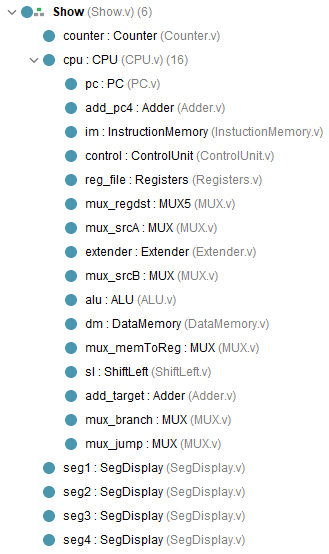
\includegraphics[width=0.4\linewidth]{fig/code_hierachy.PNG}
\caption{代码层次结构}
\label{fig:code_hierachy}
\end{figure}

\section{结果与分析}
% !TEX root = main.tex

\subsection{仿真模拟}
\qquad 设置时钟周期为100ns,初始30ns为准备时间,然后将Reset设为1使其开始工作。仿真结果见图\ref{fig:wave_1}到图\ref{fig:wave_15},每条指令的说明均已附在波形图之下。可以看见仿真结果与预期结果相同。
\begin{enumerate}
    \item \verb'0x00  addiu $1,$0,8'\\
    IF(0)状态的后半周期读入指令,并写入指令寄存器IR;WB(7)状态的后半周期将结果8写入Reg[1]
    \item \verb'0x04  ori $2,$0,2'\\
    WB(7)状态后半周期将结果2写入Reg[2]
\begin{figure}[H]
\centering
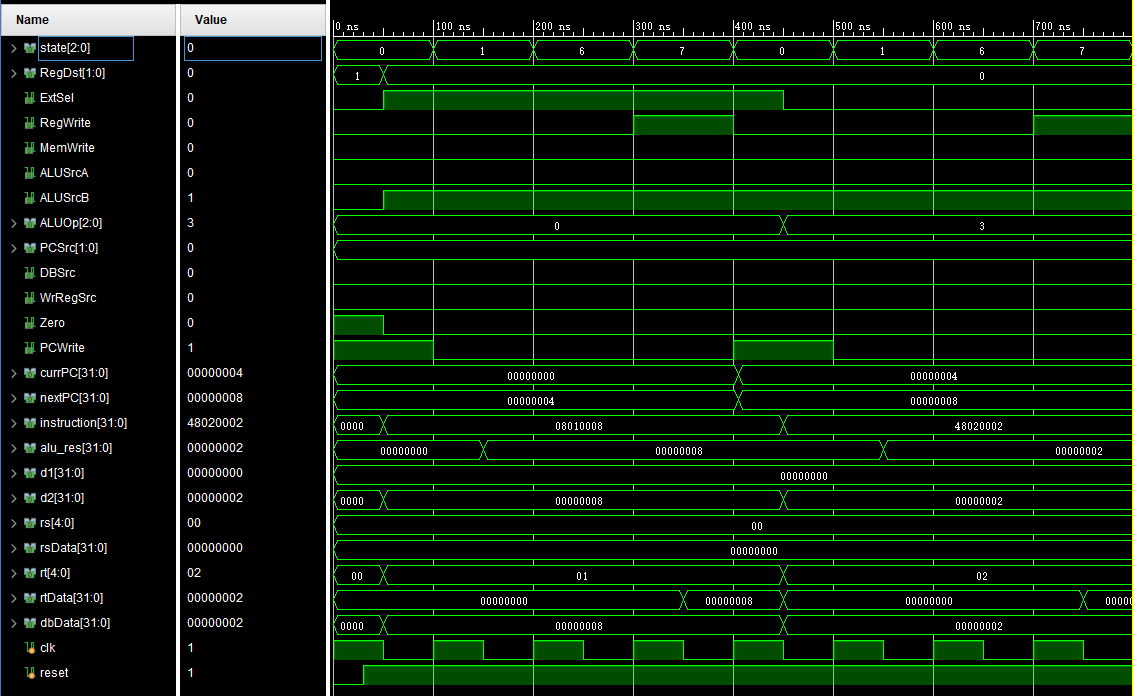
\includegraphics[width=0.9\linewidth]{fig/FullIns/Ins1.PNG}
\caption{波形图1}
\label{fig:wave_1}
\end{figure}
    \item \verb'0x08  xori $3,$2,8'\\
    ID(1)状态读入Reg[2]=2,与立即数8异或,即$1000 \mathrm{xor} 0010 = 1010 = (10)_{10}$;WB(7)状态将结果$(A)_{16}$写入Reg[3]
    \item \verb'0x0C  sub $4,$3,$1'\\
    WB(7)状态将结果$\mathrm{Reg}[3]-\mathrm{Reg}[1]=10-8=2$写入Reg[4]
\begin{figure}[H]
\centering
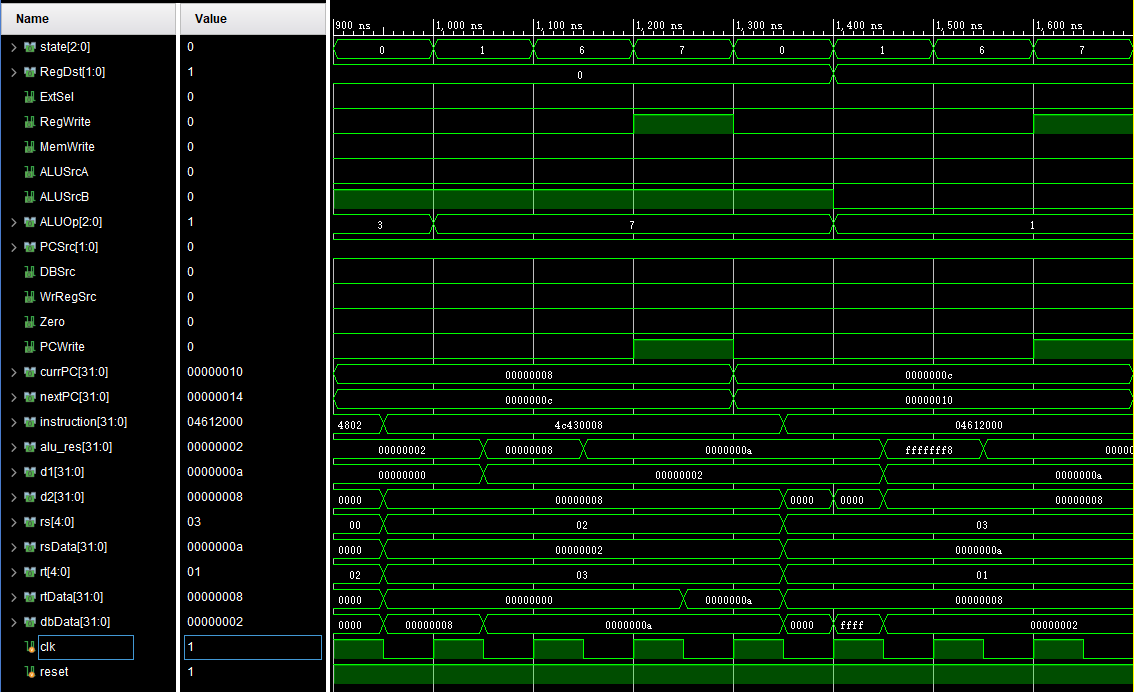
\includegraphics[width=0.9\linewidth]{fig/FullIns/Ins2.PNG}
\caption{波形图2}
\label{fig:wave_2}
\end{figure}
    \item \verb'0x10  and $5,$4,$2'\\
    WB(7)状态将结果$\mathrm{Reg}[4]\&\mathrm{Reg}[2]=2\&2=2$写入Reg[5]
    \item \verb'0x14  sll $5,$5,2'\\
    WB(7)状态将结果$\mathrm{Reg}[5]<<2=2<<2=8$写入Reg[5]
\begin{figure}[H]
\centering
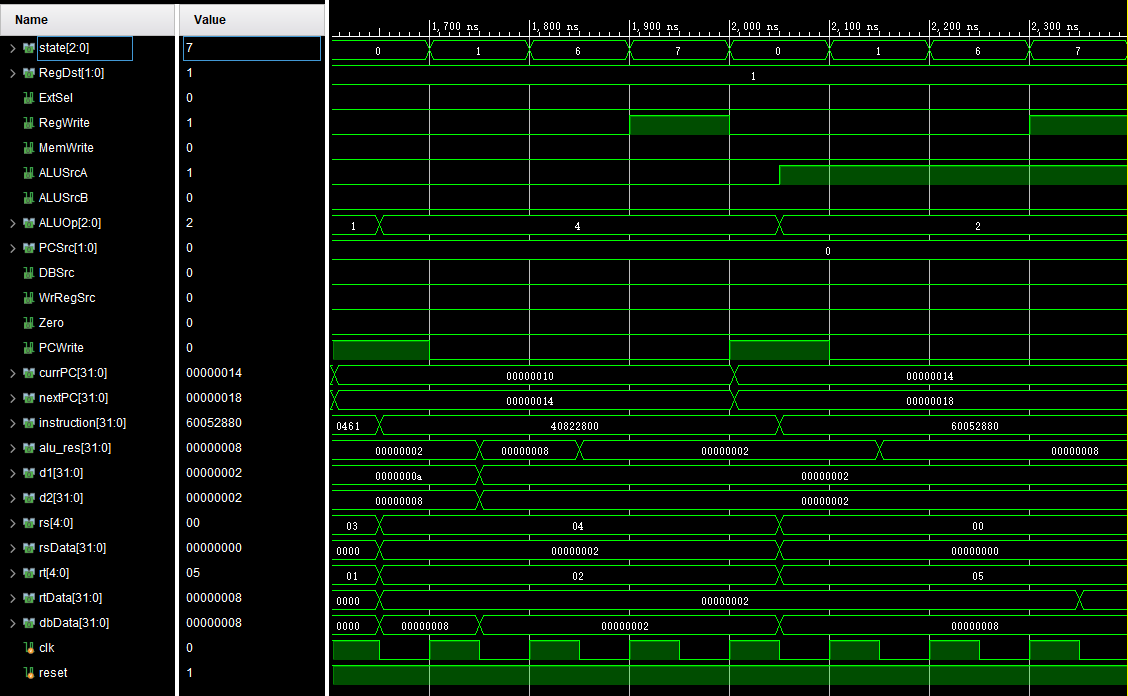
\includegraphics[width=0.9\linewidth]{fig/FullIns/Ins3.PNG}
\caption{波形图3}
\label{fig:wave_3}
\end{figure}
    \item \verb'0x18  beq $5,$1,-2'\\
    EXE(5)状态ALU结果为$\mathrm{Reg}[5]-\mathrm{Reg}[1]=8-8=0==0$,跳转回\verb'0x14'
    \item \verb'0x14  sll $5,$5,2'\\
    WB(7)状态将结果$\mathrm{Reg}[5]<<2=8<<2=32=(20)_{16}$写入Reg[5]
\begin{figure}[H]
\centering
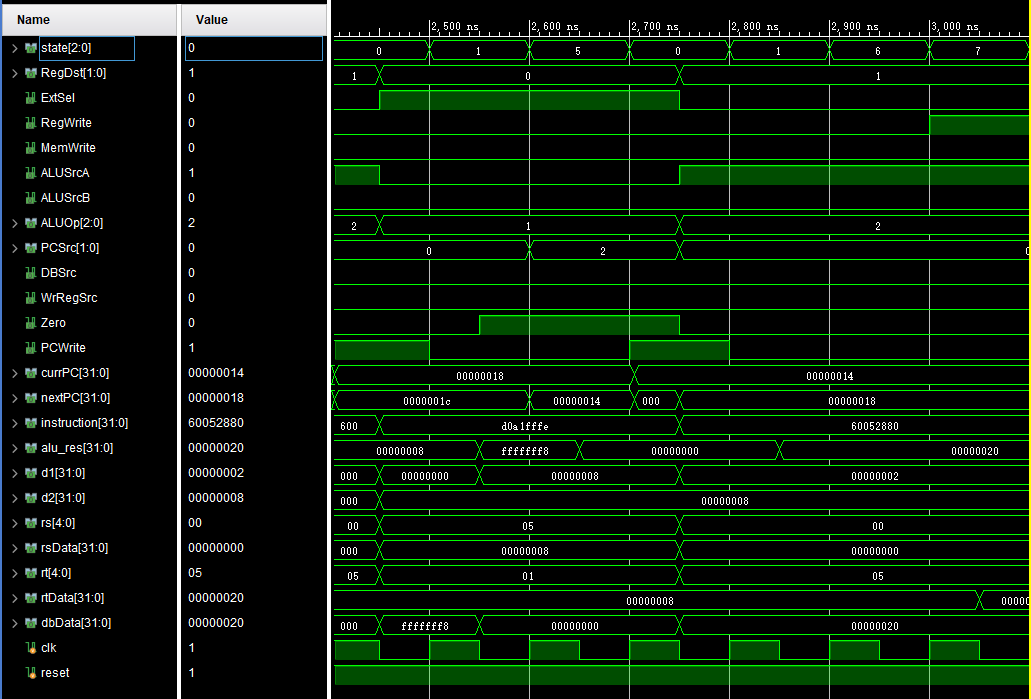
\includegraphics[width=0.9\linewidth]{fig/FullIns/Ins4.PNG}
\caption{波形图4}
\label{fig:wave_4}
\end{figure}
    \item \verb'0x18  beq $5,$1,-2'\\
    EXE(5)状态ALU结果为$\mathrm{Reg}[5]-\mathrm{Reg}[1]=32-8=24=(18)_{16}\ne 0$,不跳转,执行下一指令
    \item \verb'0x1C  jal 0x0000050'\\
    调用子程序,IF(0)状态更新下一PC值为\verb'0x50';ID(1)状态RegDst为2,对Reg[31]写入原来的PC+4,即\verb'0x20',故图中ALU在ID(1)状态的后半周期值回改变,因为RegFile写入了新的值
\begin{figure}[H]
\centering
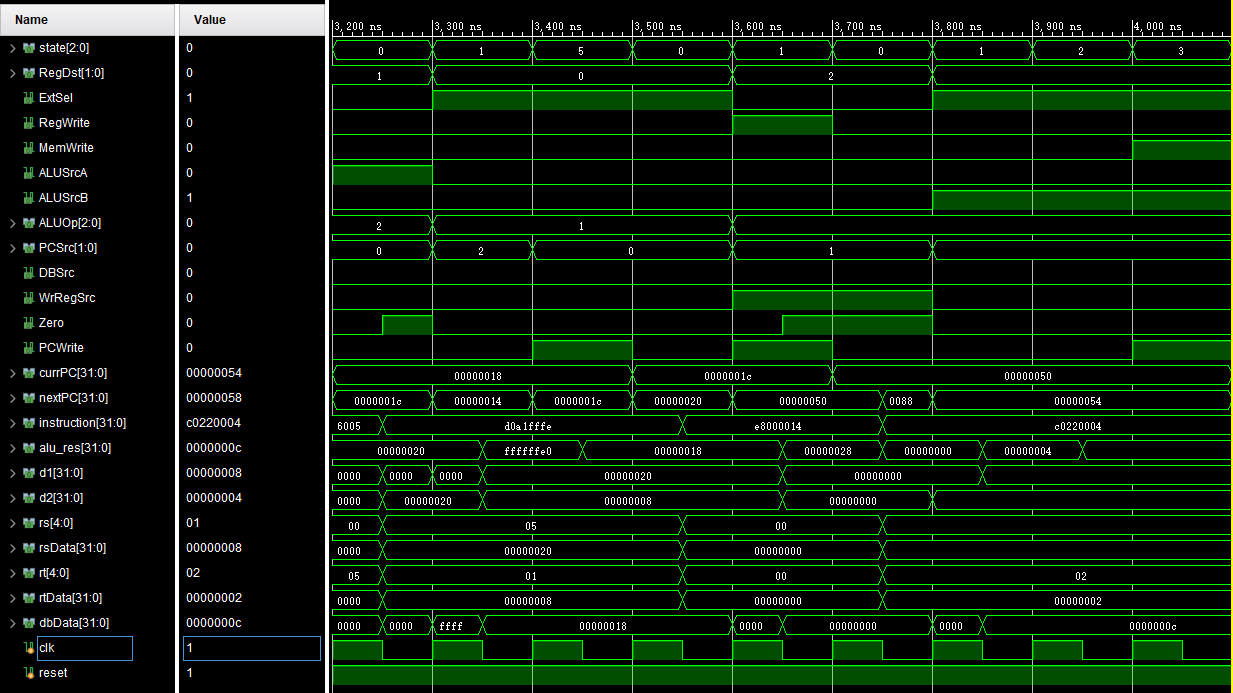
\includegraphics[width=0.8\linewidth]{fig/FullIns/Ins5.PNG}
\caption{波形图5}
\label{fig:wave_5}
\end{figure}
    \item \verb'0x50  sw $2,4($1)'\\
    将Reg[2]=2存入$\text{Mem}[\text{Reg}[1]+4]=\text{Reg}[12]=\text{Mem}[(C)_{16}]$
    \item \verb'0x54  lw $13,4($1)'\\
    将$\text{Mem}[12]=2$取出,在WB(4)状态存入Reg[13]
\begin{figure}[H]
\centering
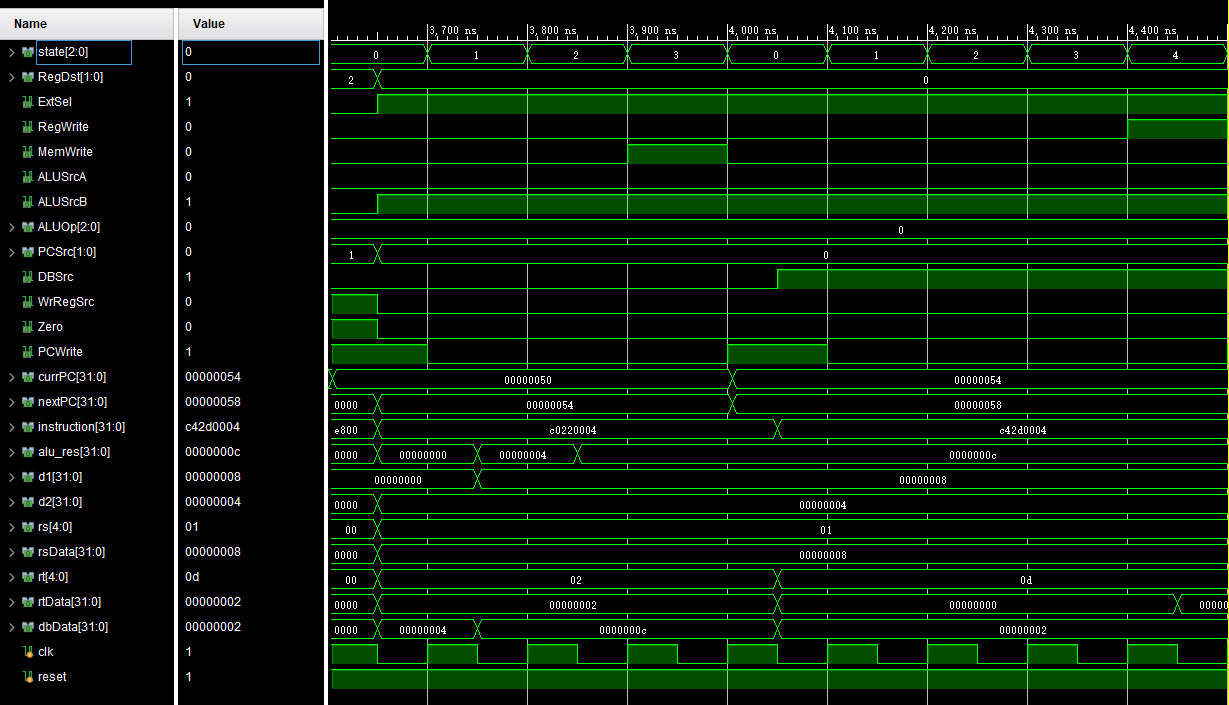
\includegraphics[width=0.9\linewidth]{fig/FullIns/Ins6.PNG}
\caption{波形图6}
\label{fig:wave_6}
\end{figure}
    \item \verb'0x58  jr $31'\\
    IF(0)状态译码后即可取出Reg[31]=\verb'0x20',进而更新下一PC值为\verb'0x20'
    \item \verb'0x20  slt $8,$13,$1'\\
    在EXE(6)阶段算得$\mathrm{Reg}[13]<\mathrm{Reg}[1]=2<8=1$,在WB(7)存入Reg[8]
\begin{figure}[H]
\centering
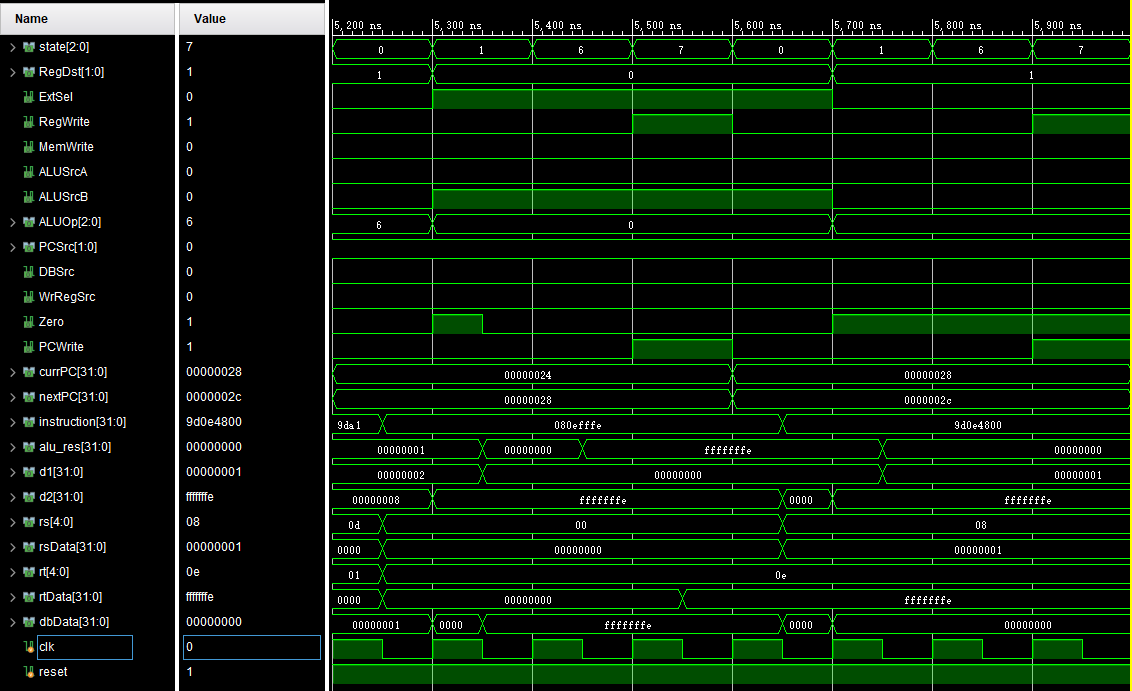
\includegraphics[width=0.9\linewidth]{fig/FullIns/Ins7.PNG}
\caption{波形图7}
\label{fig:wave_7}
\end{figure}
    \item \verb'0x24  addiu $14,$0,-2'\\
    在EXE(6)阶段算得Reg[0]+(-2)=\verb'0xFFFFFFFE',并在WB(7)存入Reg[14]
    \item \verb'0x28  slt $9,$8,$14'\\
    在EXE(6)阶段算得Reg[8]<Reg[14]=1<-2=0,并在WB(7)存入Reg[9]
\begin{figure}[H]
\centering
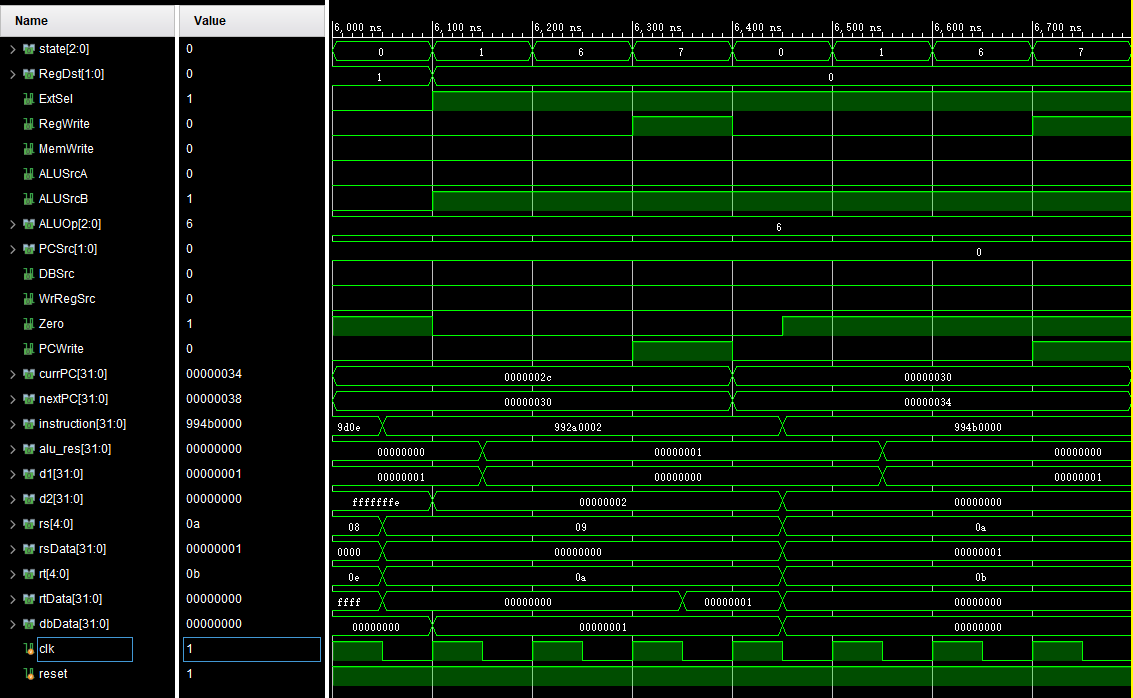
\includegraphics[width=0.9\linewidth]{fig/FullIns/Ins8.PNG}
\caption{波形图8}
\label{fig:wave_8}
\end{figure}
    \item \verb'0x2C  slti $10,$9,2'\\
    在EXE(6)阶段算得Reg[9]<2=0<2=1,并在WB(7)存入Reg[10]
    \item \verb'0x30  slti $11,$10,0'\\
    在EXE(6)阶段算得Reg[10]<=0=1<0=0,并在WB(7)存入Reg[11]
\begin{figure}[H]
\centering
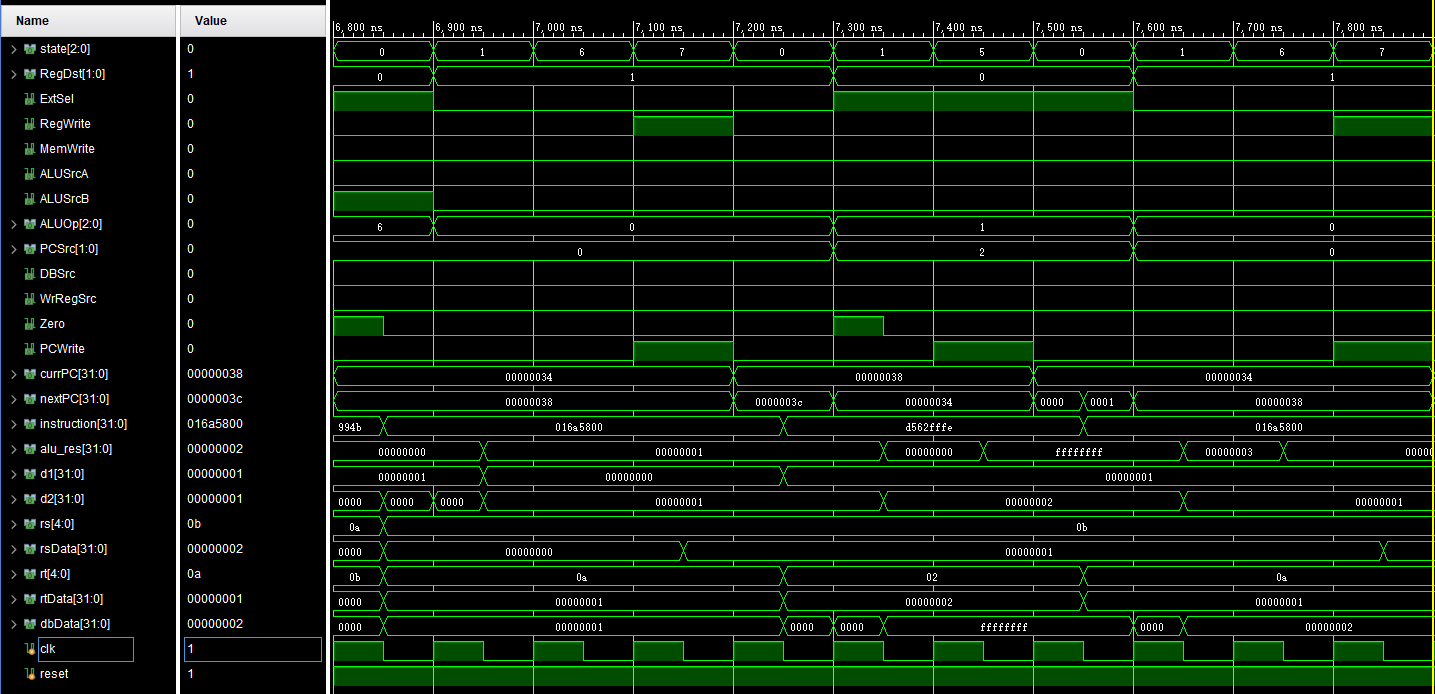
\includegraphics[width=0.9\linewidth]{fig/FullIns/Ins9.PNG}
\caption{波形图9}
\label{fig:wave_9}
\end{figure}
    \item \verb'0x34  add $11,$11,$10'\\
    在EXE(6)阶段算得Reg[11]+Reg[10]=0+1=1,并在WB(7)存入Reg[11]
    \item \verb'0x38  bne $11,$2,-2'\\
    在EXE(5)阶段算得Reg[11]-Reg[2]=1-2=-1=\verb'0xFFFFFFFF',不等于,跳转回\verb'0x34'
\begin{figure}[H]
\centering
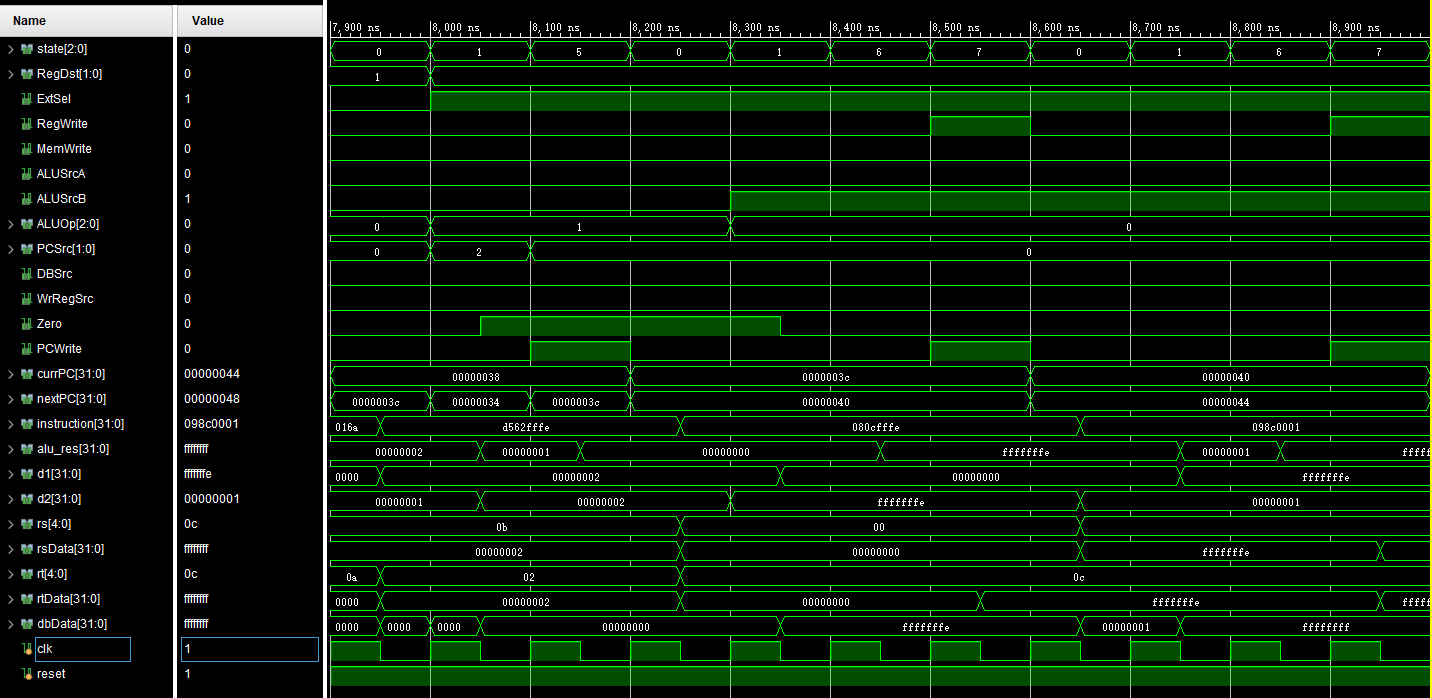
\includegraphics[width=0.9\linewidth]{fig/FullIns/Ins10.PNG}
\caption{波形图10}
\label{fig:wave_10}
\end{figure}
    \item \verb'0x34  add $11,$11,$10'\\
    在EXE(6)阶段算得Reg[11]+Reg[10]=1+1=2,并在WB(7)存入Reg[11]
    \item \verb'0x38  bne $11,$2,-2'\\
    在EXE(5)阶段算得Reg[11]-Reg[2]=2-2=0,相等,不跳转,执行下条指令
\begin{figure}[H]
\centering
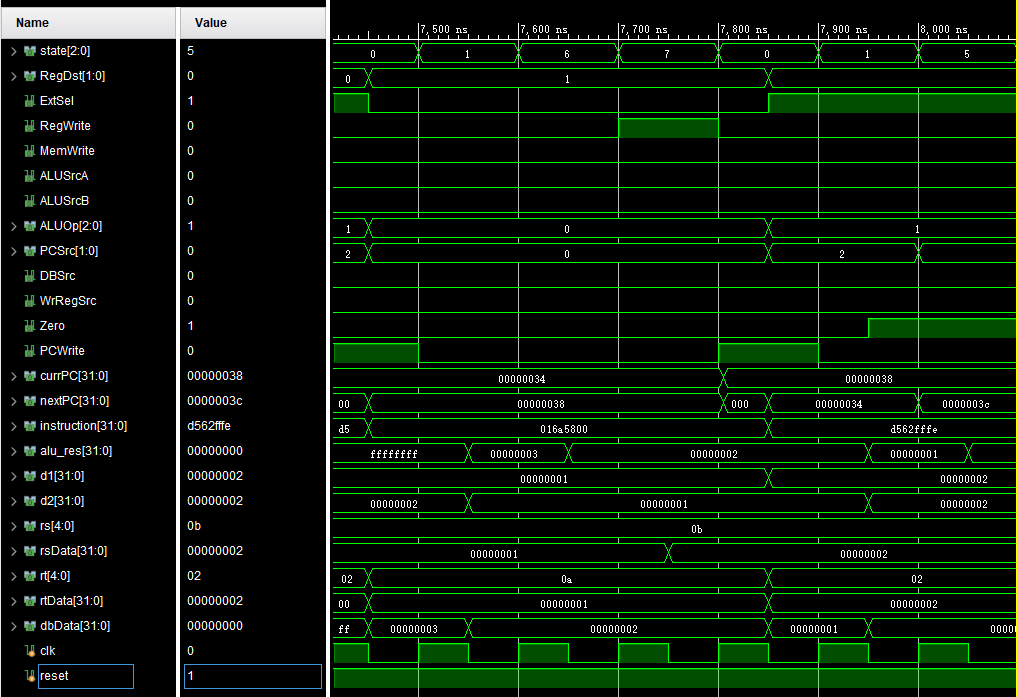
\includegraphics[width=0.9\linewidth]{fig/FullIns/Ins11.PNG}
\caption{波形图11}
\label{fig:wave_11}
\end{figure}
    \item \verb'0x3C  addiu $12,$0,-2'\\
    在EXE(6)阶段算得Reg[0]+(-2)=\verb'0xFFFFFFFE',并在WB(7)存入Reg[12]
    \item \verb'0x40  addiu $12,$12,1'\\
    在EXE(6)阶段算得Reg[12]+1=\verb'0xFFFFFFFF',并在WB(7)存入Reg[12]
\begin{figure}[H]
\centering
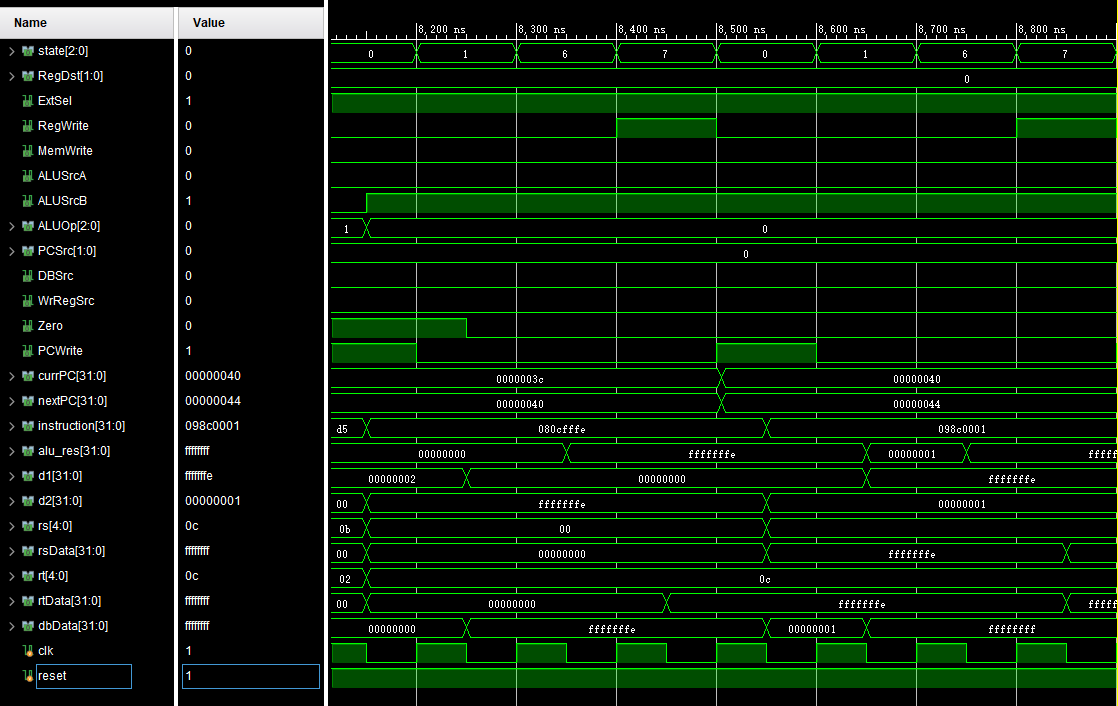
\includegraphics[width=0.9\linewidth]{fig/FullIns/Ins12.PNG}
\caption{波形图12}
\label{fig:wave_12}
\end{figure}
    \item \verb'0x44  bltz $12,-2'\\
    在EXE(5)阶段算得Reg[12]<0=-1<0=1,故跳转回\verb'0x40'
    \item \verb'0x40  addiu $12,$12,1'\\
    在EXE(6)阶段算得Reg[12]+1=0,并在WB(7)存入Reg[12]
\begin{figure}[H]
\centering
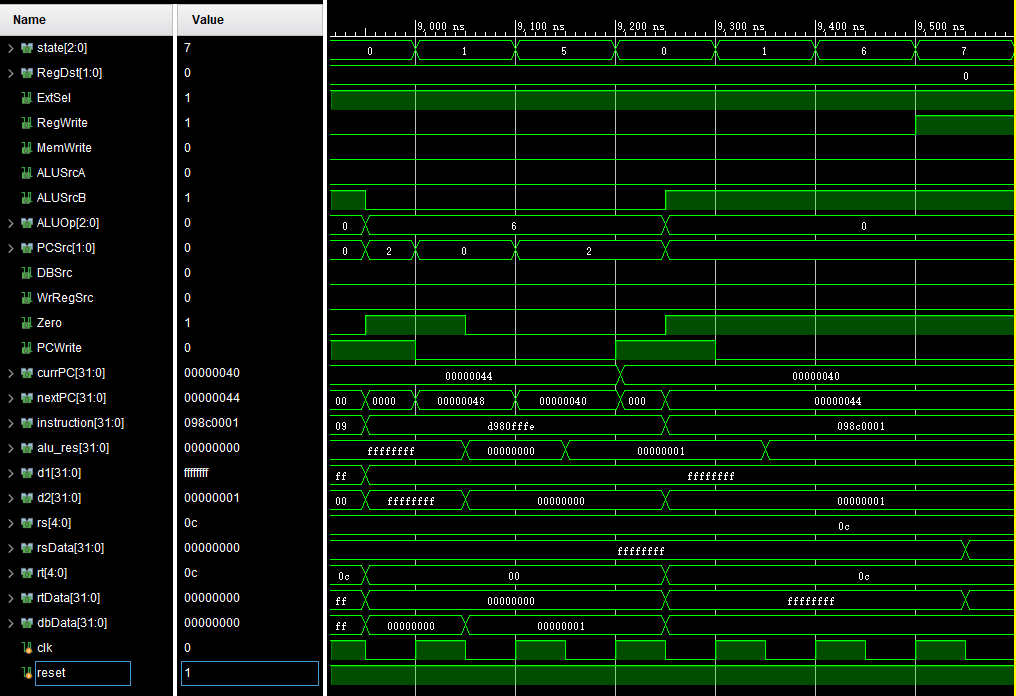
\includegraphics[width=0.9\linewidth]{fig/FullIns/Ins13.PNG}
\caption{波形图13}
\label{fig:wave_13}
\end{figure}
    \item \verb'0x44  bltz $12,-2'\\
    在EXE(5)阶段算得Reg[12]<0=0<0=0,故不跳转,继续执行下一指令
    \item \verb'0x48  andi $12,$2,2'\\
    在EXE(6)阶段算得Reg[2]\&2=2\&2=2,并在WB(7)存入Reg[12]
\begin{figure}[H]
\centering
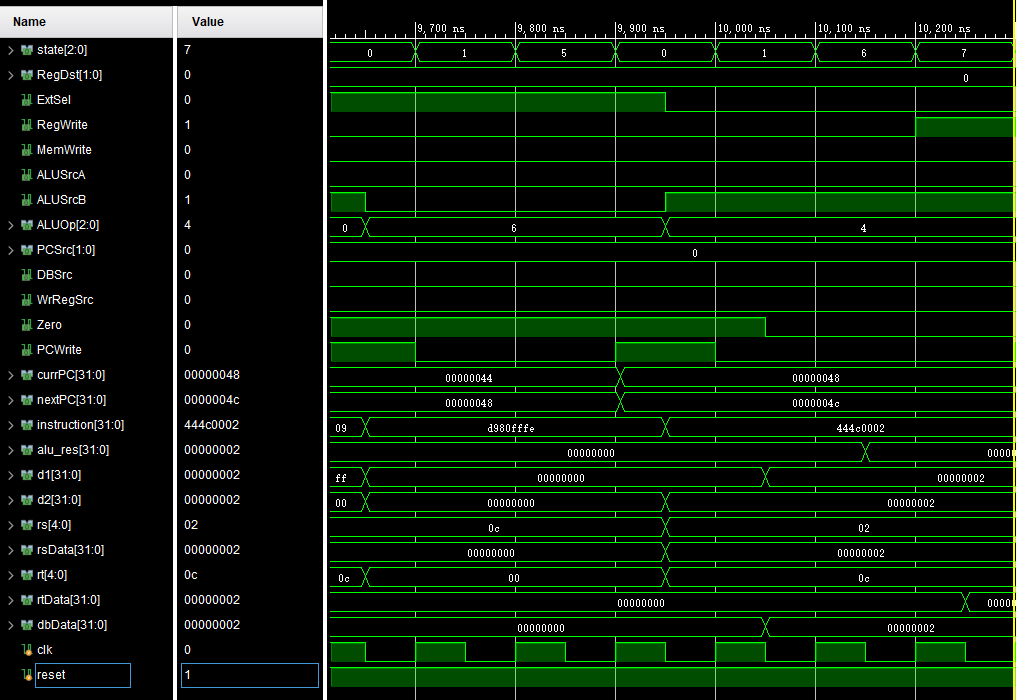
\includegraphics[width=0.9\linewidth]{fig/FullIns/Ins14.PNG}
\caption{波形图14}
\label{fig:wave_14}
\end{figure}
    \item \verb'0x50  j 0x000005C'\\
    在IF(0)后半阶段写入指令到IR,译码得出其为跳转指令,更新下一PC值为\verb'0x5C'
    \item \verb'halt'\\
    在ID(1)阶段求得指令为停机,不再更新PC
\begin{figure}[H]
\centering
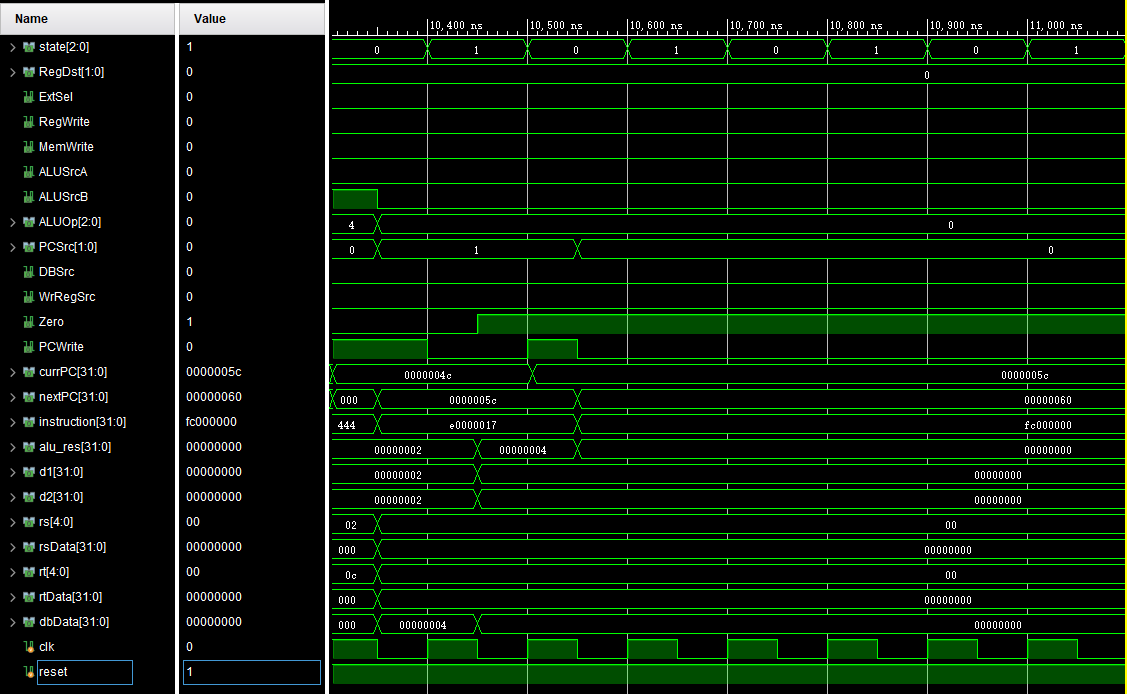
\includegraphics[width=0.9\linewidth]{fig/FullIns/Ins15.PNG}
\caption{波形图15}
\label{fig:wave_15}
\end{figure}
\end{enumerate}
% !TEX root = main.tex

\subsection{上板}
\qquad 几条代表性指令的Basys3板结果如下,其他指令结果见具体实现。从左到右从上到下四幅图依次是:当前/下条PC、rs寄存器地址/值、rt寄存器地址/值、ALU结果输出/DB总线数据。\textcolor{red}{注意这里显示的都是最后一个状态的值。又由于这些信号都采用wire类型,故写入寄存器后可能导致alu\_res的相应改变。}但可以看见上板结果与前面仿真分析的结果相同,这成功证明了程序的正确性。
\begin{enumerate}
    \item 0x00: \verb'addiu $1, $0, 8'
    \begin{figure}[H]
    \centering
    \begin{tabular}{cc}
    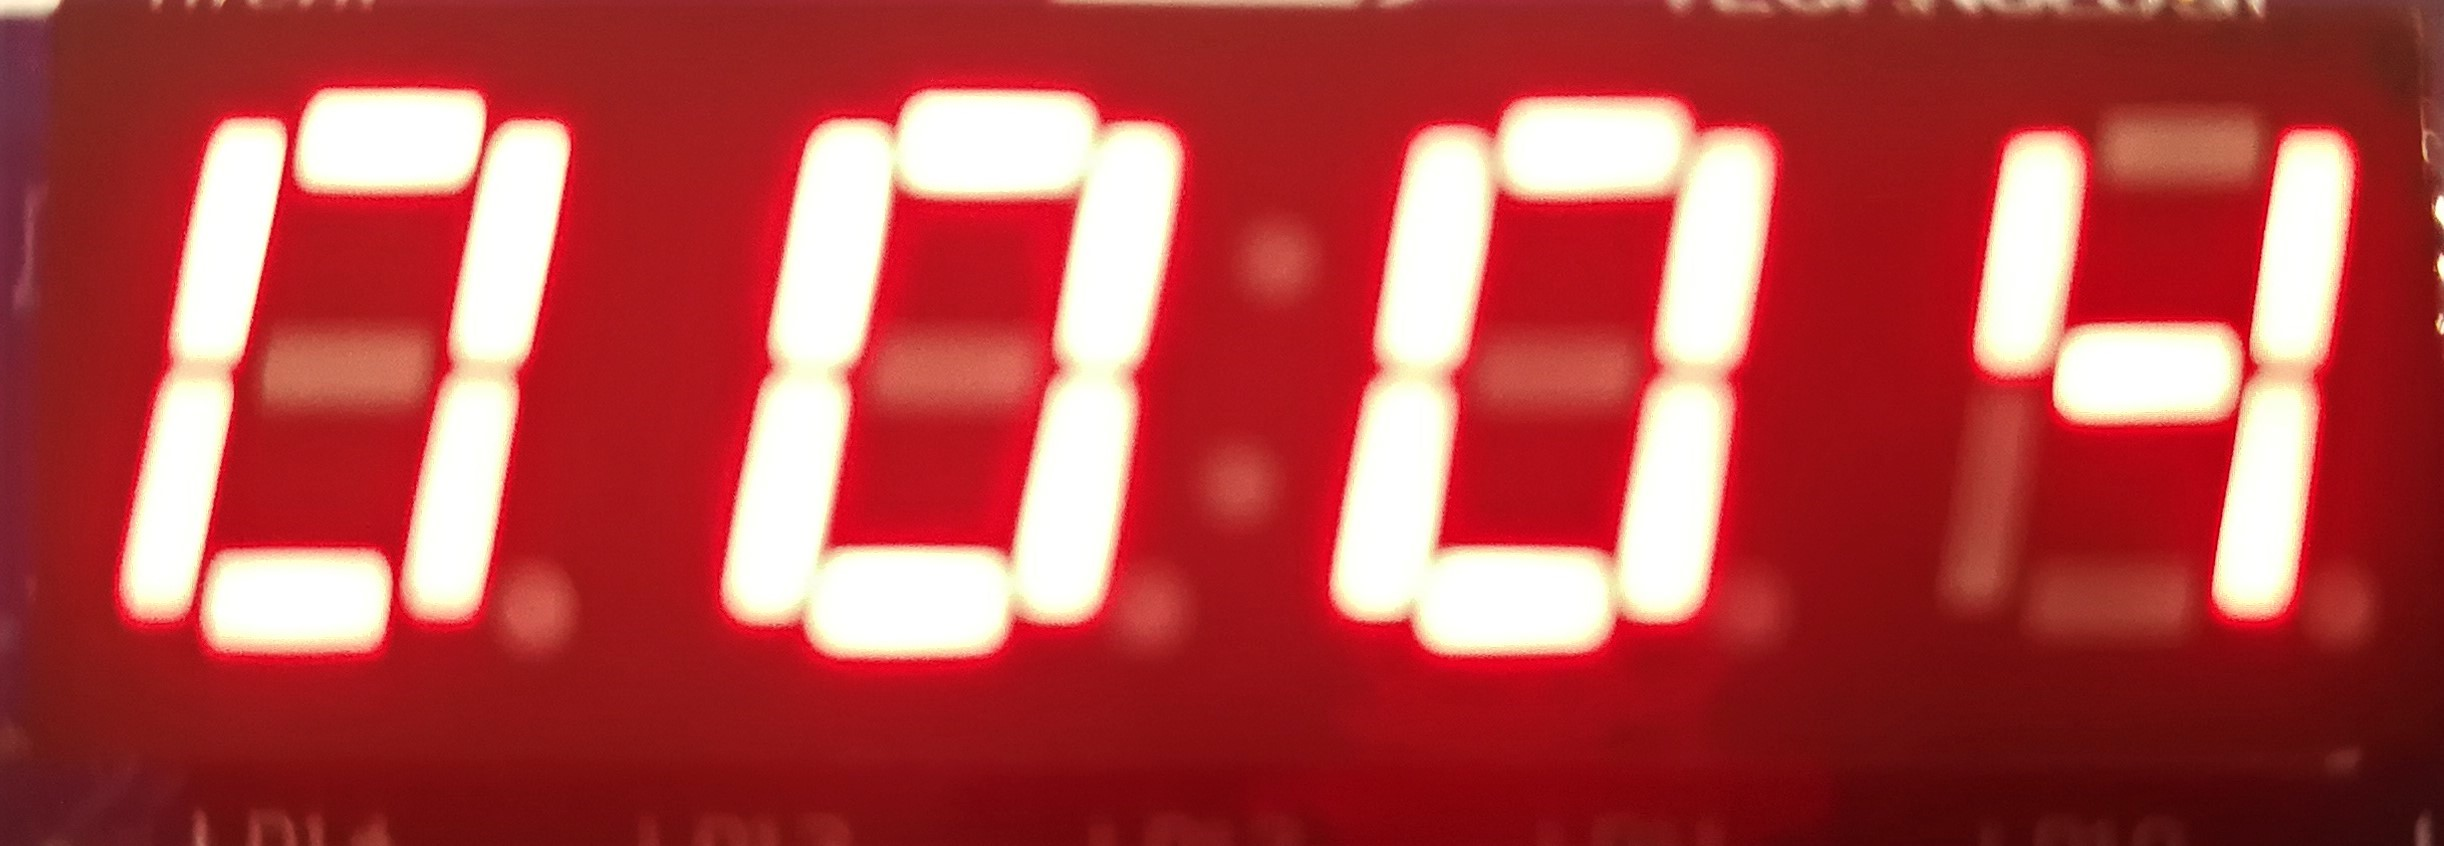
\includegraphics[width=0.3\linewidth]{fig/Implementation/0x00_00.jpg}&
    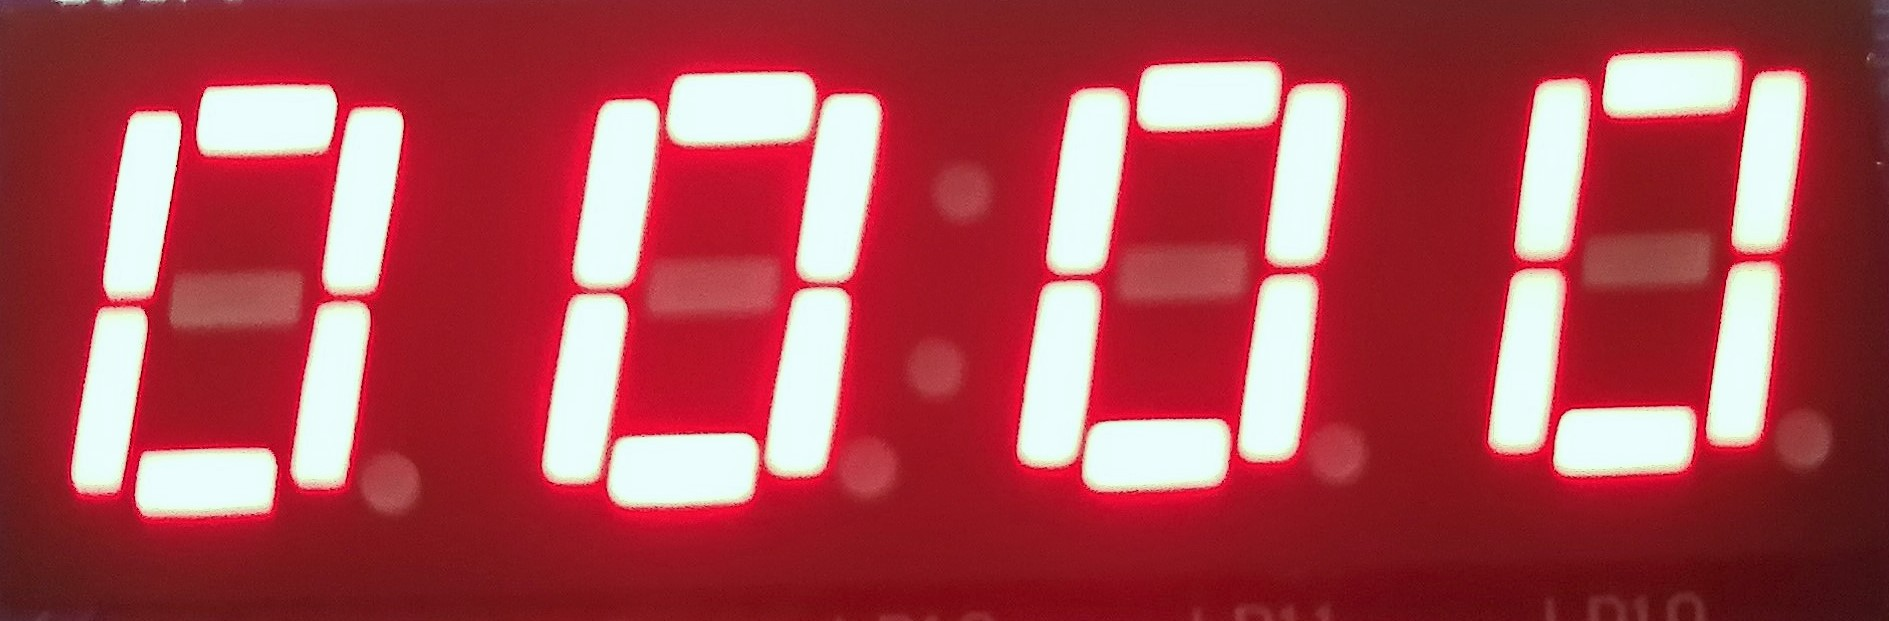
\includegraphics[width=0.3\linewidth]{fig/Implementation/0x00_01.jpg}\\
    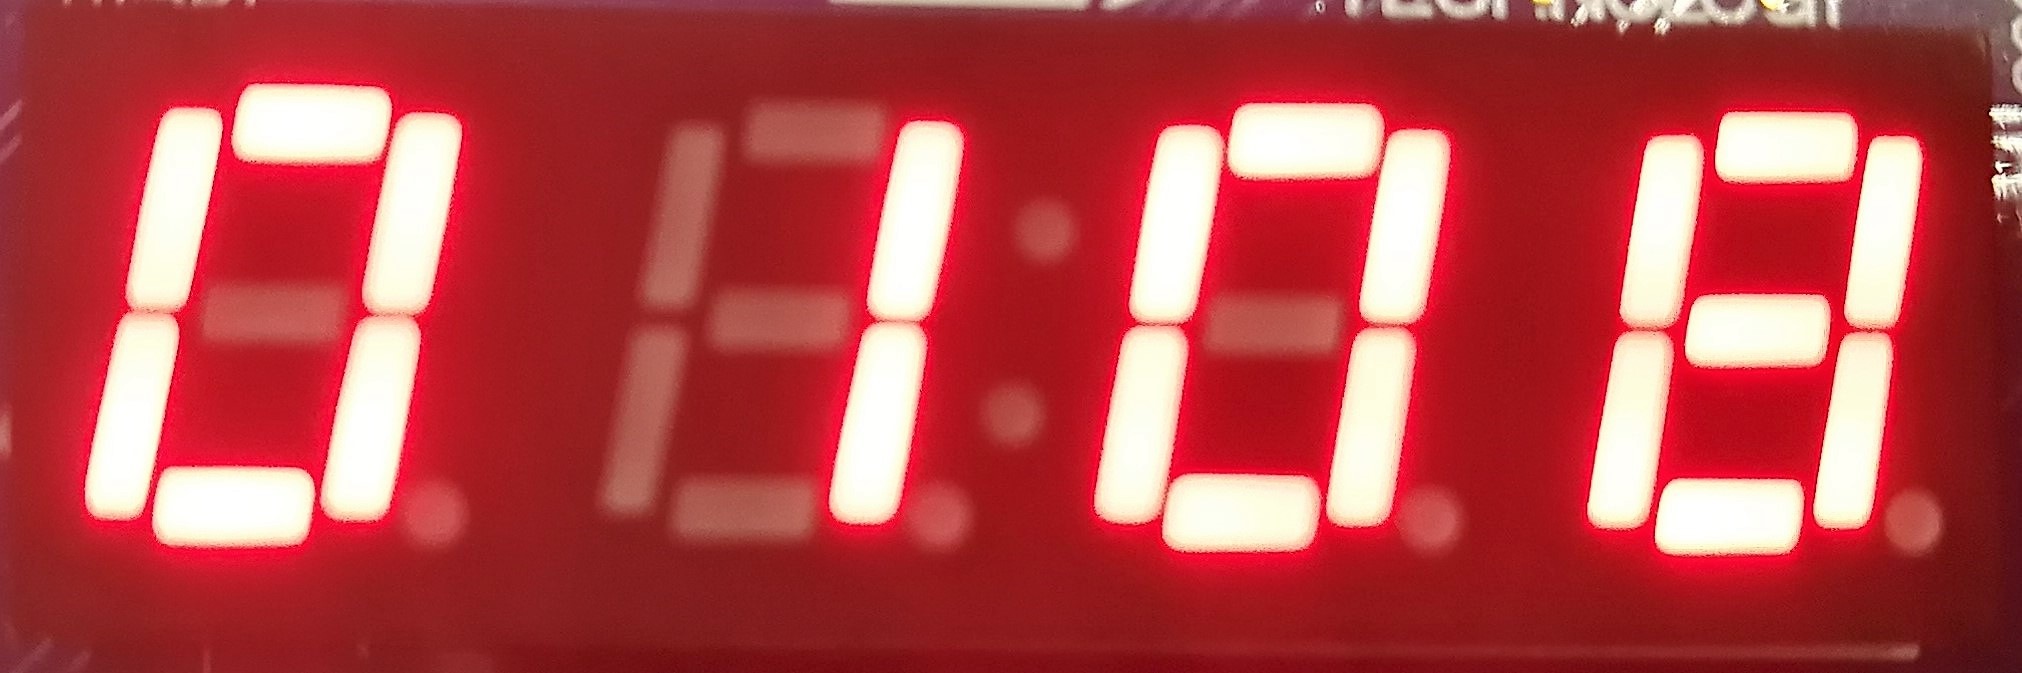
\includegraphics[width=0.3\linewidth]{fig/Implementation/0x00_10.jpg}&
    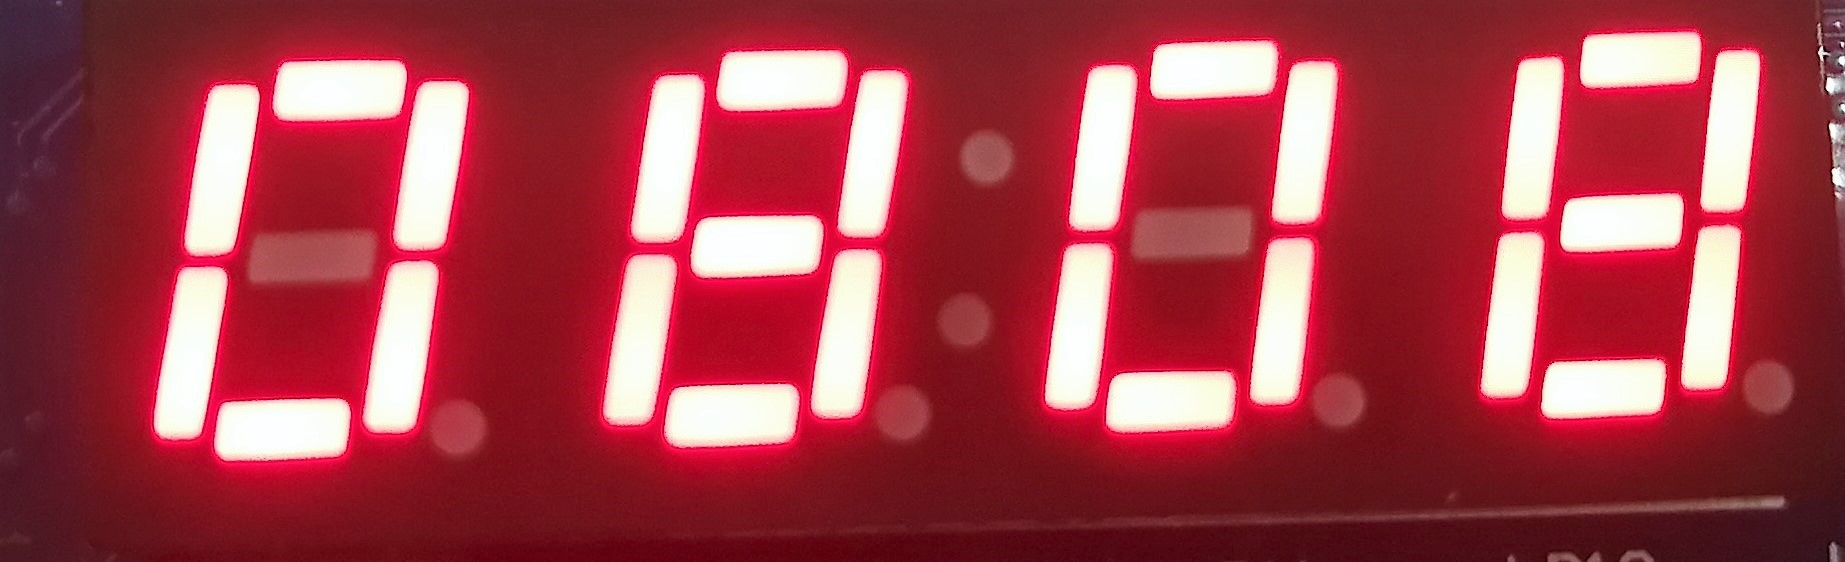
\includegraphics[width=0.3\linewidth]{fig/Implementation/0x00_11.jpg}
    \end{tabular}
    \caption{0x00结果}
    \end{figure}
    \item 0x14: \verb'sll $5, $5, 2'
    \begin{figure}[H]
    \centering
    \begin{tabular}{cc}
    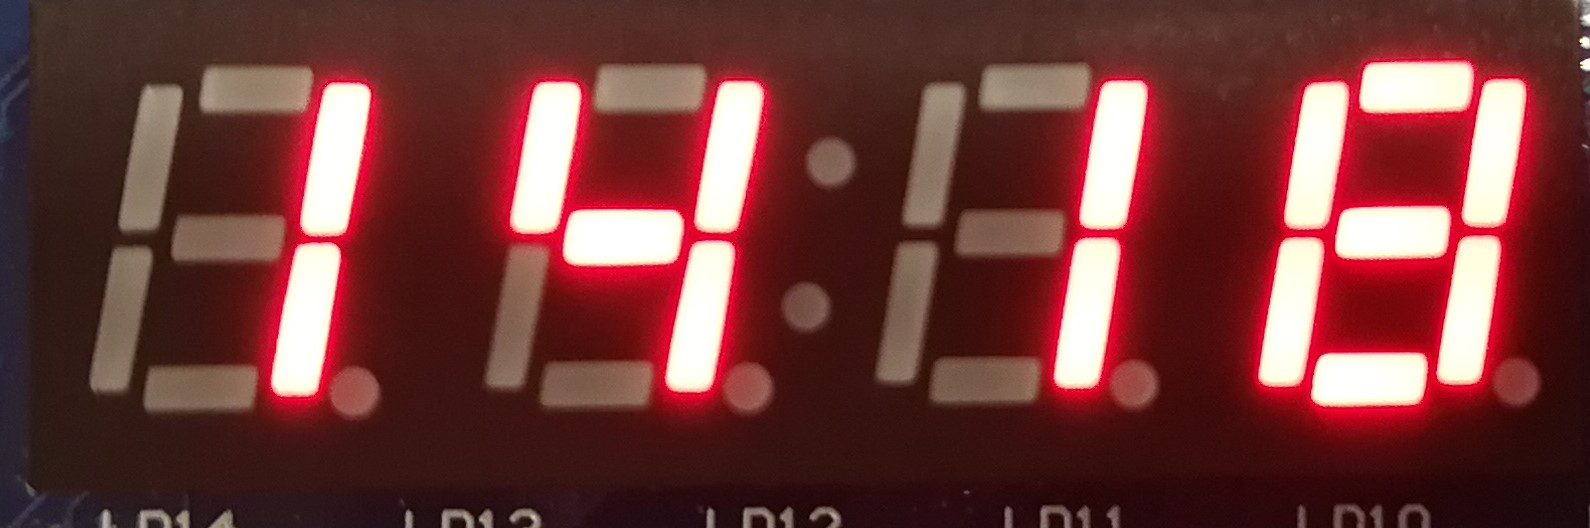
\includegraphics[width=0.3\linewidth]{fig/Implementation/0x14_00.jpg}&
    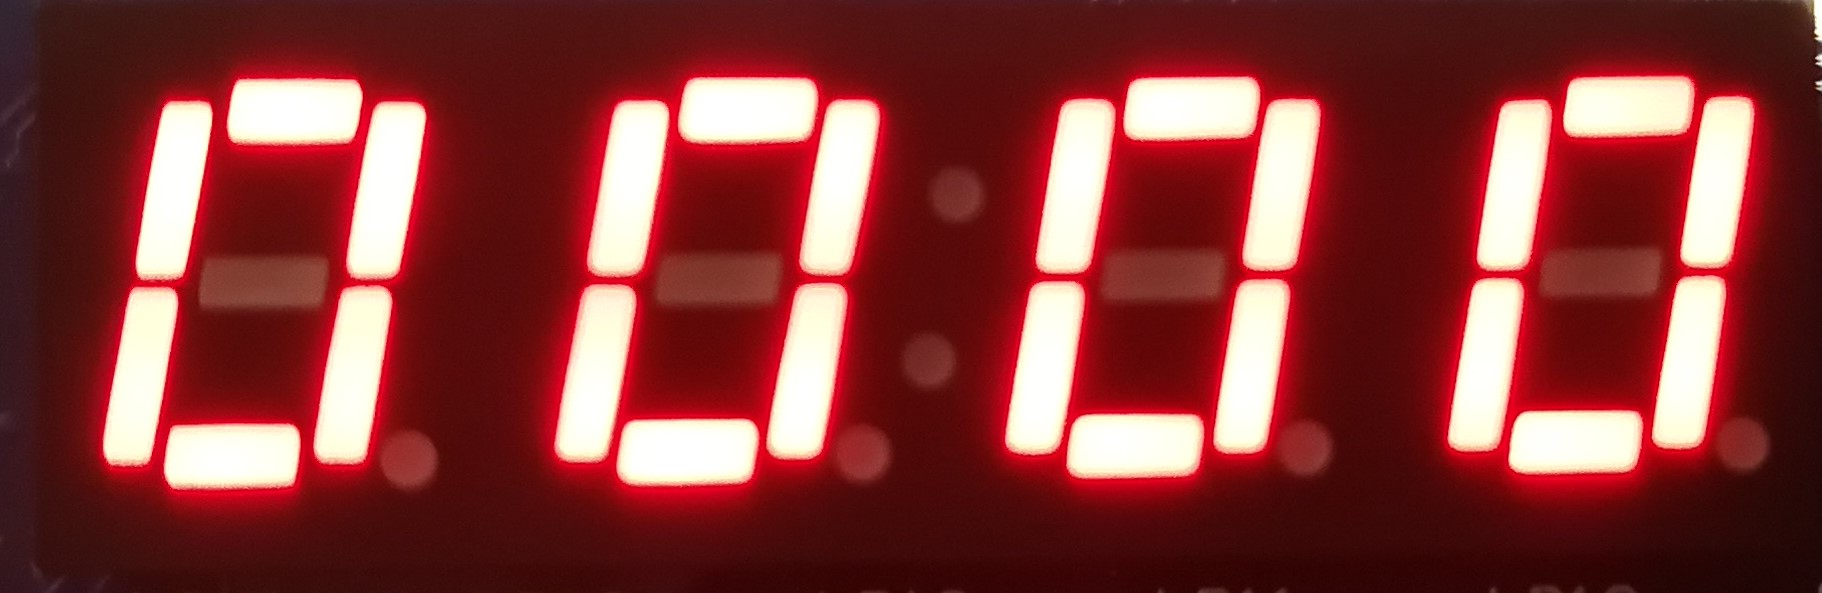
\includegraphics[width=0.3\linewidth]{fig/Implementation/0x14_01.jpg}\\
    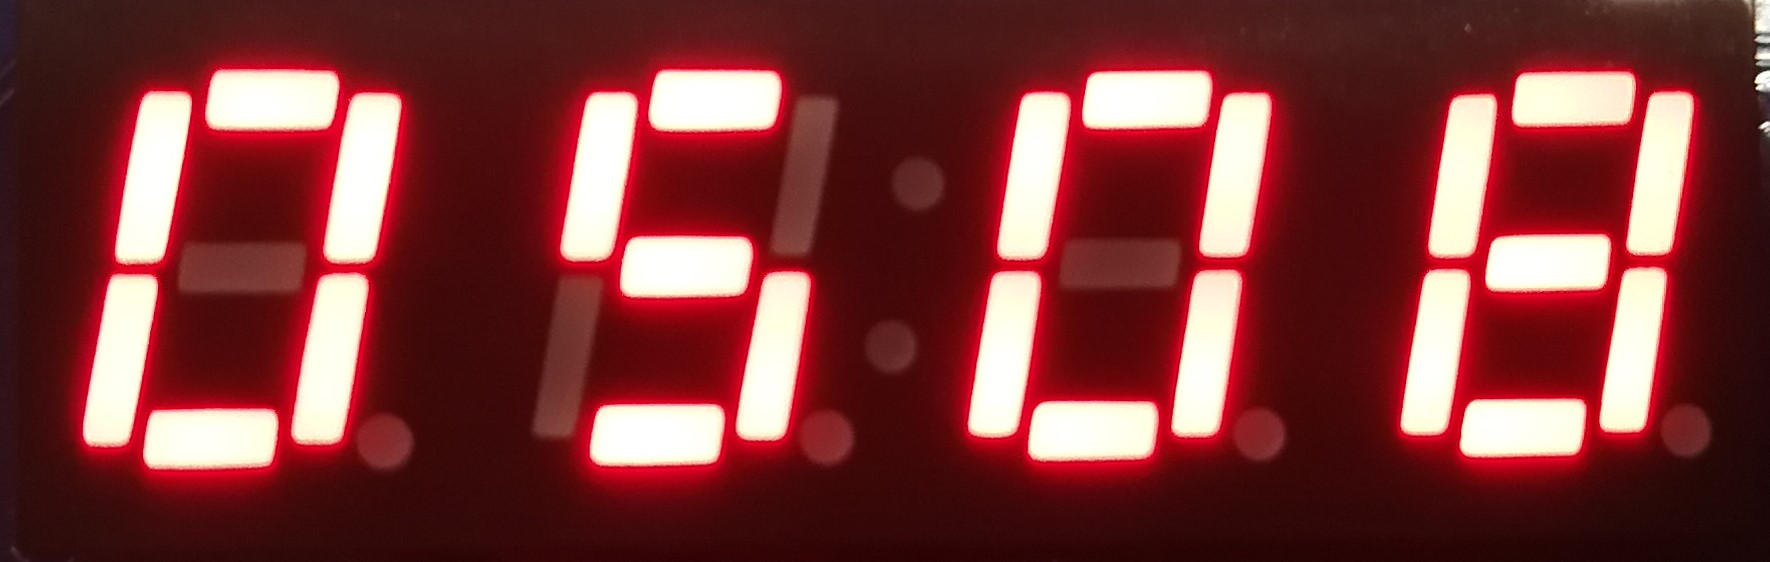
\includegraphics[width=0.3\linewidth]{fig/Implementation/0x14_10.jpg}&
    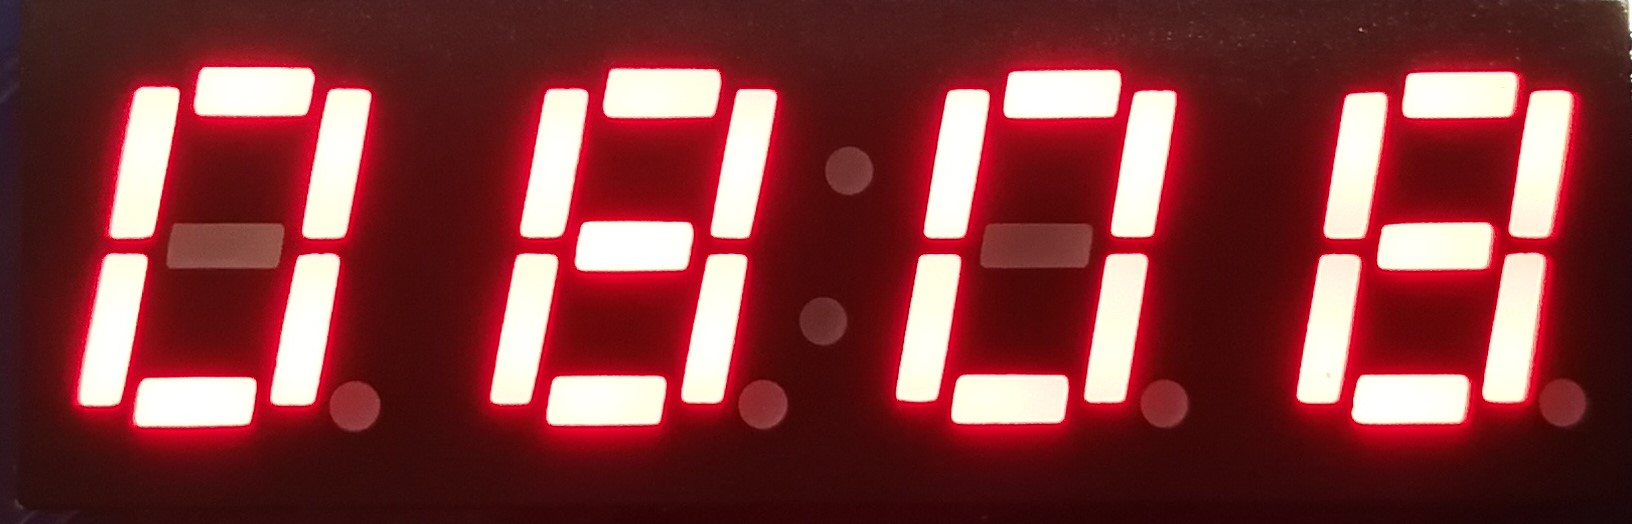
\includegraphics[width=0.3\linewidth]{fig/Implementation/0x14_11.jpg}
    \end{tabular}
    \caption{0x14结果}
    \end{figure}
    \item 0x18: \verb'beq $5, $1, -2'
    \begin{figure}[H]
    \centering
    \begin{tabular}{cc}
    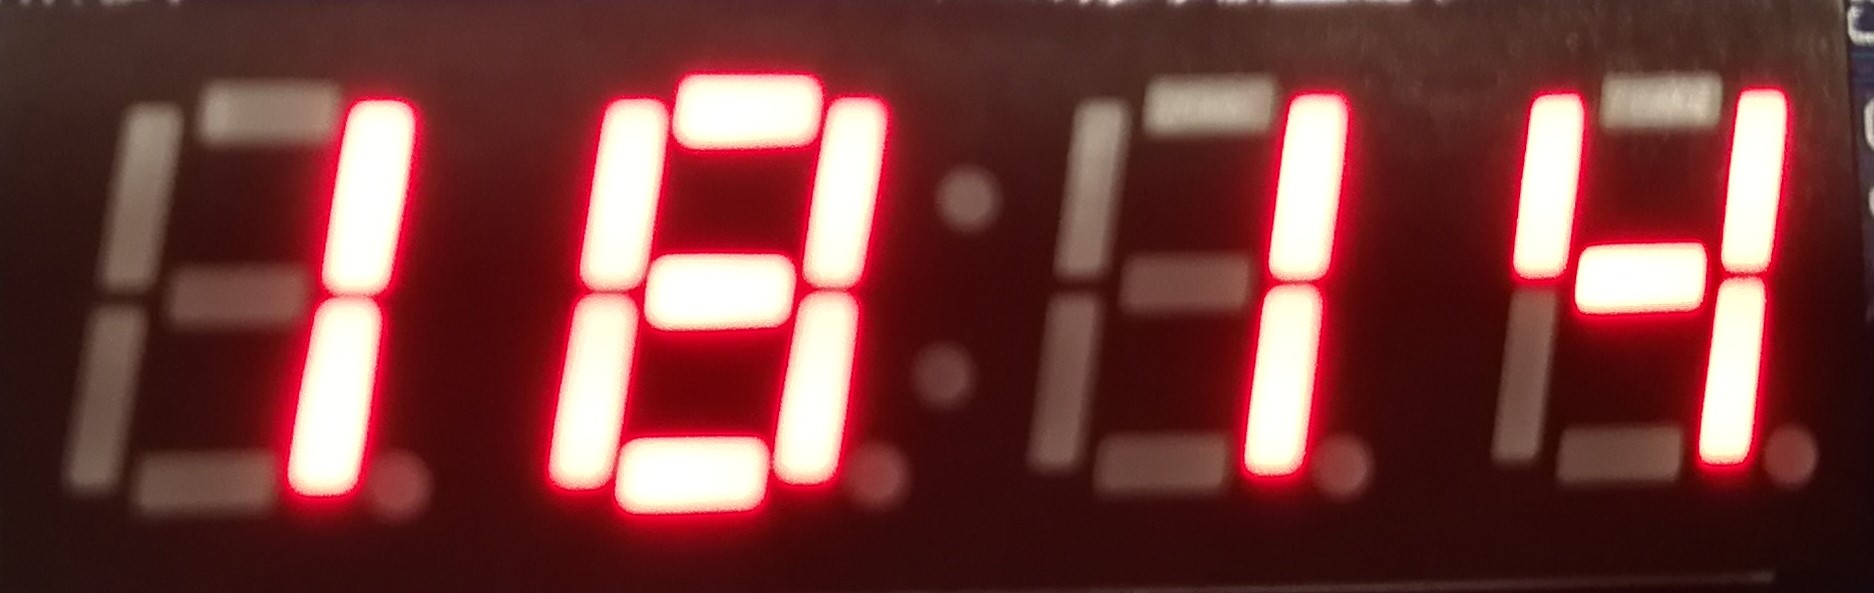
\includegraphics[width=0.3\linewidth]{fig/Implementation/0x18_00.jpg}&
    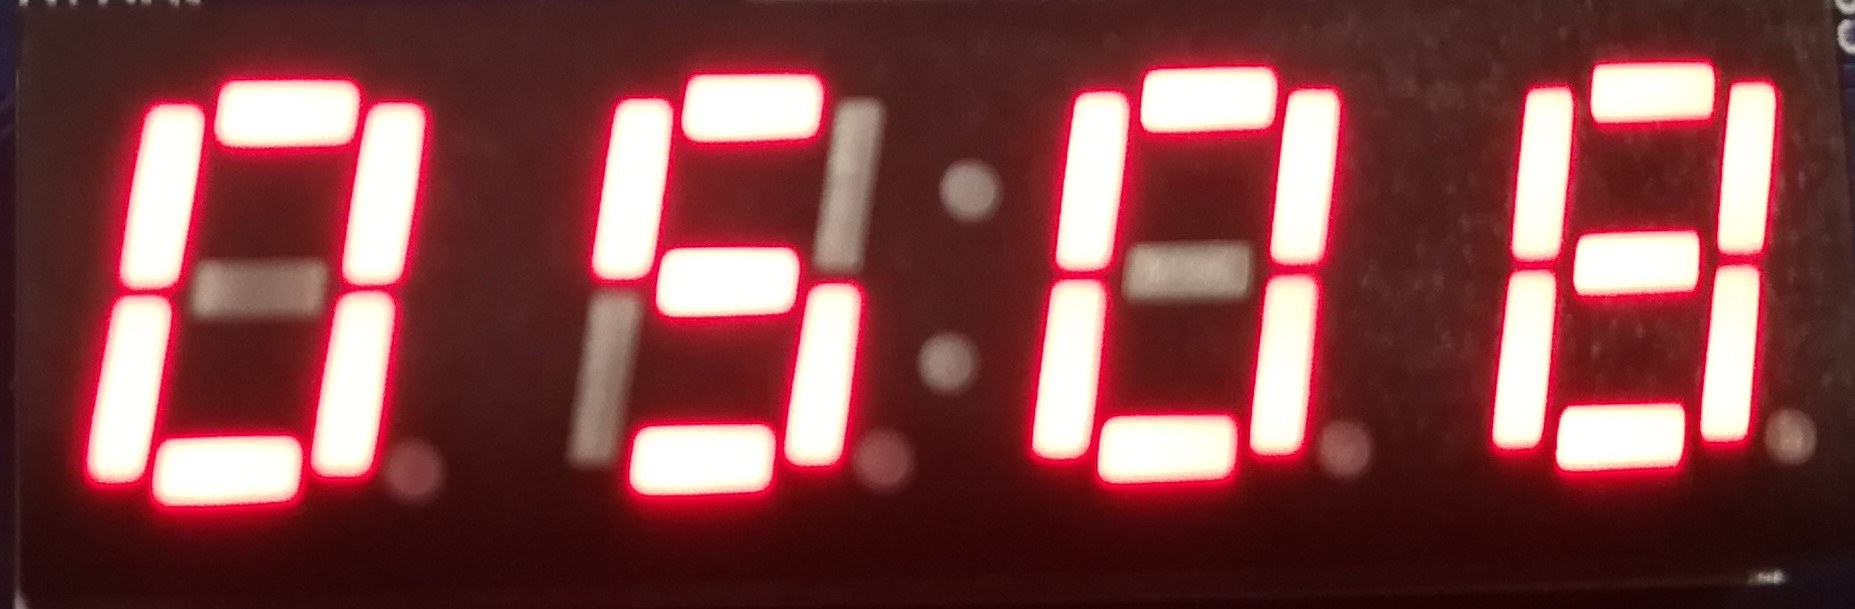
\includegraphics[width=0.3\linewidth]{fig/Implementation/0x18_01.jpg}\\
    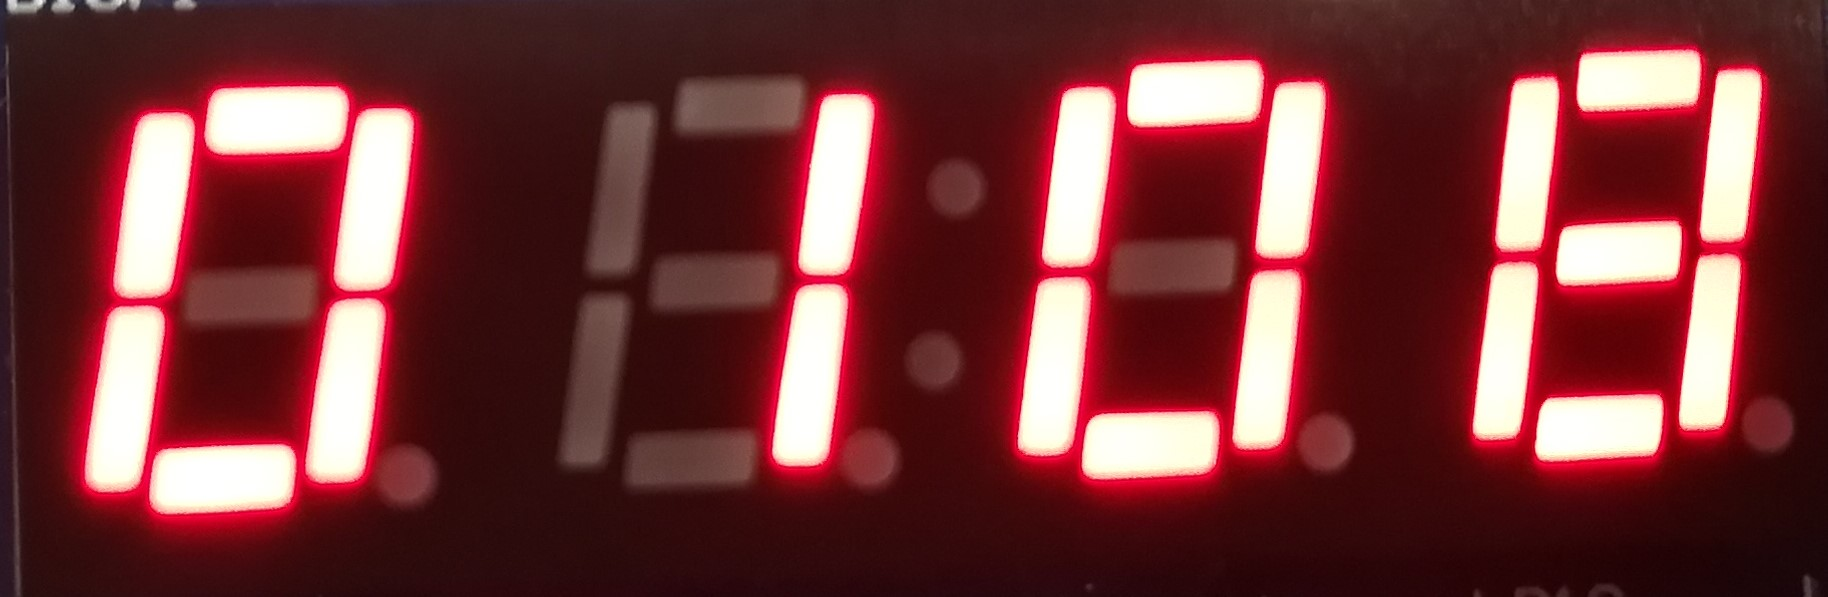
\includegraphics[width=0.3\linewidth]{fig/Implementation/0x18_10.jpg}&
    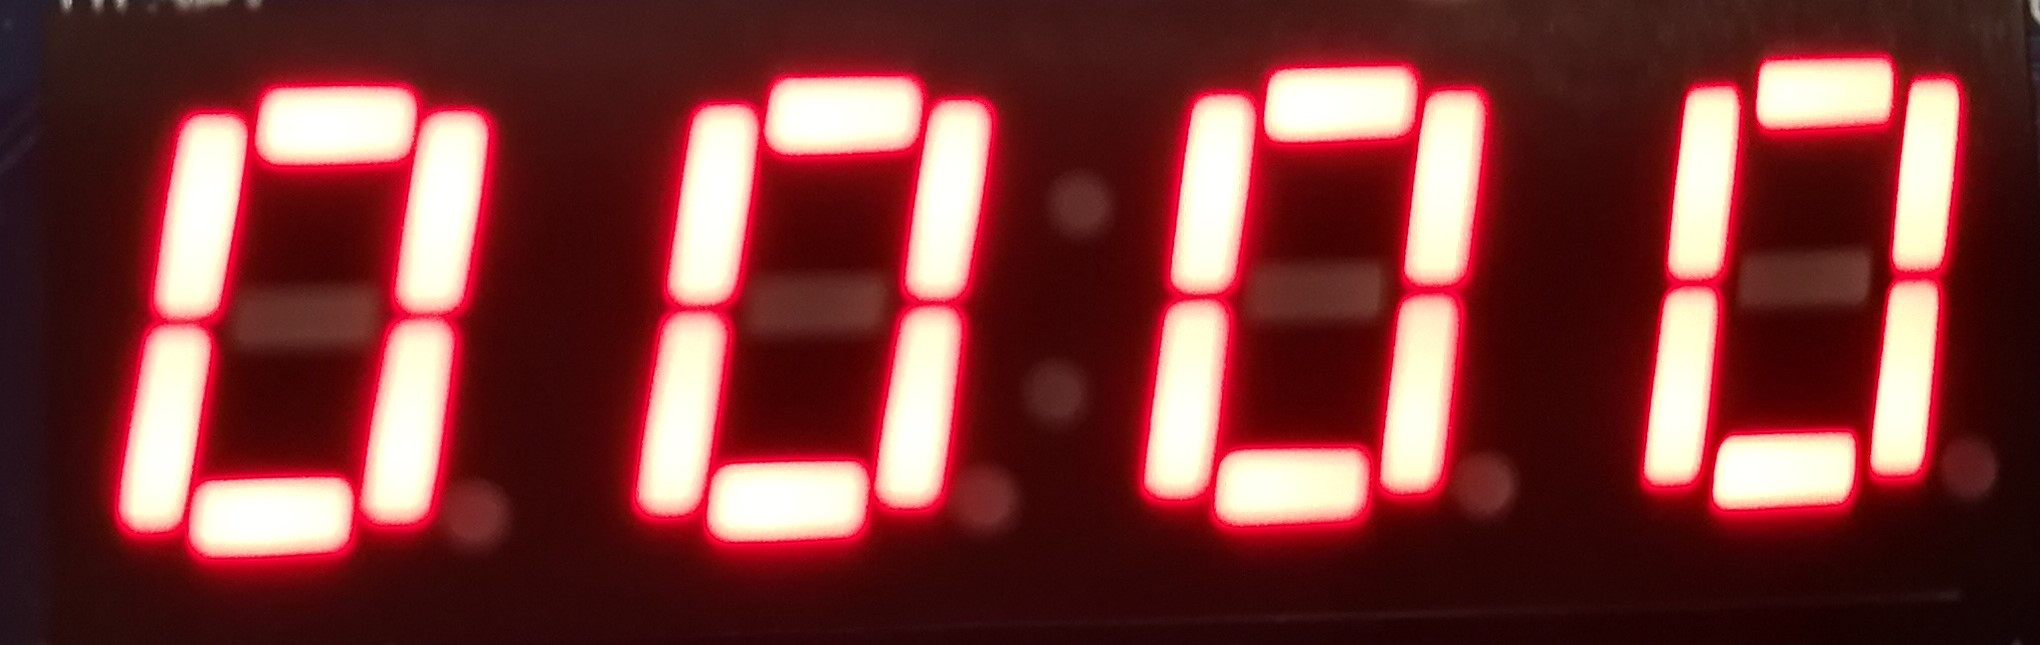
\includegraphics[width=0.3\linewidth]{fig/Implementation/0x18_11.jpg}
    \end{tabular}
    \caption{0x18结果}
    \end{figure}
    \item 0x1C: \verb'jal 0x0000050'
    \begin{figure}[H]
    \centering
    \begin{tabular}{cc}
    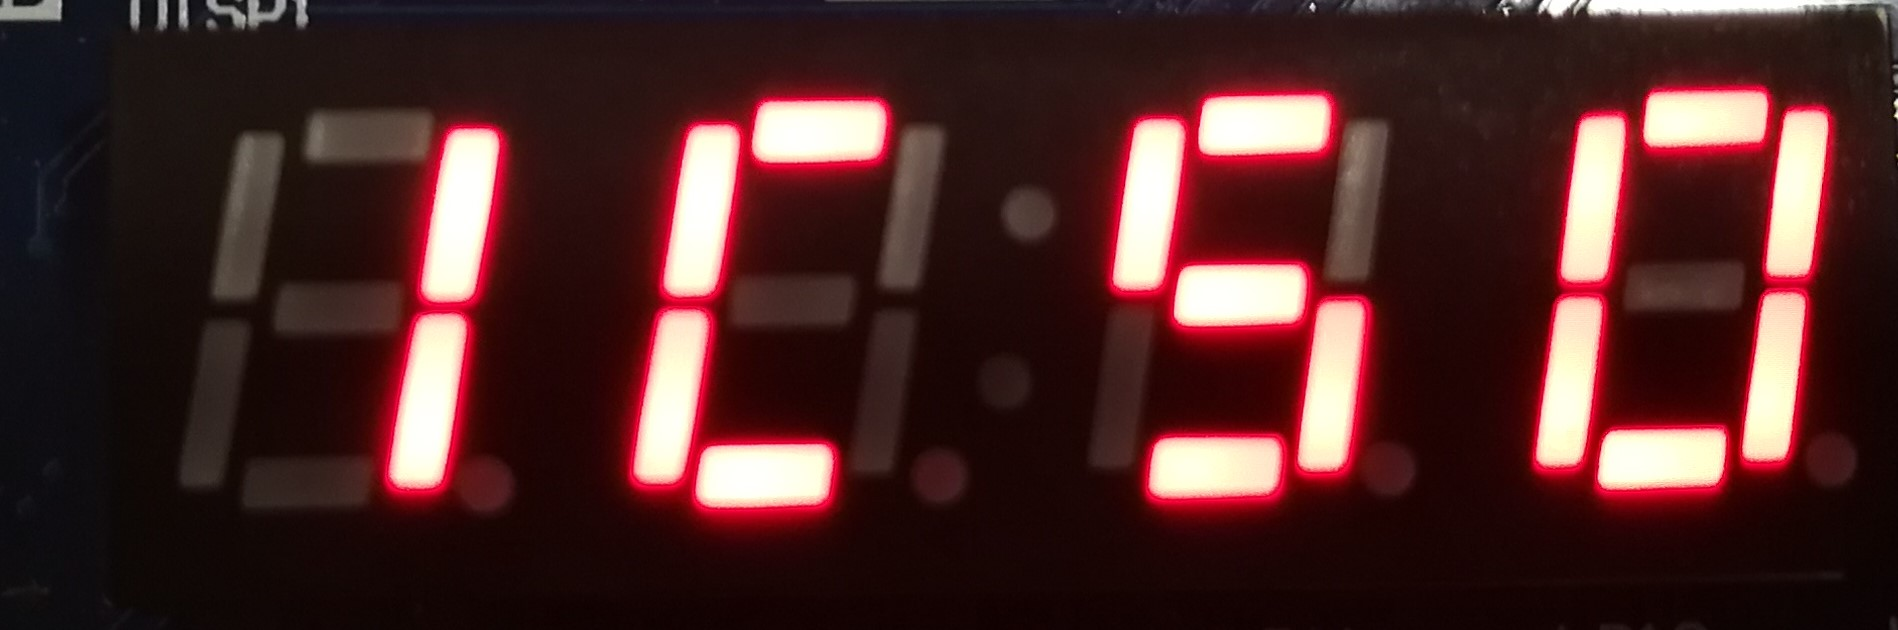
\includegraphics[width=0.3\linewidth]{fig/Implementation/0x1c_00.jpg}&
    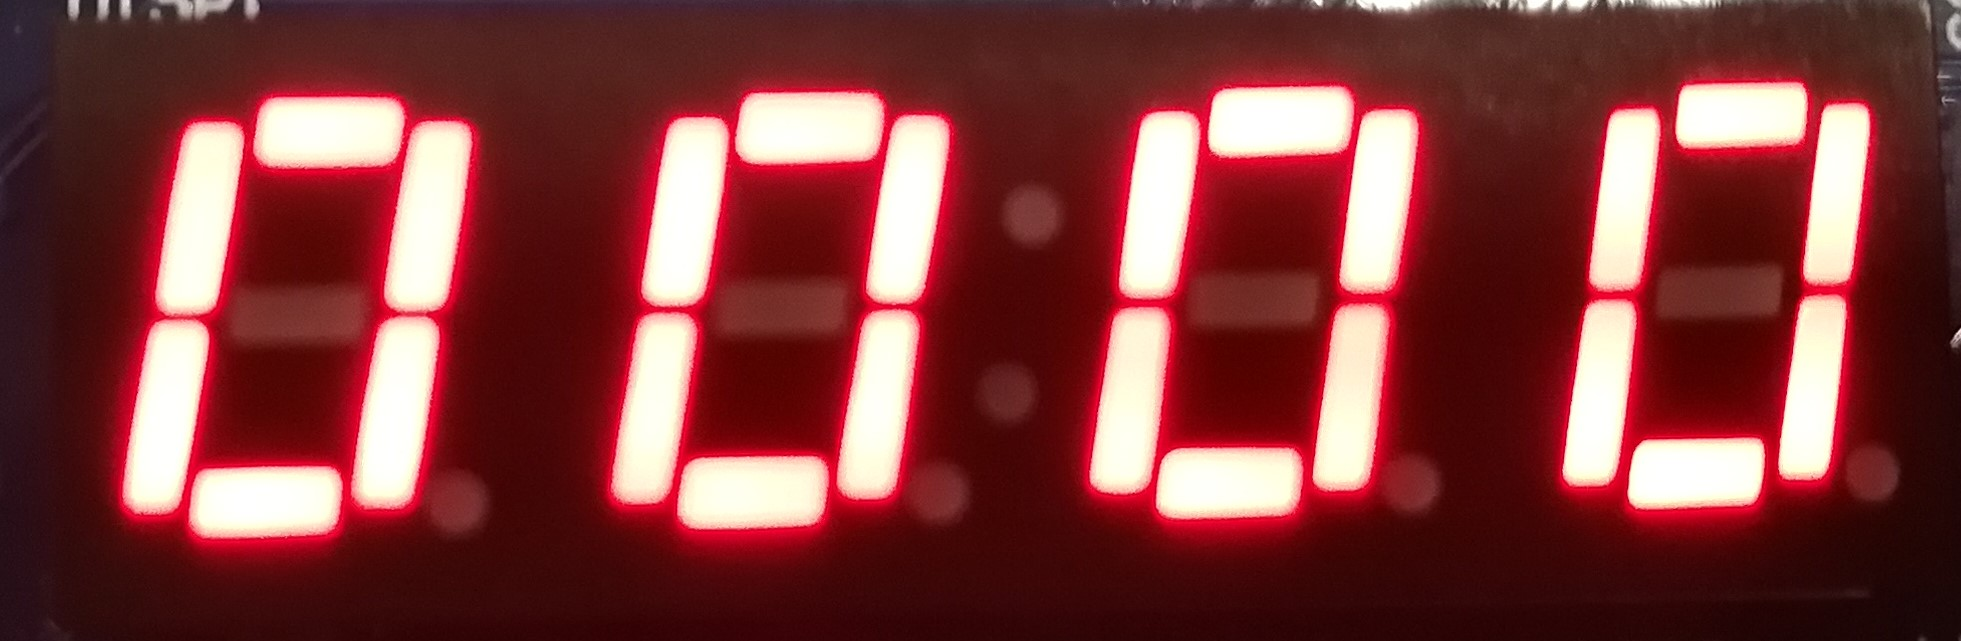
\includegraphics[width=0.3\linewidth]{fig/Implementation/0x1c_01.jpg}\\
    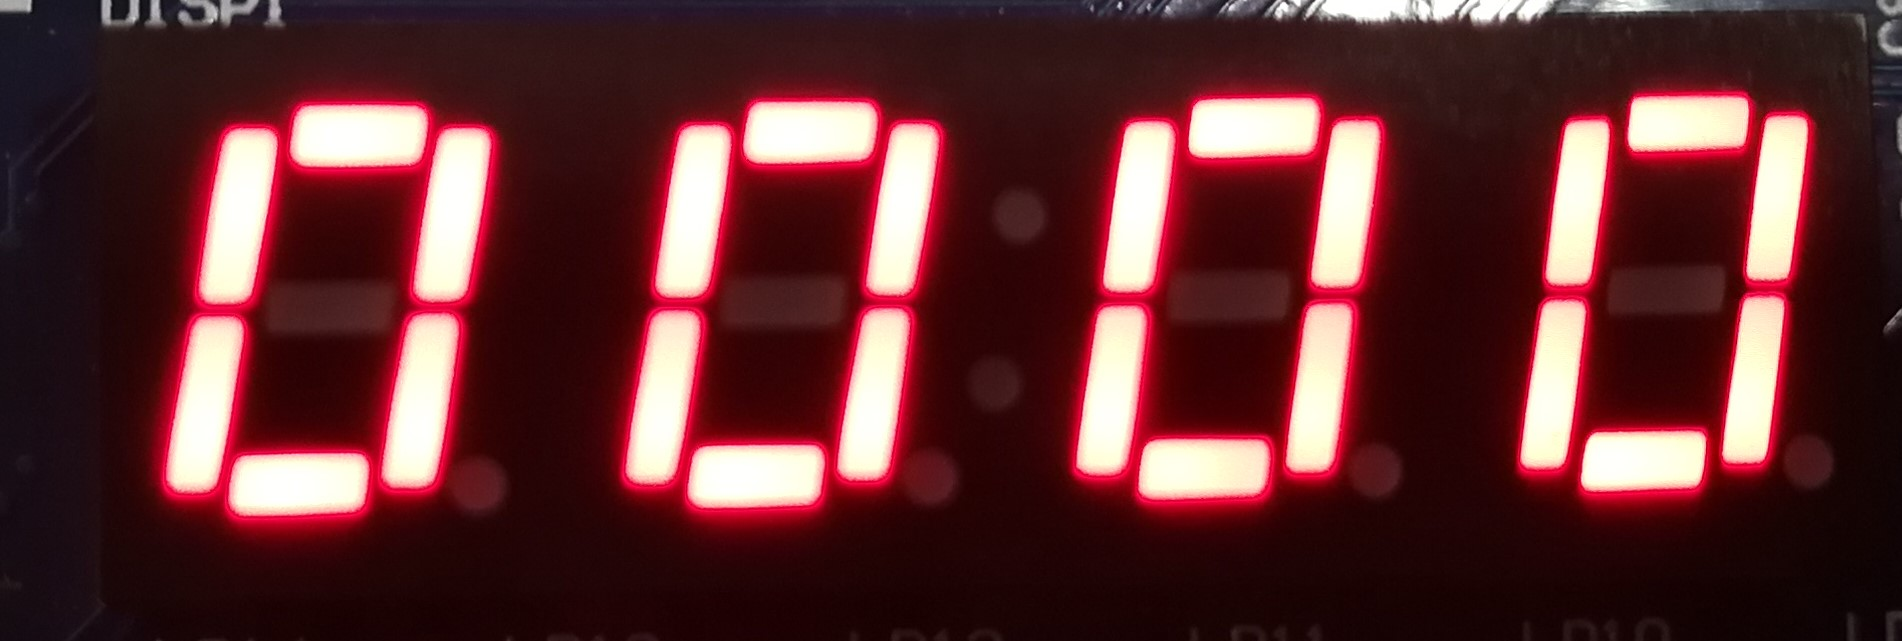
\includegraphics[width=0.3\linewidth]{fig/Implementation/0x1c_10.jpg}&
    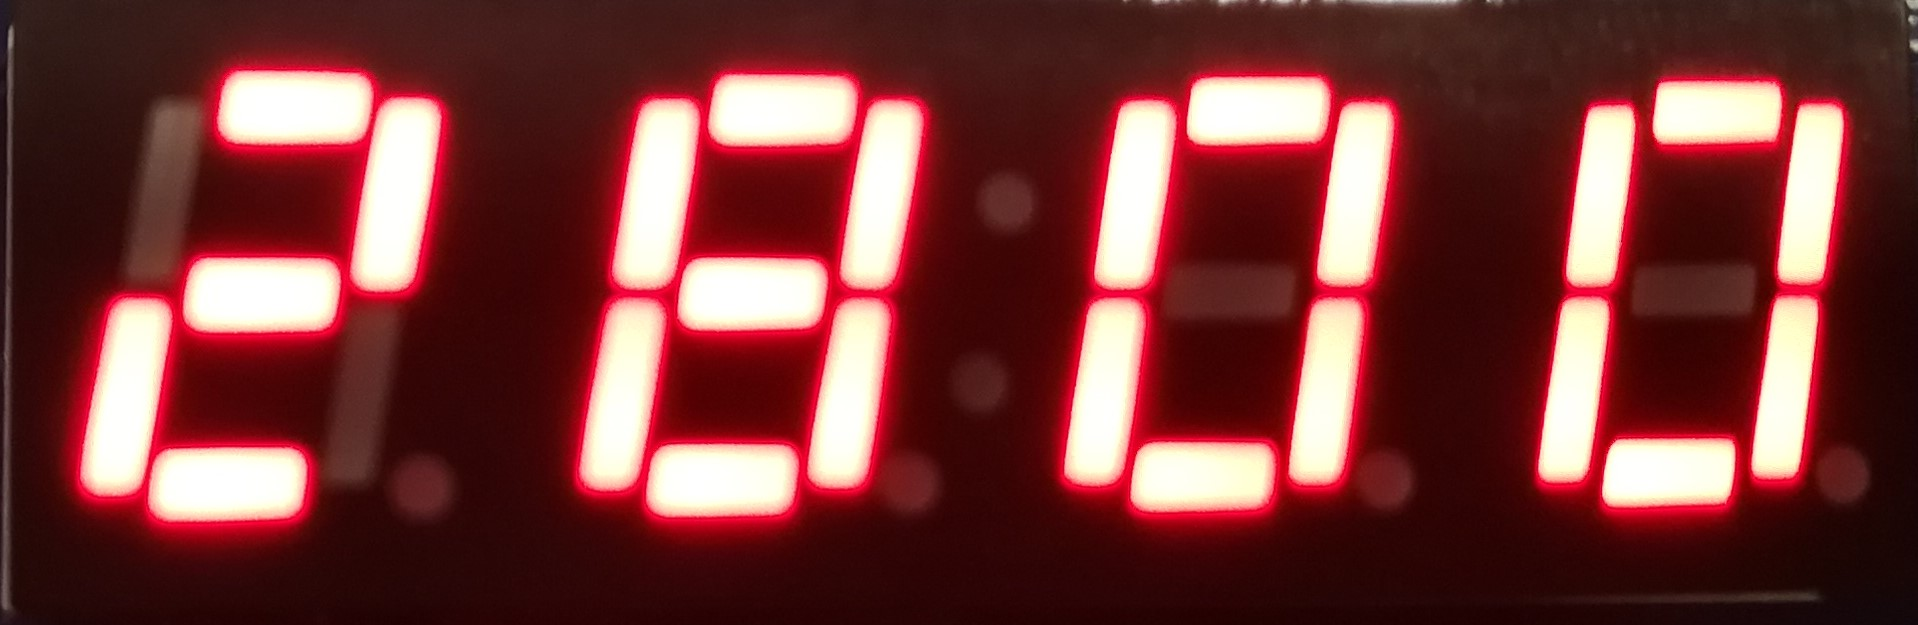
\includegraphics[width=0.3\linewidth]{fig/Implementation/0x1c_11.jpg}
    \end{tabular}
    \caption{0x1C结果}
    \end{figure}
    \item 0x54: \verb'lw $13, 4($1)'
    \begin{figure}[H]
    \centering
    \begin{tabular}{cc}
    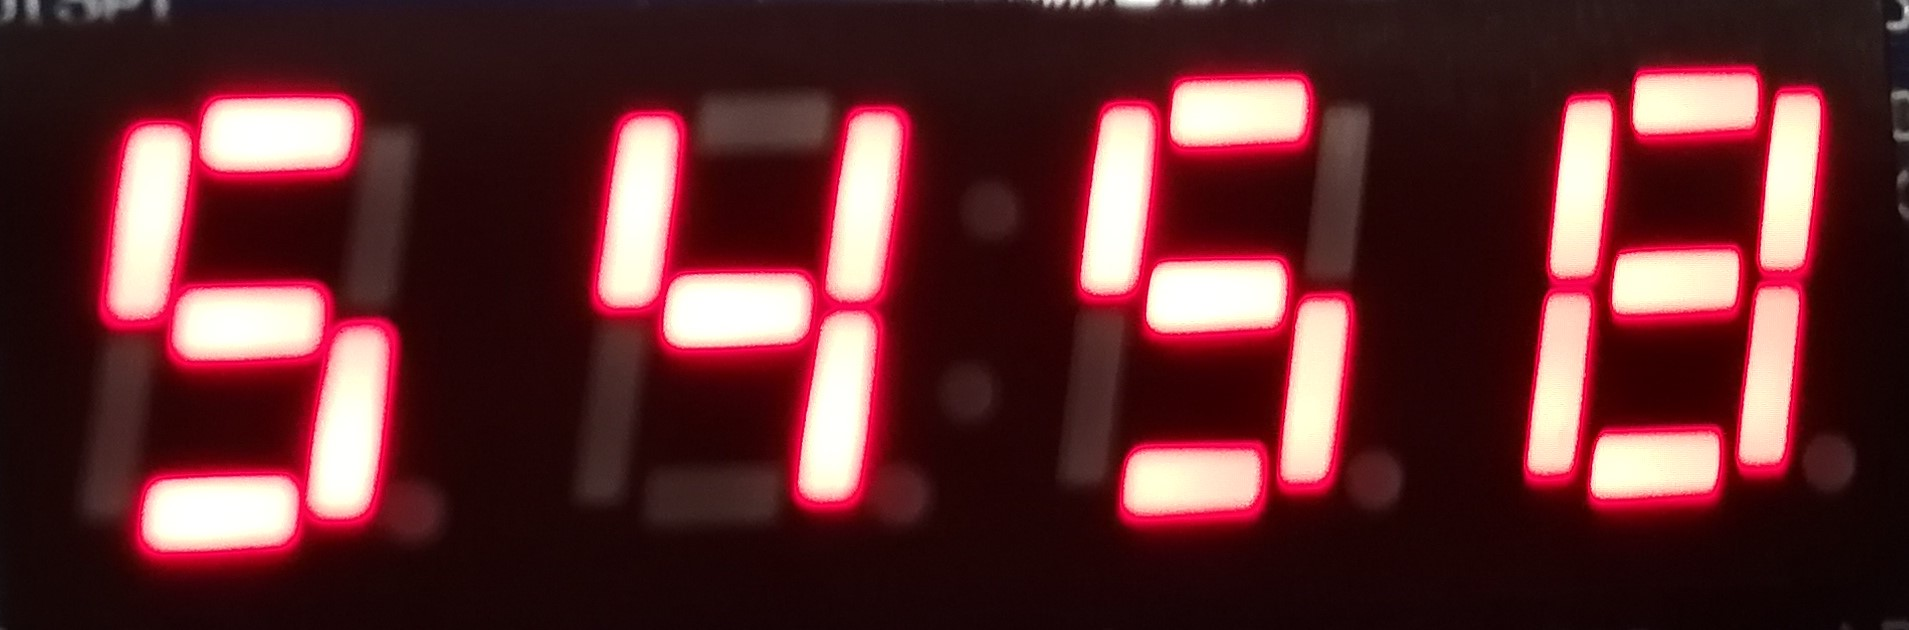
\includegraphics[width=0.3\linewidth]{fig/Implementation/0x54_00.jpg}&
    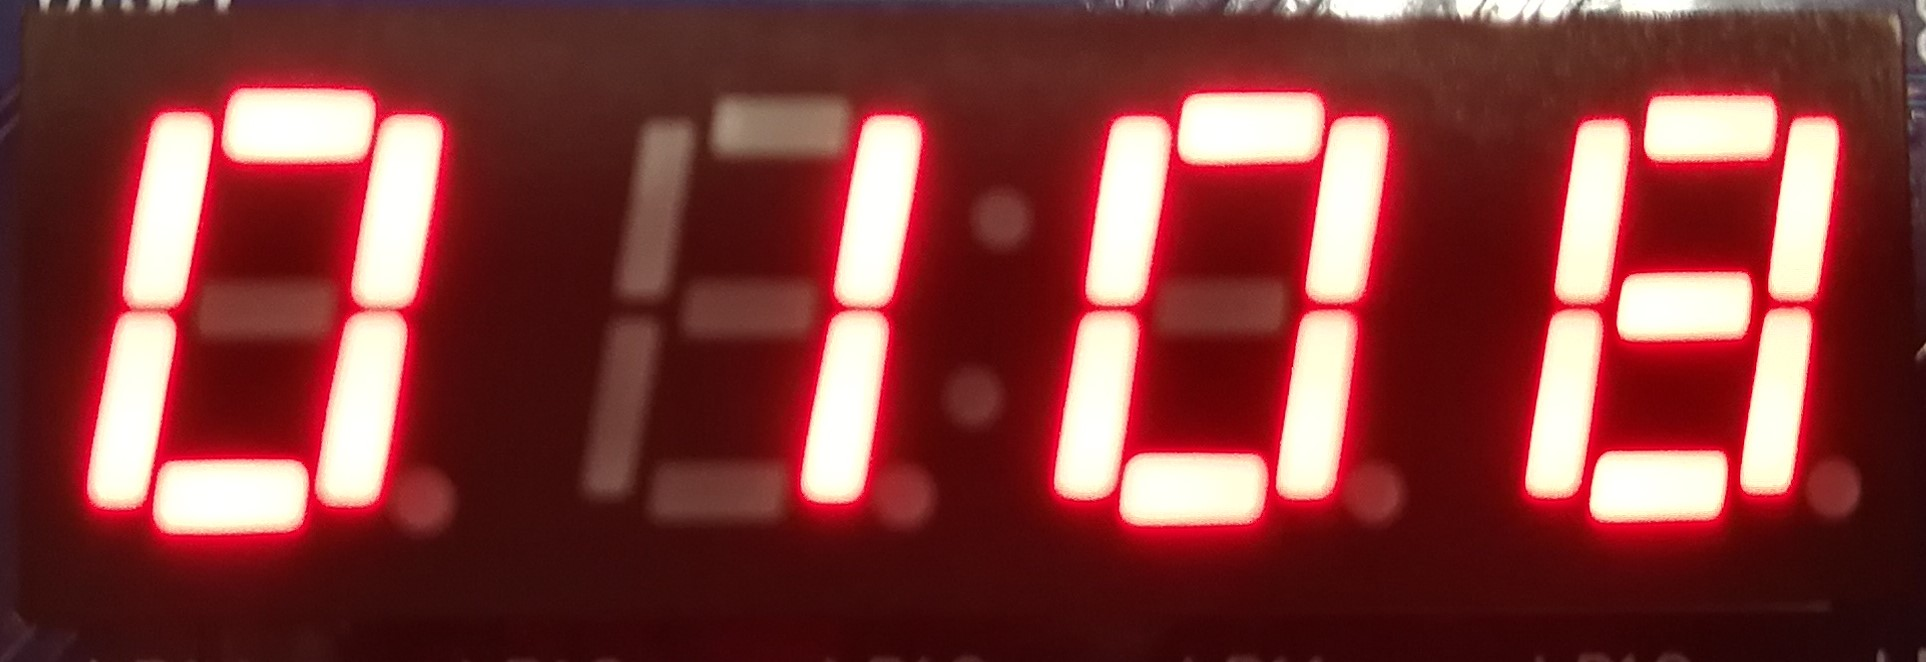
\includegraphics[width=0.3\linewidth]{fig/Implementation/0x54_01.jpg}\\
    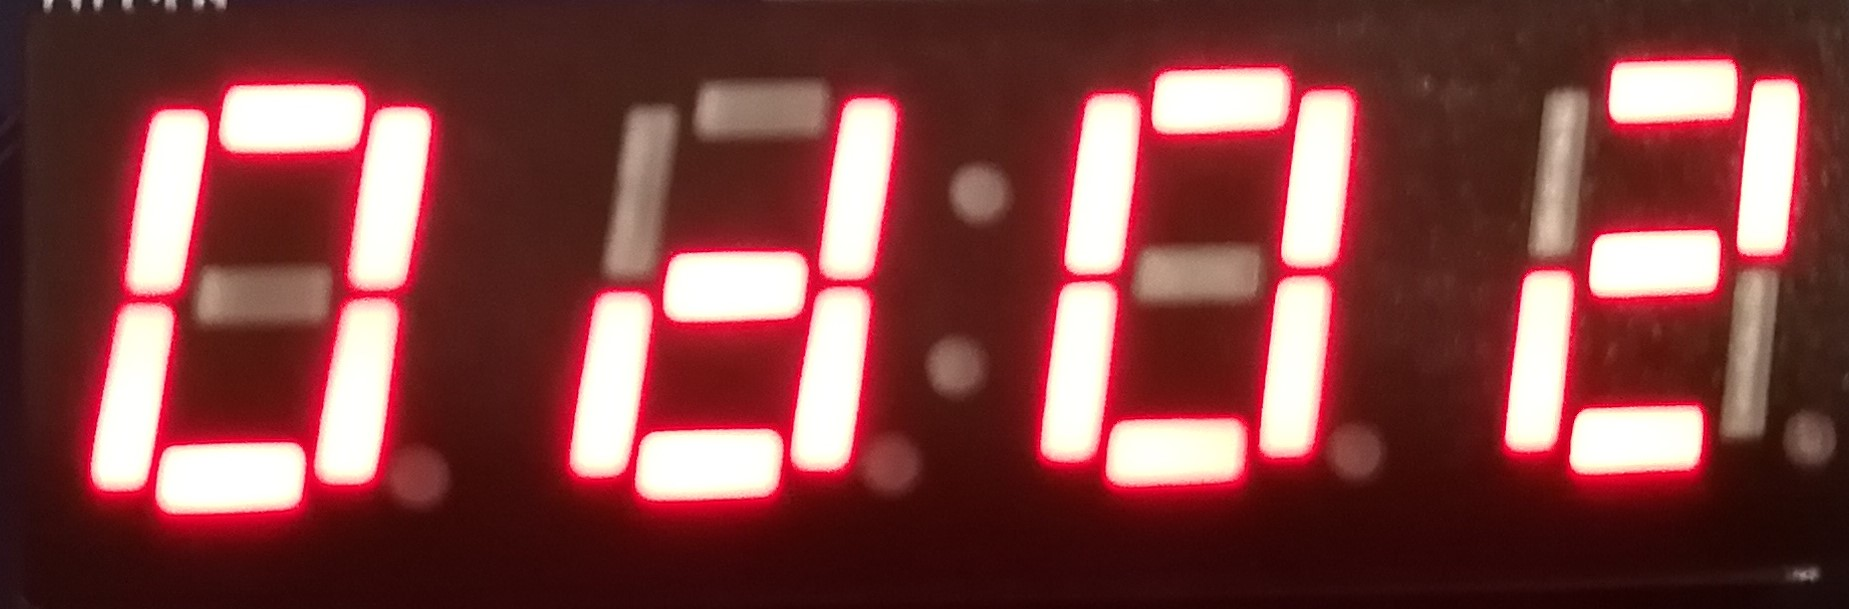
\includegraphics[width=0.3\linewidth]{fig/Implementation/0x54_10.jpg}&
    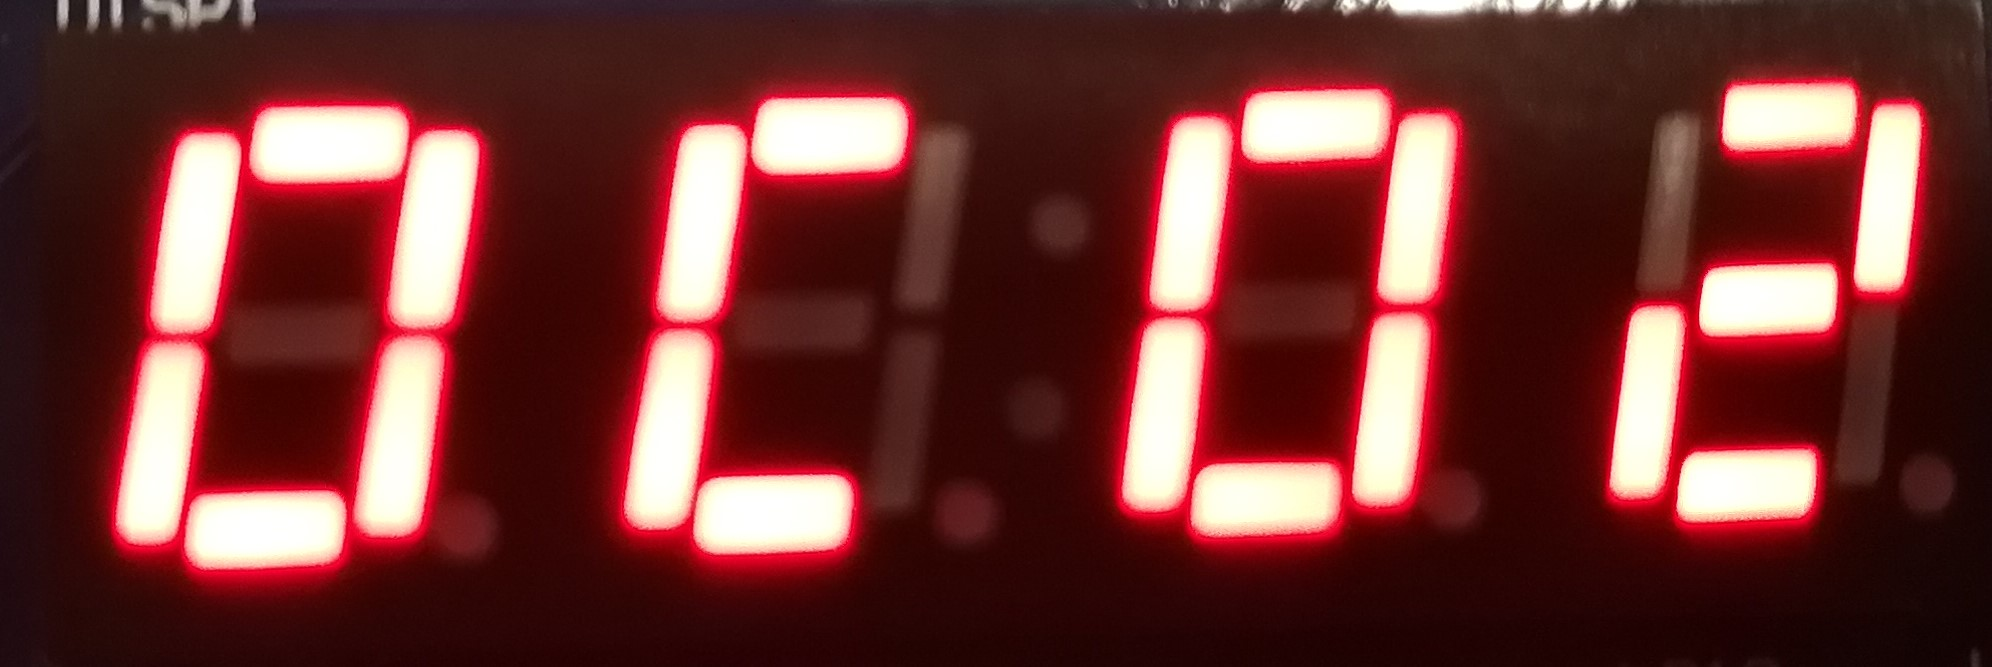
\includegraphics[width=0.3\linewidth]{fig/Implementation/0x54_11.jpg}
    \end{tabular}
    \caption{0x54结果}
    \end{figure}
    \item 0x58: \verb'jr $31'
    \begin{figure}[H]
    \centering
    \begin{tabular}{cc}
    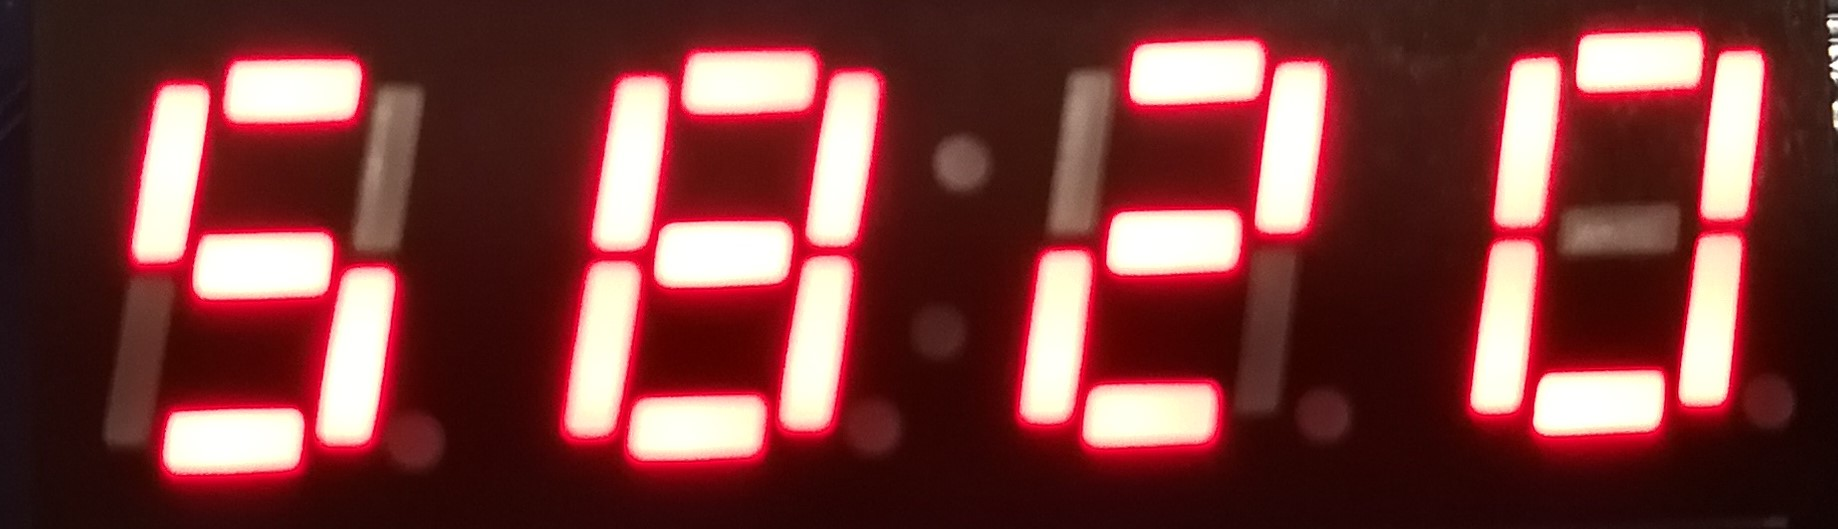
\includegraphics[width=0.3\linewidth]{fig/Implementation/0x58_00.jpg}&
    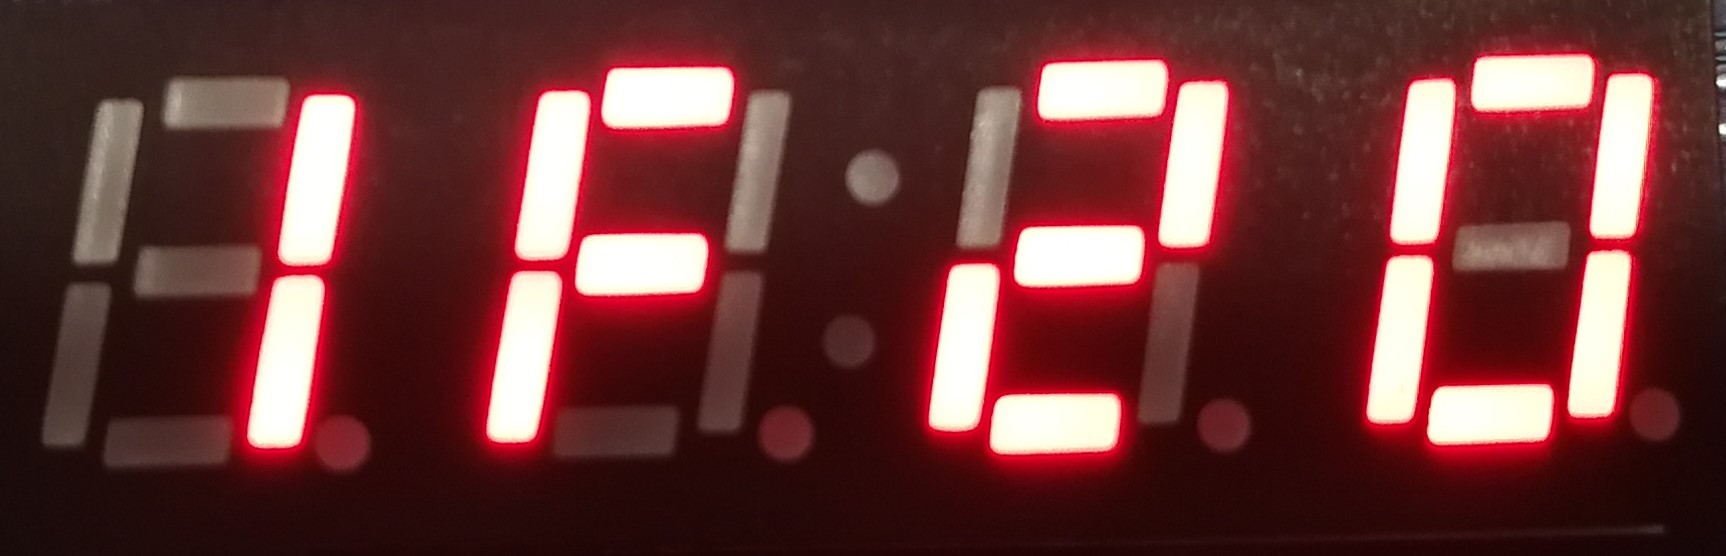
\includegraphics[width=0.3\linewidth]{fig/Implementation/0x58_01.jpg}\\
    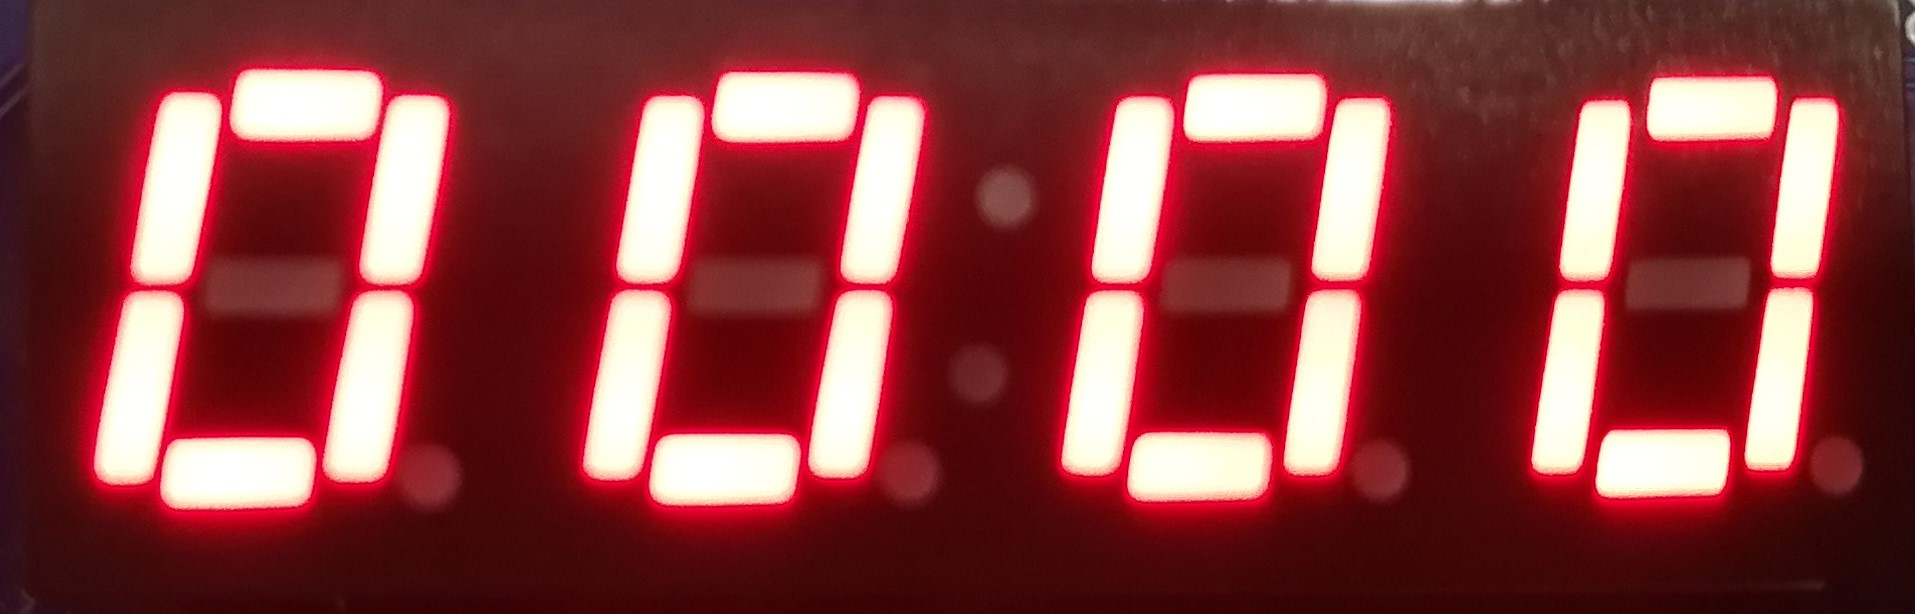
\includegraphics[width=0.3\linewidth]{fig/Implementation/0x58_10.jpg}&
    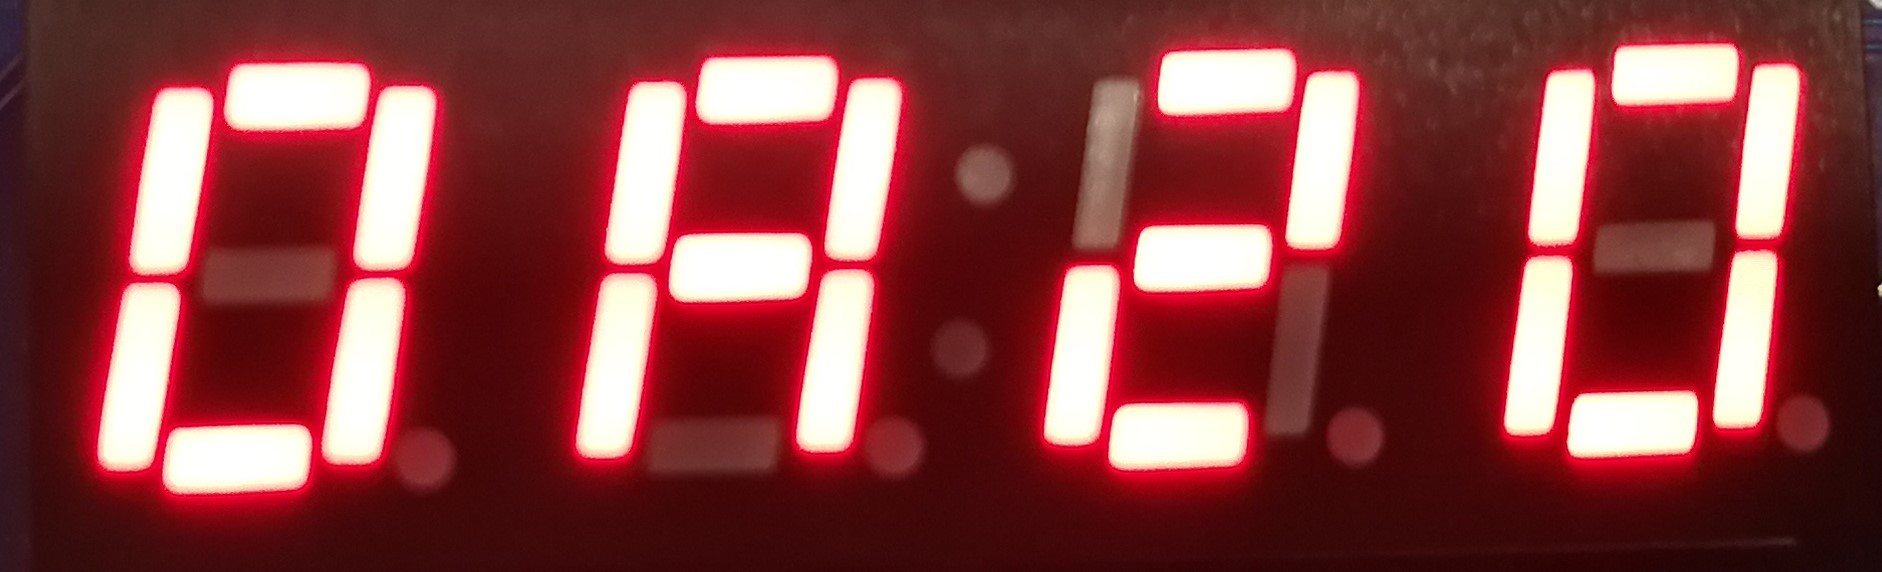
\includegraphics[width=0.3\linewidth]{fig/Implementation/0x58_11.jpg}
    \end{tabular}
    \caption{0x58结果}
    \end{figure}
\end{enumerate}

\section{实验心得}
% 体会和建议。(必须认真写,若过于简单,扣分!)
% (所写内容,如实验的整个过程中,所碰到的问题、所思考的问题等,以及最后如何获得解决,从中得到什么?等等,当然,还可能存在未解决的问题,或有所建议等。整个来说,就是总结一下本实验的情况,温故而知新,这个道理显而易见。)
\qquad 本次实验在单周期CPU的基础上继续搭建,重用了代码模块,只需分析清除控制信号和状态转移即可。虽然看似比较简单,具体实施时还是遇到了不少问题。
\par Verilog代码编写阶段:
\begin{enumerate}
    \item 当调整输入输出端口时,一定要记得将所有相关模块全部修改,如在控制单元中添加一个控制信号,则在CPU、CPU\_sim等模块中均需添加这个控制信号。
    \item 在模块输入参数最后常常多了一个逗号\verb',',会导致报错(\verb'ISE port connections mix')。
    \item 要判断好\verb'always @'内写的内容,是时序逻辑还是组合逻辑,不能混写,不能写多,也不能写少。
    \item 要在每个模块合适的位置对寄存器进行初始化\verb'initial',否则在仿真中会输出\verb'XXXX'。
    \item 多位的控制信号一定要记得写位宽[x:y],这个经常会漏,且不会报错
    \item 应在时钟下降沿才进行写入操作
\end{enumerate}
\par Vivado模拟仿真上板阶段:
\begin{enumerate}
    \item 延迟设置(如\verb'#10')具体上板实施时是会被忽略的
    \item 要做好门闩延迟(clock-to-Q)的设置,否则模块还没初始化完就开始操作,会出现很多问题,即对应的状态对应不上,会导致跳转指令无法正常跳转。
    \item 竞争与冒险的问题,在原来设计时,状态机只保存了当前状态。由于PC的更新和状态的更新是同步进行的,而由于具体电路不同路径延时不同的问题,导致PC更新时读取到的状态还是旧的,进而PC会被延迟到下一个周期才进行更新。全程的状态都会被延后一个周期,导致结果错误。因而这里很关键的一点在于状态机要设计成存储当前状态(currState)和下一状态(nextState),当下一状态为\verb'000'时就要考虑置PCWrite为1,并在当前状态为\verb'000'时对PC进行更新。这样既解决了设置延时的问题,又解决了竞争与冒险的问题。
\end{enumerate}
\par 总的来说,多周期CPU的设计实验让我更加熟悉了Verilog的语法,熟悉Vivado的使用,同时充分了解硬件设计与软件设计的巨大区别。硬件代码难以debug使得编写程序的效率极其低下,但这时一定不能心急,要冷静下来分析问题所在,并寻求方法解决它。同时,编写硬件程序时要拥有硬件思维,要考虑得更加周密,这些都是与编写软件程序很大的不同。


\section{期末总结}
\qquad 上了一整个学期的计算机组成原理的实验课,收获了比以往课程多更多的东西,也充分体会到了计算机硬件的乐趣与奥秘。总的来说,收获有以下几点:
\begin{enumerate}
    \item 明白指令集系统的原理,并学会用MIPS指令集编写简单的汇编程序
    \item 深刻了解CPU的工作原理,明白各指令的流向,理解并实现了各条数据通路
    \item 充分了解单周期CPU和多周期CPU的工作原理,并用Verilog具体实现了两种CPU,不仅进行了仿真,也进行了具体的上板实施
    \item 实现了简单的编译器,明白如何进行解析语义,完成汇编指令到机器二进制指令的转换
    \item 更加熟练Verilog代码的编写,掌握Vivado的使用,了解FPGA仿真综合跑实施的整个流程
    \item 学会通过观察波形在仿真阶段进行硬件程序的调试,学会通过观察数码管显示的内容在具体实施阶段进行硬件程序的调试
    \item 学会组织语言,涵盖所有要点,完成几十页的长实验报告
\end{enumerate}
\par 虽然这学期的计组实验课只让我们实现了三个项目(MIPS汇编语言程序设计、单周期CPU的设计与实现、多周期CPU的设计与实现),但是学到的东西真的非常多,下面结合我这三次项目的经历以及我个人学习计算机组成原理的感受,谈谈我自己的看法。
\par 首先,我充分感受到为什么我国至今没有开发芯片的核心技术,对于芯片设计仍处于起步阶段。这很大程度上是因为芯片设计的投入与回报的不对等性。硬件投入的人力财力都非常巨大,硬件程序不同于软件,开发周期时间长,debug的难度大。这学期的实验就充分体现了这几点。硬件开发要采用硬件思维,而不能用软件思维,要对问题充分考虑周全,要不然出现了bug会相当麻烦。尽管仿真没有出现问题,但是具体上板实施时却会出现各种各样的问题。这一方面是由于仿真工具无法全真模拟真实的硬件(特别是通路之间微小延时的差距),另一方面则是由于Vivado编译器对代码的检测非常不严格,对于可能出现的问题都选择忽略;更有甚者,连warning也不提醒,典型的例子即写少位宽的问题。尽管等号赋值右侧是3位的数据,但左侧没有声明[2:0],这种情况下vivado没有明显的报错,直接编译通过,给debug带来了极大的挑战。
\par 其次,我也了解到为什么MIPS指令集往往只用作学校的教学用,而很少有真实的硬件采用MIPS进行搭建,这很大一部分原因在于MIPS本身的局限性。对MIPS指令具体实现时会发现有些指令并不那么自然,要添加很多不必要的部件,设计一条新的数据通路。最明显的例子就是MIPS指令集中sll指令的实现,由于指令格式的不一致(5位的sa却存在最后的11位),CPU内就要添加多余的部件,并专门针对这一条指令进行数据通路的设计。这也在计算机发展了几十年以后,UCB仍要重新开发新的指令集RISC-V,并将其开源。就是因为传统的指令集肩负了太多历史包袱,越来越多新指令的出现,使得指令集变得十分笨重,也使得硬件的实施非常麻烦。
\par 第三点则从编程语言角度说的。单周期和多周期CPU的实现,我分别用Verilog各写了1000+行代码,然后就会发现Verilog的很多问题,比如它没有现代高级语言所拥有的很多设施,如递归的支持、面向对象(OOP)、高阶函数等等,换言之Verilog对于硬件操作的抽象做得比较弱,这直接导致了硬件工程师的开发效率极其低下。举个例子,由于没有参数化(parameterize)的设施,导致我在控制单元(Control Unit, CU)中添加一个新的信号,需要在CPU中的CU实例和输出端口添加该信号,还要在顶层模块的Show和CPU\_sim中添加输出端口,弄得十分麻烦。这还仅仅是两层封装,若遇到多层模块,稍微改动一下底层的模块,上层的建筑全部都得修改,可扩展性十分的差。同样因为这种低效率,UCB才开发了一门新的硬件语言Chisel(封装在Scala语言上),并已经在他们的EECS广泛使用。正是有这门相对高级的语言,才使得他们可以实现敏捷(Agile)开发,并成功制成了Rocket和BOOM等多款CPU核,还成功流片。这种前瞻性和实践性,是国内高校尚无法达到的。
\par 不仅仅是编程语言,编译器也是同样。由于手写RTL层级的硬件描述语言效率太低,所以才要有高层次综合(High Level Synthesis, HLS),直接将高级语言的程序直接编译为硬件描述语言的程序,但是限于现在的技术,HLS的编译效果不是特别好。至于下层的综合,尽管Vivado已经做了很大的努力去优化它,但其运行的时间依然非常长。像对我们这样一个简单实验中的CPU进行综合操作,一次都要花上$5\thicksim 10$分钟,这个开销是相当巨大的。这也反映了硬件开发反馈的效率极低,导致硬件难以设计难以debug、开发周期长。
\par 综上所述,硬件开发流程中依然有很多地方是做得不够完善的,还有极大的改进空间,值得我们继续去研究探索。最后真的非常感谢学院能够开设这门课,现在都倡导软硬件协同设计,不会硬件的计算机工程师就像是缺一条腿,只有清楚地知道CPU底层的硬件实现,才有可能写出更高质量的代码,共同促进软硬件的不断发展。

% !TEX root = main.tex

\newpage
\begin{multicols}{2}
\section{程序清单}
\label{sec:appendix}
\subsection{CPU主模块}
\begin{lstlisting}
timescale 1ns / 1ps

module CPU (
	input clk, reset,
	output RegDst,
	output ExtSel,
	output RegWrite, MemWrite,
	output ALUSrcA, ALUSrcB,
	output [2:0] ALUOp,
	output MemToReg,
	output Branch, Jump, Zero,
	output PCWrite,
	output [31:0] currPC, nextPC, instruction, alu_res,
	output wire [31:0] d1, d2, rsData, rtData,
	output wire [4:0] rs, rt, rd, sa, dbData
	);

	wire [5:0] opcode;
	wire [15:0] imm;
	wire [31:0] pc4;

	assign opcode = instruction[31:26];
	assign rs = instruction[25:21];
	assign rt = instruction[20:16];
	assign rd = instruction[15:11];
	assign sa = instruction[10:6];
	assign imm = instruction[15:0];

	PC pc(
		.clk(clk),
		.reset(reset),
		.PCWrite(PCWrite),
		.currPC(currPC),
		.nextPC(nextPC)
		);

	Adder add_pc4(
		.A(currPC),
		.B({{29{1'b0}},3'b100}),
		.res(pc4)
		);
	
	// instruction fetch (IF)
	InstructionMemory im(
		.address(currPC),
		.dataOut(instruction)
		);

	// instruction decode (ID)
	ControlUnit control(
		// input
		.opcode(opcode),
		.Zero(Zero),
		// output
		.RegDst(RegDst),
		.ExtSel(ExtSel),
		.RegWrite(RegWrite),
		.ALUSrcA(ALUSrcA),
		.ALUSrcB(ALUSrcB),
		.ALUOp(ALUOp),
		.MemToReg(MemToReg),
		.MemWrite(MemWrite),
		.Branch(Branch),
		.Jump(Jump),
		.PCWrite(PCWrite)
		);

	// execution (EXE)
	Registers reg_file(
		.clk(clk),
		.r1(rs),
		.r2(rt),
		.wr(mux_regdst.res),
		.RegWrite(RegWrite),
		.wd(mux_memToReg.res)
		// d1 -> mux_srcA.A
		// d2 -> mux_srcB.A / dm.dataIn
		);

	assign d1 = mux_srcA.res;
	assign d2 = mux_srcB.res;
	assign rsData = reg_file.d1;
	assign rtData = reg_file.d2;

	MUX5 mux_regdst(
		.Sel(RegDst),
		.A(rt),
		.B(rd)
		// res -> reg_file.wr
		);

	MUX mux_srcA(
		.Sel(ALUSrcA),
		.A(reg_file.d1),
		.B({{27{1'b0}},sa})
		// res -> alu.A
		);
	
	Extender extender(
		.Sel(ExtSel),
		.dataIn(imm)
		// dataOut -> mux_srcB.B / sl_16
		);

	MUX mux_srcB(
		.Sel(ALUSrcB),
		.A(reg_file.d2),
		.B(extender.dataOut)
		// res -> alu.B
		);

	ALU alu(
		.op(ALUOp),
		.A(mux_srcA.res),
		.B(mux_srcB.res),
		// res -> dm.address / mux_memToReg.A
		.res(alu_res),
		.zero(Zero)
		);

	// access memory (MEM)
	DataMemory dm(
		.clk(clk),
		.address(alu_res),
		.MemWrite(MemWrite),
		.dataIn(reg_file.d2)
		// dataOut -> mux_memToReg
		);

	// write back (WB)
	MUX mux_memToReg(
		.Sel(MemToReg),
		.A(alu_res),
		.B(dm.dataOut)
		// res -> reg_file.wd
		);

	assign dbData = mux_memToReg.res;

	// jump & branch
	ShiftLeft sl(
		.dataIn(extender.dataOut)
		// dataOut -> add_target.B
		);

	Adder add_target(
		.A(pc4),
		.B(sl.dataOut)
		// res -> mux_branch.B
		);

	MUX mux_branch(
		.Sel(Branch),
		.A(pc4),
		.B(add_target.res)
		// res -> mux_jump.A
		);

	MUX mux_jump(
		.Sel(Jump),
		.A(mux_branch.res),
		.B({pc4[31:28],instruction[25:0],2'b00}),
		.res(nextPC)
		);

endmodule
\end{lstlisting}

\subsection{指令存储器}
\begin{lstlisting}
module InstructionMemory (
	input [31:0] address,
	output [31:0] dataOut
	);
	
	reg [7:0] memory [0:255];

	// initialization
	initial $readmemb("D:/instruction.data",memory);
	// $display("Read in data successfully!");

	// output data (little endian)
	assign dataOut = {memory[address + 3],
					  memory[address + 2],
					  memory[address + 1],
					  memory[address]};

endmodule
\end{lstlisting}

\subsection{程序计数器(PC)}
\begin{lstlisting}
module PC (
    input clk,
    input reset,
    input PCWrite,
    input [31:0] nextPC,
    output reg [31:0] currPC
    );

    initial currPC = 0;

    always @(posedge clk or negedge reset) begin
        if (reset == 0)
            currPC <= 0;
        else if (PCWrite == 1)
            currPC <= nextPC;
    end

endmodule
\end{lstlisting}

\subsection{寄存器堆}
\begin{lstlisting}
module Registers (
    input clk,
    input [4:0] r1, // read reg #1 address
    input [4:0] r2, // read reg #2 address
    input [4:0] wr, // write reg address
    input RegWrite,
    input [31:0] wd, // write data
    output [31:0] d1, // read data 1
    output [31:0] d2 // read data 2
    );
    
    reg [31:0] register [0:31];
    
    // initialization
    integer i;
    initial begin
        for (i = 0; i < 32; i = i + 1)
            register[i] = 0;
    end

    // read data
    assign d1 = (r1 == 0) ? 0 : register[r1];
    assign d2 = (r2 == 0) ? 0 : register[r2];

    // write data
    always @(posedge clk) begin
        if (wr != 0 && RegWrite == 1)
            register[wr] <= wd;
    end

endmodule
\end{lstlisting}

\subsection{数据存储器}
\begin{lstlisting}
module DataMemory (
    input clk,
    input [31:0] address,
    input MemWrite,
    input [31:0] dataIn, // write data
    output [31:0] dataOut // read data
    );
    
    reg [7:0] memory [0:255];

    // initialization
    integer i;
    initial begin
        for (i = 0; i < 7; i = i + 1)
            memory[i] = 0;
    end

    // read data
    assign dataOut = {memory[address + 3], memory[address + 2], memory[address + 1], memory[address]};

    // write data
    always @(posedge clk) begin
        if (MemWrite == 1 && address >= 1 && address <= 255) begin
            // little endian
            memory[address + 3] <= dataIn[31:24];
            memory[address + 2] <= dataIn[23:16];
            memory[address + 1] <= dataIn[15:8];
            memory[address] <= dataIn[7:0];
        end
    end

endmodule
\end{lstlisting}

\subsection{控制单元}
\begin{lstlisting}
module ControlUnit (
    input [5:0] opcode,
    input Zero,
    output reg RegDst,
    output reg ExtSel,
    output reg RegWrite,
    output reg ALUSrcA,
    output reg ALUSrcB,
    output reg [2:0] ALUOp,
    output reg MemToReg,
    output reg MemWrite,
    output reg Branch,
    output reg Jump,
    output reg PCWrite
    );

    always @ (opcode or Zero) begin // Zero!
    	RegDst   <= 0;
		ExtSel   <= 0;
		RegWrite <= 1;
		ALUSrcA  <= 0;
		ALUSrcB  <= 0;
		ALUOp    <= 3'b000;
		MemToReg <= 0;
		MemWrite <= 0;
		Branch   <= 0;
		Jump     <= 0;
		PCWrite  <= 1;
    	case (opcode)
    		6'b000000: begin // add rd, rs, rt
    				RegDst <= 1;
    				end
    		6'b000001: begin // sub rd, rs, rt
    				RegDst <= 1;
    				ALUOp <= 3'b001;
    				end
    		6'b000010: begin // addiu rt, rs, imm
                    ExtSel <= 1; // ???
    				ALUSrcB <= 1;
    				end
    		6'b010000: begin // andi rt, rs, imm
    				ALUSrcB <= 1;
    				ALUOp <= 3'b100;
    				end
    		6'b010001: begin // and rd, rs, rt
    				RegDst <= 1;
    				ALUOp <= 3'b100;
    				end
    		6'b010010: begin // ori rt, rs, imm
    				ALUSrcB <= 1;
    				ALUOp <= 3'b011;
    				end
    		6'b010011: begin // or rd, rs, rt
    				RegDst <= 1;
    				ALUOp <= 3'b011;
    				end
    		6'b011000: begin // sll rd, rt, sa
    				RegDst <= 1;
    				ALUSrcA <= 1;
    				ALUOp <= 3'b010;
    				end
    		6'b011100: begin // slti rt, rs, imm
                    ExtSel <= 1;
                    ALUSrcB <= 1; // remember!
    				ALUOp <= 3'b110;
    				end
    		6'b100110: begin // sw rt, imm(rs)
    				ExtSel <= 1;
    				RegWrite <= 0;
    				ALUSrcB <= 1;
    				MemWrite <= 1;
    				end
    		6'b100111: begin // lw rt, imm(rs)
    				ExtSel <= 1;
    				ALUSrcB <= 1;
    				MemToReg <= 1;
    				end
    		6'b110000: begin // beq rs, rt, imm	
					ExtSel <= 1;
    				RegWrite <= 0;
    				ALUOp <= 3'b001;
    				Branch <= Zero;
					end
			6'b110001: begin // bne rs, rt, imm	
					ExtSel <= 1;
    				RegWrite <= 0;
    				ALUOp <= 3'b001;
    				Branch <= ~Zero; // (rs - rt == 0) ? 1 : 0 Not equal!
					end
			6'b110010: begin // bltz rs, imm
					ExtSel <= 1;
    				RegWrite <= 0;
    				ALUOp <= 3'b110; // compare sign
    				Branch <= ~Zero; // a < 0 ? 1 : 0
					end
			6'b111000: begin // j addr
    				RegWrite <= 0;
    				Jump <= 1;
					end
			6'b111111: begin // halt
					PCWrite <= 0;
					end
		endcase
	end
    
endmodule
\end{lstlisting}

\subsection{算术逻辑单元(ALU)}
\begin{lstlisting}
module ALU (
    input [2:0] op,
    input [31:0] A,
    input [31:0] B,
    output reg [31:0] res,
    output reg zero
    );
    
    initial begin
        res = 0;
    end
    
    always @(op or A or B) begin
        case (op)
            3'b000: res = A + B;
            3'b001: res = A - B;
            3'b010: res = B << A;
            3'b011: res = A | B;
            3'b100: res = A & B;
            3'b101: res = (A < B) ? 8'h00000001 : 0;
            3'b110: res = ((A < B && A[31] == B[31]) // both pos/neg num
                         || (A[31] == 1 && B[31] == 0)) // A neg B pos
                         ? 8'h00000001 : 0;
            3'b111: res = A ^ B;
        endcase
        zero <= (res == 0) ? 1 : 0;
    end

endmodule

module Adder (
    input [31:0] A,
    input [31:0] B,
    output [31:0] res
    );

    assign res = A + B;

endmodule

module ShiftLeft (
    input [31:0] dataIn,
    output [31:0] dataOut
    );
    
    assign dataOut = dataIn << 2;

endmodule
\end{lstlisting}

\subsection{多路选择器(MUX)}
\begin{lstlisting}
module MUX (
    input Sel,
    input [31:0] A,
    input [31:0] B,
    output reg [31:0] res
    );
    
    always @(Sel or A or B) begin
        res <= (Sel == 0) ? A : B;
    end

endmodule

module MUX5 (
    input Sel,
    input [4:0] A,
    input [4:0] B,
    output reg [4:0] res
    );
    
    always @(Sel or A or B) begin
        res <= (Sel == 0) ? A : B;
    end

endmodule
\end{lstlisting}

\subsection{数据扩展器}
\begin{lstlisting}
module Extender (
	input Sel,
	input [15:0] dataIn,
	output reg [31:0] dataOut
	);

	initial dataOut = 0;

	always @(Sel or dataIn) begin // dataIn!!!
		if (Sel == 0) // ZeroExt
			dataOut = {{16{1'b0}},dataIn[15:0]};
		else // SignExt
			dataOut = {{16{dataIn[15]}},dataIn[15:0]};
	end

endmodule
\end{lstlisting}

\subsection{仿真代码}
\begin{lstlisting}
module CPU_sim (
	output RegDst,
	output ExtSel,
	output RegWrite, MemWrite,
	output ALUSrcA, ALUSrcB,
	output [2:0] ALUOp,
	output MemToReg,
	output Branch, Jump, Zero,
	output PCWrite,
	output [31:0] currPC, nextPC, instruction, alu_res,
	output wire [31:0] d1, d2
	);
	
	reg clk;
	reg reset;

	CPU cpu(
		.clk(clk),
		.reset(reset),
		.RegDst(RegDst),
		.ExtSel(ExtSel),
		.RegWrite(RegWrite),
		.MemWrite(MemWrite),
		.ALUSrcA(ALUSrcA),
		.ALUSrcB(ALUSrcB),
		.ALUOp(ALUOp),
		.MemToReg(MemToReg),
		.Branch(Branch),
		.Jump(Jump),
		.Zero(Zero),
		.PCWrite(PCWrite),
		.currPC(currPC),
		.nextPC(nextPC),
		.instruction(instruction),
		.alu_res(alu_res),
		.d1(d1),
		.d2(d2)
		);

	initial begin
		clk = 1;
		reset = 0;
		// wait for initialization
		#80;
		reset = 1;
	end

	always #50 clk = ~clk;

endmodule
\end{lstlisting}

\subsection{分频计数器}
\begin{lstlisting}
module Counter(
    input clr, // clear, say reset
    input clk, // original clock
    output reg [1:0] count_4,
    output reg clk_seg
    );
    
    // display 10kHz
    reg [16:0] count_dis; // 26 bits to store count: 2^17 > 10^5
    always @ (posedge clk or posedge clr)
    begin
        if (clr == 1) // reset
        begin
            clk_seg <= 0;
            count_dis <= 0;
        end
        else if (count_dis == 50_000 - 1) // return 0
        begin
            clk_seg <= ~clk_seg;
            count_dis <= 0;
        end
        else
        begin
            clk_seg <= clk_seg;
            count_dis <= count_dis + 1;
        end
    end

    always @ (posedge clk_seg or posedge clr)
    begin
        if (clr == 1 || count_4 == 4)
            count_4 <= 0;
        else
            count_4 <= count_4 + 1;
    end

endmodule
\end{lstlisting}

\subsection{七段数码管}
\begin{lstlisting}
module SegDisplay (
	input [3:0] data,
	output reg [6:0] dispcode
	);

	always @(data)
		case(data)
			// 0: on    1: off
			1: dispcode = 7'b100_1111;
			2: dispcode = 7'b001_0010;
			3: dispcode = 7'b000_0110;
			4: dispcode = 7'b100_1100;
			5: dispcode = 7'b010_0100;
			6: dispcode = 7'b010_0000;
			7: dispcode = 7'b000_1111;
			8: dispcode = 7'b000_0000;
			9: dispcode = 7'b000_0100;
			10: dispcode = 7'b000_1000; // A
			11: dispcode = 7'b110_0000; // b
			12: dispcode = 7'b011_0001; // C
			13: dispcode = 7'b100_0010; // d
			14: dispcode = 7'b001_0000; // e
			15: dispcode = 7'b011_1000; // F
		endcase

endmodule
\end{lstlisting}

\subsection{写板电路}
\begin{lstlisting}
module Show(
	input clk,
	input clk_cpu,
	input reset,
	input [1:0] SW_in,
	output reg [6:0] dispcode,
	output reg [3:0] out
	);

	// synchronize
	reg in=1'b0;
	always @(posedge clk) begin
		in <= clk_cpu;
	end
	wire in_syn = in;

	// reduce jitter
	reg [15:0] inhistory = 16'h0000;
	reg in_detected = 1'b0;
	always @(posedge clk) begin
		inhistory <= { inhistory[14:0] , in_syn };
		if (inhistory == 16'b0011111111111111)
		  in_detected <= 1'b1;
		else
		  in_detected <= 1'b0;
	end

	wire seg_num; // not reg!

	Counter counter(
		.clk(clk),
		// output clock/counter
		.count_4(seg_num)
		);

	reg [31:0] firstNum;
	reg [31:0] secondNum;

	initial firstNum = 0;
	initial secondNum = 0;

	wire [31:0] currPC, nextPC, rsData, rtData, dbData, alu_res;
	wire [4:0] rs, rt;

	CPU cpu(
		// input
		.clk(in_detected),
		.reset(reset),
		// output
		.currPC(currPC),
		.nextPC(nextPC),
		.rs(rs),
		.rt(rt),
		.rsData(rsData),
		.rtData(rtData),
		.dbData(dbData),
		.alu_res(alu_res)
		);

	always @(SW_in) begin
		case (SW_in)
			2'b00: begin
				firstNum <= currPC;
				secondNum <= nextPC;
				end
			2'b01: begin
				firstNum <= {{27{1'b0}},rs};
				secondNum <= rsData;
				end
			2'b10: begin
				firstNum <= {{27{1'b0}},rt};
				secondNum <= rtData;
				end
			2'b11: begin
				firstNum <= alu_res;
				secondNum <= dbData;
				end
		endcase
	end

	SegDisplay seg1(
		.data(firstNum[7:4])
		// .dispcode
		);

	SegDisplay seg2(
		.data(firstNum[3:0])
		// .dispcode
		);

	SegDisplay seg3(
		.data(secondNum[7:4])
		// .dispcode
		);

	SegDisplay seg4(
		.data(secondNum[3:0])
		// .dispcode
		);

	always @ (seg_num or firstNum or secondNum)
		case (seg_num)
			0: begin
				out = 4'b1110;
				dispcode = seg4.dispcode;
				end
			1: begin
				out = 4'b1101;
				dispcode = seg3.dispcode;
				end
			2: begin
				out = 4'b1011;
				dispcode = seg2.dispcode;
				end
			3: begin
				out = 4'b0111;
				dispcode = seg1.dispcode;
				end
		endcase

endmodule
\end{lstlisting}

\subsection{限制文件(constraints.xdc)}
\begin{lstlisting}
set_property PACKAGE_PIN W5 [get_ports clk]
set_property PACKAGE_PIN T17 [get_ports clk_cpu]
set_property PACKAGE_PIN V17 [get_ports reset]
set_property PACKAGE_PIN R2 [get_ports {SW_in[1]}]
set_property PACKAGE_PIN T1 [get_ports {SW_in[0]}]
set_property PACKAGE_PIN W4 [get_ports {out[3]}]
set_property PACKAGE_PIN V4 [get_ports {out[2]}]
set_property PACKAGE_PIN U4 [get_ports {out[1]}]
set_property PACKAGE_PIN U2 [get_ports {out[0]}]
set_property PACKAGE_PIN W7 [get_ports {dispcode[6]}]
set_property PACKAGE_PIN W6 [get_ports {dispcode[5]}]
set_property PACKAGE_PIN U8 [get_ports {dispcode[4]}]
set_property PACKAGE_PIN V8 [get_ports {dispcode[3]}]
set_property PACKAGE_PIN U5 [get_ports {dispcode[2]}]
set_property PACKAGE_PIN V5 [get_ports {dispcode[1]}]
set_property PACKAGE_PIN U7 [get_ports {dispcode[0]}]

set_property IOSTANDARD LVCMOS33 [get_ports clk]
set_property IOSTANDARD LVCMOS33 [get_ports clk_cpu]
set_property IOSTANDARD LVCMOS33 [get_ports reset]
set_property IOSTANDARD LVCMOS33 [get_ports {SW_in[1]}]
set_property IOSTANDARD LVCMOS33 [get_ports {SW_in[0]}]
set_property IOSTANDARD LVCMOS33 [get_ports {out[3]}]
set_property IOSTANDARD LVCMOS33 [get_ports {out[2]}]
set_property IOSTANDARD LVCMOS33 [get_ports {out[1]}]
set_property IOSTANDARD LVCMOS33 [get_ports {out[0]}]
set_property IOSTANDARD LVCMOS33 [get_ports {dispcode[6]}]
set_property IOSTANDARD LVCMOS33 [get_ports {dispcode[5]}]
set_property IOSTANDARD LVCMOS33 [get_ports {dispcode[4]}]
set_property IOSTANDARD LVCMOS33 [get_ports {dispcode[3]}]
set_property IOSTANDARD LVCMOS33 [get_ports {dispcode[2]}]
set_property IOSTANDARD LVCMOS33 [get_ports {dispcode[1]}]
set_property IOSTANDARD LVCMOS33 [get_ports {dispcode[0]}]
\end{lstlisting}
\end{multicols}

\end{spacing}

\end{document}